\documentclass[15pt,a4paper]{article}
\usepackage[ ]{natbib} 
\usepackage[english]{babel}
\usepackage[utf8]{inputenc}
\usepackage[T1]{fontenc}
\usepackage{amsmath,amssymb,amsfonts,amsthm}
\usepackage[fleqn,tbtags]{mathtools}
\usepackage{dsfont} % Permet d'écrire la fonction indicatrice ds une formule math
\usepackage{authblk}
\usepackage{graphicx}
\usepackage{xcolor}
\usepackage{float}
\usepackage{geometry}
\geometry{margin = 1.2in}
\usepackage{booktabs}
\usepackage{multirow}
\usepackage{xr-hyper} % https://www.overleaf.com/learn/how-to/Cross_referencing_with_the_xr_package_in_Overleaf
\usepackage{hyperref}
%\usepackage{bbm}
\usepackage{array}
\usepackage[labelfont=bf]{caption}
\usepackage{subcaption}
\floatplacement{figure}{H}
\usepackage{floatpag} % Remove number when big plot or table
\floatpagestyle{empty} % Remove number when big plot or table
% \usepackage[mathlines]{lineno} % Continuous line numbering
% \linenumbers
\usepackage{setspace} % Set 1.5 line space
%\onehalfspacing % Set 1.5 line space
\doublespacing
\usepackage{mathpazo} 

\usepackage[normalem]{ulem} % Strikethough in LaTeX


%%% CODE TO PRESENT ALGORITHM IN THE TEXT
% \usepackage{algorithm}% http://ctan.org/pkg/algorithm
%\PassOptionsToPackage{noend}{algpseudocode}% comment out if want end's to show
% \usepackage{algpseudocode}% http://ctan.org/pkg/algorithmicx

\usepackage[ruled,vlined]{algorithm2e}

%\graphicspath{{image/}} % Fichier des images

\DeclareMathOperator{\Var}{\mathbb{V}\text{ar}}
\DeclareMathOperator{\Cov}{\mathbb{C}\text{ov}}
\DeclareMathOperator{\Corr}{\mathbb{C}\text{orr}}
\DeclareMathOperator{\Tra}{Trace}
\DeclareMathOperator{\Vect}{\mathbb{V}\text{ec}}
\DeclareMathOperator{\E}{\mathbb{E}}
\DeclareMathOperator*{\plim}{plim}
\DeclareMathOperator{\sign}{sign}
\DeclareMathOperator{\diag}{diag}
\newcommand*\mean[1]{\bar{#1}}
\newcommand{\norm}[1]{\left\lVert#1\right\rVert}
\newcommand{\argmin}{\operatornamewithlimits{argmin}}
\newcommand{\transpose}{{}^{\text{\sffamily T}}}
\newcommand{\bigO}{O}
\newcommand{\smallO}{o}
\DeclareMathOperator{\ERFE}{\textit{ERFE}}
\DeclareMathOperator{\QRFE}{\textit{QRFE}}
\DeclareMathOperator{\ER}{\textit{ER}}
\DeclareMathOperator{\QR}{\textit{QR}}
\DeclareMathOperator{\SE}{\textit{SE}}
\DeclareMathOperator{\SD}{\textit{SD}}
\DeclareMathOperator{\Reff}{\textit{Reff}}
\DeclareMathOperator{\FE}{\textit{FE}}

\DeclareMathOperator{\AR}{AR(1)} % Ar1
\DeclareMathOperator{\Exc}{Exc} 
\DeclareMathOperator{\Ind}{Ind}
\DeclareMathOperator{\QIC}{QIC}
\DeclareMathOperator{\asymQIC}{asymQIC}
\DeclareMathOperator{\CIC}{CIC}
\DeclareMathOperator{\asymCIC}{asymCIC}
\DeclareMathOperator{\GEEE}{GEEE}
\DeclareMathOperator{\GEE}{GEE}

%\newcommand\dsone{\mathbf{1}}

\newtheorem{theorem}{Theorem}%[section]
\newtheorem{lemma}{Lemma}%[theorem]
\newtheorem{proposition}{Proposition}%[theorem]
\newtheorem{corollary}{Corollary}%[theorem]

\renewcommand\qedsymbol{$\blacksquare$}

% Add some additional code to the preamble of File1.tex
\makeatletter
\newcommand*{\addFileDependency}[1]{% argument=file name and extension
  \typeout{(#1)}
  \@addtofilelist{#1}
  \IfFileExists{#1}{}{\typeout{No file #1.}}
}
\makeatother

\newcommand*{\myexternaldocument}[1]{%
    \externaldocument{#1}%
    \addFileDependency{#1.tex}%
    \addFileDependency{#1.aux}%
}


\setlength{\parindent}{0in} % Removing Paragraph Indenting in LaTeX
\setlength{\parskip}{1em}

\title{Weighted asymmetric least squares regression with fixed-effects} 



\myexternaldocument{0main}

% \author{}
\author[1,2]{Amadou Barry\footnote{Corresponding author: amadou.barry@mcgill.ca.} }
\author[3]{ Karim Oualkacha}
\author[3]{Arthur Charpentier}

\affil[1]{Departments of Epidemiology, Biostatistics and Occupational Health, McGill University, Montréal, Québec, Canada}
\affil[2]{Lady Davis Institute, Jewish General Hospital, Montréal, Québec, Canada}
\affil[3]{Department of Mathematics and Statistics, Université du Québec à Montréal, Montréal, Québec, Canada}
\date{\today}

\begin{document}
\maketitle

\section{Proof}

%%%888888888888888888888888888888888888888888888888888888888888888888888888888888888888888%%%888888888888888888888888888888888888888888888888888888888888888888888888888888888888888
\begin{proof}[\textbf{Proof of Theorem \ref{theo1_erfe}}]$ $ ~~\\~~\\
%%%888888888888888888888888888888888888888888888888888888888888888888888888888888888888888%%%888888888888888888888888888888888888888888888888888888888888888888888888888888888888888
The proof of \textbf{Theorem \ref{theo1_erfe}} is adapted from a proof of \citet{koenker_quantile_2004}. First, we present a philosophical approach and, secondly, a thorough one. We adopt a purely heuristic approach and ignore the complications introduced by the infinite dimensional nature of the incidental parameter. In the completed version, we explicitly concentrate out the incidental parameter before showing the asymptotic property of the parameter estimator of interest. The Lemma \ref{lem1_erfe} establishes the equivalence between the two approaches.
~~\\ 
~~\\
\textbf{Part 1.} Let $\mu_{ij\tau}= \boldsymbol{x}_{ij}\transpose\boldsymbol{\beta}_{\tau} + \boldsymbol{z}_{ij}\transpose\boldsymbol{\alpha}$ and consider the following objective function
\begin{equation} \label{risk_function_erfe}
    R_{nm}(\boldsymbol{\delta})=\sum_{i=1}^{n}\sum_{j=1}^{m}\rho_\tau \bigg\lbrace y_{ij}-\mu_{ij\tau}-\boldsymbol{z}_{ij}\transpose\boldsymbol{\delta}_0/\sqrt{m}-\boldsymbol{x}_{ij}
    \transpose\boldsymbol{\delta}_1/\sqrt{nm}\bigg\rbrace-\rho_\tau\lbrace y_{ij}-\mu_{ij\tau}\rbrace.
\end{equation}
The above objective function is a convex function of $\boldsymbol{\delta}$ that is minimized by 

%http://latex.wikia.com/wiki/Matrix_environments
\begin{equation}\label{delta_erfe}
\widehat{\boldsymbol{\delta}}=
\begin{pmatrix}
\widehat{\boldsymbol{\delta}}_0\\
\widehat{\boldsymbol{\delta}}_1\\
\end{pmatrix}
=
\begin{pmatrix}
\sqrt{m}(\widehat{\boldsymbol{\alpha}}-\boldsymbol{\alpha})\\
\sqrt{nm}(\widehat{\boldsymbol{\beta}}_{\tau}-\boldsymbol{\beta}_{\tau})\\
\end{pmatrix}.
\end{equation}
Our goal is to approximate $R_{nm}$ by a quadratic function with a unique minimizing value, and use results from \citet{hjort_asymptotics_2011} to show that $\widehat{\boldsymbol{\delta}}$ has the same asymptotic distribution of that minimizing value. This quadratic approximation is mainly composed by the Taylor expansion of the expected value and by a linear approximation function.
~~\\ 
~~\\
Let $\quad \widetilde{\boldsymbol{x}_{ij}}=(\boldsymbol{z}_{ij}\transpose,\boldsymbol{x}_{ij}\transpose)
\transpose, \qquad \widetilde{\boldsymbol{\delta}}=(\boldsymbol{\delta}_0\transpose/\sqrt{m},
\boldsymbol{\delta}_1\transpose/\sqrt{nm})\transpose\quad \mbox{ and } \quad \varepsilon_{ij\tau}=y_{ij}-\mu_{ij\tau}.$ The function $\E(\rho_\tau(\varepsilon_{ij\tau}-\widetilde{\boldsymbol{x}_{ij}}\transpose\widetilde{\boldsymbol{\delta}})-
\rho_\tau(\varepsilon_{ij\tau}))$ is convex, twice continuously differentiable and reaches its minimum at $\widetilde{\boldsymbol{\delta}}=\boldsymbol{0}.$ It can be represented in the neighbourhood of $\widetilde{\boldsymbol{\delta}}=\boldsymbol{0}$ as


\begin{equation}\label{Exploss1_erfe}
\begin{split}
    \E\big[\rho_\tau(\varepsilon_{ij\tau}-\widetilde{\boldsymbol{x}_{ij}}\transpose\widetilde{\boldsymbol{\delta}})-
    \rho_\tau(\varepsilon_{ij\tau})\big]&=\widetilde{\boldsymbol{\delta}}\transpose\widetilde{\boldsymbol{x}_{ij}}\E[\psi_\tau(\varepsilon_{ij\tau})]\widetilde{\boldsymbol{x}_{ij}}\transpose\widetilde{\boldsymbol{\delta}}  \\
    & -2\widetilde{\boldsymbol{\delta}}\transpose\widetilde{\boldsymbol{x}_{ij}}\E[\psi_\tau(\varepsilon_{ij\tau}).\varepsilon_{ij\tau}]   + \smallO{\norm{\widetilde{\boldsymbol{\delta}}}^2},
\end{split}
\end{equation}
where $\psi_\tau(\lambda)=\tau-\mathds{1}(\lambda<0).$ Since 


\begin{equation*}
   \argmin_{\boldsymbol{\delta}\;\in\;\mathbb{R}^{n+p}} \E\big[\rho_\tau(\varepsilon_{ij\tau}-\widetilde{\boldsymbol{x}_{ij}}\transpose\widetilde{\boldsymbol{\delta}})-\rho_\tau(\varepsilon_{ij\tau})\big]=\boldsymbol{0}
\end{equation*}
we have by the first order condition


\begin{equation}\label{FirstCondition_erfe}
    \E[\psi_\tau(\varepsilon_{ij\tau}).\varepsilon_{ij\tau}]=0,
\end{equation}
and equation (\ref{Exploss1_erfe}) can be reduced to:

\begin{equation}\label{Exploss2_erfe}
    \E\big[\rho_\tau(\varepsilon_{ij\tau}-\widetilde{\boldsymbol{x}_{ij}}\transpose\widetilde{\boldsymbol{\delta}})-
    \rho_\tau(\varepsilon_{ij\tau})
    \big]=\widetilde{\boldsymbol{\delta}}\transpose\widetilde{\boldsymbol{x}_{ij}}\E[\psi_\tau(\varepsilon_{ij\tau})]
    \widetilde{\boldsymbol{x}_{ij}}\transpose \widetilde{\boldsymbol{\delta}} + \smallO{\norm{\widetilde{\boldsymbol{\delta}}}^2}.
\end{equation}
The linear approximation function can be seen as a sort of Taylor expansion of $R_{nm}(\boldsymbol{\delta})$ around  $\boldsymbol{\delta}=0,$ see \citep{pollard_asymptotics_1991}. Define

\begin{equation}\label{Approx1_erfe}
D_{ij}(\varepsilon_{ij\tau})= -2\psi_\tau(\varepsilon_{ij\tau}).\varepsilon_{ij\tau}.
\end{equation}
Notice that by (\ref{FirstCondition_erfe}), \;$\E(D_{ij}(\varepsilon_{ij\tau}))=0.$ Define

\begin{equation*}
    r_{ij}(\widetilde{\boldsymbol{\delta}})=\rho_\tau(\varepsilon_{ij\tau}-\widetilde{\boldsymbol{x}_{ij}}\transpose
    \widetilde{\boldsymbol{\delta}})-\rho_\tau(\varepsilon_{ij\tau}) - \widetilde{\boldsymbol{\delta}}\transpose\widetilde{\boldsymbol{x}_{ij}} D_{ij}(\varepsilon_{ij\tau}).
\end{equation*}
Then
\begin{equation*}
\begin{split}
    R_{nm}(\widetilde{\boldsymbol{\delta}}) &=\sum_{i=1}^{n}\sum_{j=1}^{m}\bigg(\E\big[\rho_\tau(\varepsilon_{ij\tau}-
\widetilde{\boldsymbol{x}_{ij}}\transpose\widetilde{\boldsymbol{\delta}})-\rho_\tau(\varepsilon_{ij\tau})\big]\bigg) \\
    & + \sum_{i=1}^{n}\sum_{j=1}^{m}\widetilde{\boldsymbol{\delta}}\transpose\widetilde{\boldsymbol{x}_{ij}} D_{ij}(\varepsilon_{ij\tau}) + \sum_{i=1}^{n}\sum_{j=1}^{m} \bigg(r_{ij}(\widetilde{\boldsymbol{\delta}})-\E\big[r_{ij}(\widetilde{\boldsymbol{\delta}})\big]\bigg).
\end{split}
\end{equation*}
Using Lemma \ref{lemma1}, the objective function $R_{nm}(\widetilde{\boldsymbol{\delta}})$ reduce to 
\begin{equation}\label{risk_function1_erfe}
\begin{split}
    R_{nm}(\widetilde{\boldsymbol{\delta}}) &= \widetilde{\boldsymbol{\delta}}\transpose\sum_{i=1}^{n}\sum_{j=1}^{m}\bigg(\widetilde{\boldsymbol{x}_{ij}}
    \E[\psi_\tau(\varepsilon_{ij\tau})]\widetilde{\boldsymbol{x}_{ij}}\transpose\bigg)\widetilde{\boldsymbol{\delta}}+
    \widetilde{\boldsymbol{\delta}}\transpose\sum_{i=1}^{n}\sum_{j=1}^{m}
    \widetilde{\boldsymbol{x}_{ij}}D_{ij}(\varepsilon_{ij\tau}) + \bigO{\norm{\widetilde{\boldsymbol{\delta}}}^2} + \smallO{\norm{\widetilde{\boldsymbol{\delta}}}^2} \\
    &=    \widetilde{\boldsymbol{\delta}}\transpose\sum_{i=1}^{n}\sum_{j=1}^{m}\bigg(\widetilde{\boldsymbol{x}_{ij}}
    \E[\psi_\tau(\varepsilon_{ij\tau})]\widetilde{\boldsymbol{x}_{ij}}\transpose\bigg)\widetilde{\boldsymbol{\delta}}+
    \widetilde{\boldsymbol{\delta}}\transpose\sum_{i=1}^{n}\sum_{j=1}^{m}
    \widetilde{\boldsymbol{x}_{ij}}D_{ij}(\varepsilon_{ij\tau})
    + o_p(1)\\
    & \simeq \widetilde{\boldsymbol{\delta}}\transpose\sum_{i=1}^{n}\sum_{j=1}^{m}\bigg(\widetilde{\boldsymbol{x}_{ij}}
    \E[\psi_\tau(\varepsilon_{ij\tau})]\widetilde{\boldsymbol{x}_{ij}}\transpose\bigg)\widetilde{\boldsymbol{\delta}}+
    \widetilde{\boldsymbol{\delta}}\transpose\sum_{i=1}^{n}\sum_{j=1}^{m}
    \widetilde{\boldsymbol{x}_{ij}}D_{ij}(\varepsilon_{ij\tau}). \\
\end{split}
\end{equation}
By replacing $\; \widetilde{\boldsymbol{x}_{ij}}=(\boldsymbol{z}_{ij}\transpose,\boldsymbol{x}_{ij}\transpose)\transpose \; \mbox{ and } \; \widetilde{\boldsymbol{\delta}}=(\boldsymbol{\delta}_0\transpose/\sqrt{m},
\boldsymbol{\delta}_1\transpose/\sqrt{nm})\transpose$ by their initial value, we have
\begin{align*}
\begin{split}
   {}& R_{nm}(\boldsymbol{\delta}) = \\
    & -2\frac{1}{\sqrt{m}}\sum_{i=1}^{n}\sum_{j=1}^{m}(\boldsymbol{z}_{ij}\transpose\boldsymbol{\delta}_0 + \boldsymbol{x}_{ij}\transpose\boldsymbol{\delta}_1/\sqrt{n})
     \psi_\tau(y_{ij}-\mu_{ij\tau}).(y_{ij}-\mu_{ij\tau})\\ 
    & +\frac{1}{m}\sum_{i=1}^{n}\sum_{j=1}^{m}\E[\psi_\tau(y_{ij}-\mu_{ij\tau})](\boldsymbol{z}_{ij}\transpose\boldsymbol{\delta}_0+\boldsymbol{x}_{ij} \transpose\boldsymbol{\delta}_1/\sqrt{n})^2
\end{split}\\
\begin{split}
    {}&= -2\frac{1}{\sqrt{m}}\bigg[\boldsymbol{\delta}_0\transpose\boldsymbol{Z}\transpose\boldsymbol{\Psi}_\tau(\boldsymbol{\varepsilon}_{\tau})\boldsymbol{\varepsilon}_{\tau} +\boldsymbol{\delta}_1\transpose/\sqrt{n}\boldsymbol{X}\transpose\boldsymbol{\Psi}_\tau(\boldsymbol{\varepsilon}_{\tau})\boldsymbol{\varepsilon}_{\tau}\bigg]\\
    & + \frac{1}{m}\bigg[ \boldsymbol{\delta}_0\transpose\boldsymbol{Z}\transpose\E[\boldsymbol{\Psi}_\tau(\boldsymbol{\varepsilon}_{\tau})]\boldsymbol{Z}
    \boldsymbol{\delta}_0 + 2\boldsymbol{\delta}_0\transpose\boldsymbol{Z}\transpose\E[\boldsymbol{\Psi}_\tau(\boldsymbol{\varepsilon}_{\tau})]
    \boldsymbol{X}\boldsymbol{\delta}_1/\sqrt{n} +\boldsymbol{\delta}_1\transpose\boldsymbol{X}\transpose\E[\boldsymbol{\Psi}_\tau(\boldsymbol{\varepsilon}_{\tau})]\boldsymbol{X}
    \boldsymbol{\delta}_1/n\bigg]\\
    & = R_{nm}^{(1)}(\boldsymbol{\delta}) + R_{nm}^{(2)}(\boldsymbol{\delta})
\end{split}\\
\end{align*}
~~\\
The condition \textbf{A2} and \textbf{A3} imply a Lindberg condition and we have
\begin{equation*}
    R_{nm}^{(1)}(\boldsymbol{\delta})=-2\frac{1}{\sqrt{m}}\Big[\boldsymbol{\delta}_0\transpose\boldsymbol{Z}
    \transpose+\boldsymbol{\delta}_1\transpose/\sqrt{n}\boldsymbol{X}\transpose\Big]\boldsymbol{\Psi}_\tau(\boldsymbol{\varepsilon}_{\tau})\boldsymbol{\varepsilon}_{\tau}
    \xrightarrow{d}-2\boldsymbol{\delta}\transpose\boldsymbol{B}.
\end{equation*}
While by condition \textbf{A2}


\begin{equation*}
\begin{split}
    R_{nm}^{(2)}(\boldsymbol{\delta}) 
    & =  \frac{1}{m}\bigg[ \boldsymbol{\delta}_0\transpose\boldsymbol{Z}\transpose\E[\boldsymbol{\Psi}_\tau(\boldsymbol{\varepsilon}_{\tau})]\boldsymbol{Z}
    \boldsymbol{\delta}_0 + 2\boldsymbol{\delta}_0\transpose\boldsymbol{Z}\transpose\E[\boldsymbol{\Psi}_\tau(\boldsymbol{\varepsilon}_{\tau})]
    \boldsymbol{X}\boldsymbol{\delta}_1/\sqrt{n} +\boldsymbol{\delta}_1\transpose\boldsymbol{X}\transpose\E[\boldsymbol{\Psi}_\tau(\boldsymbol{\varepsilon}_{\tau})]\boldsymbol{X}
    \boldsymbol{\delta}_1/n\bigg]\\
    & \rightarrow \boldsymbol{\delta}\transpose \boldsymbol{D}_1 \boldsymbol{\delta}.
\end{split}
\end{equation*}
Thus the limiting form of the objective function is
\begin{equation*}
    R_0(\boldsymbol{\delta})=-2\boldsymbol{\delta}\transpose\boldsymbol{B}+\boldsymbol{\delta}\transpose \boldsymbol{D}_1 \boldsymbol{\delta}
\end{equation*}
where $\boldsymbol{B}$ is a zero mean Gaussian vector with covariance matrix $\boldsymbol{D}_0.$ The objective function $R_{nm}$ is convex and its limiting form $R_0$ has a unique minimum. Therefore, by \textbf{Theorem}\ref{hjort2}, $\widehat{\boldsymbol{\delta}}$ converge to the argmin of $R_0.$
~~\\
~~\\
\textbf{Part 2.} In the precedent proof we overlook the complications related to the infinite dimensional nature of $\boldsymbol{\alpha}.$ \citet{koenker_quantile_2004}, following \citep{Bickel1975,ruppert_trimmed_1980}, used the Bahadur-Kiefer representation of the incidental parameter in order to concentrate out its effect and express the objective function solely in terms of the finite dimensional parameter $\boldsymbol{\beta}.$ With the smoothness of the asymmetric least square loss, we can use the first order condition to represent the incidental parameter as a function of the structural parameter. 
\newline
\newline
Consider the following objective function
\begin{equation*}
\begin{split}
   R_{nm}(\boldsymbol{\delta})&= 
   -2\frac{1}{\sqrt{m}}\sum_{i=1}^{n}\sum_{j=1}^{m}(\boldsymbol{z}_{ij}\transpose\boldsymbol{\delta}_0
        + \boldsymbol{x}_{ij}\transpose\boldsymbol{\delta}_1/\sqrt{n})\psi_\tau(y_{ij}-\mu_{ij\tau}).
        (y_{ij}-\mu_{ij\tau})\\
        & +\frac{1}{m}\sum_{i=1}^{n}\sum_{j=1}^{m}\E[\psi_\tau(y_{ij}-\mu_{ij\tau})]
   (\boldsymbol{z}_{ij}\transpose\boldsymbol{\delta}_0+\boldsymbol{x}_{ij} \transpose\boldsymbol{\delta}_1/\sqrt{n})^2.
\end{split}
\end{equation*}
This function is twice derivable and the first order condition gives us the exact representation of the incidental parameter
\begin{equation*}
   \frac{\widehat{\delta}_{0i}}{\sqrt{m}}=\frac{1}{m\overline{\boldsymbol{\psi}}_i}\sum_{k=1}^{m}\psi_{\tau}(y_{ik}-\mu_{ik\tau})(y_{ik}-\mu_{ik\tau})-\frac{1}{m\overline{\boldsymbol{\psi}}_i}
    \sum_{k=1}^{m}\E\big[\psi_{\tau}(y_{ik}-\mu_{ik\tau})\big]\boldsymbol{x}_{ik}\transpose\frac{\boldsymbol{\delta}_1}{\sqrt{nm}},
\end{equation*}
where $\overline{\boldsymbol{\psi}}_i=m^{-1}\sum_{k=1}^{m} \E\Big[\psi_{\tau}\big(y_{ik}-\mu_{ik\tau}\big)\Big].$
Substituting $\frac{\widehat{\delta}_{0i}}{\sqrt{m}}$ we have
\begin{equation*}
\begin{split}
   {}&\frac{\widehat{\boldsymbol{\delta}}_{1}}{\sqrt{mn}}=\bigg(\sum_{i=1}^{n}\sum_{j=1}^{m}\boldsymbol{x}_{ij}\E[\psi_\tau(y_{ij}-\mu_{ij\tau})]\Big[\boldsymbol{x}_{ij}\transpose-\frac{1}{m
   \overline{\boldsymbol{\psi}}_i}
   \sum_{k=1}^{m}\E\big[\psi_{\tau}(y_{ik}-\mu_{ik\tau})\big]\boldsymbol{x}_{ik}\transpose\Big]\bigg)^{-1}\\
   {}&\times \bigg(\sum_{i=1}^{n}\sum_{j=1}^{m}\boldsymbol{x}_{ij}\psi_\tau(y_{ij}-\mu_{ij\tau})
   (y_{ij}-\mu_{ij\tau})\\
   {}& -\sum_{i=1}^{n}\sum_{j=1}^{m}\boldsymbol{x}_{ij}\E[\psi_\tau(y_{ij}-
   \mu_{ij\tau})]\Big[\frac{1}{m\overline{\boldsymbol{\psi}}_i}\sum_{k=1}^{m}
   \psi_{\tau}(y_{ik}-\mu_{ik})(y_{ik}-\mu_{ik})\Big]\bigg).
\end{split}
\end{equation*}
Note that,
\begin{equation*}
\begin{split}
   {}& \sum_{i=1}^{n}\sum_{j=1}^{m}\boldsymbol{x}_{ij}\E[\psi_\tau(y_{ij}-\mu_{ij\tau})]\Big[\boldsymbol{x}_{ij}\transpose-\frac{1}{m\overline{\boldsymbol{\psi}}_i}  \sum_{k=1}^{m}\E\big[\psi_{\tau}(y_{ik}-\mu_{ik})\big]\boldsymbol{x}_{ik}\transpose\Big]\\
   {}&=\boldsymbol{X}\transpose\E[\boldsymbol{\Psi}_\tau(\boldsymbol{\varepsilon}_{\tau})]\boldsymbol{X}-\boldsymbol{X}\transpose\boldsymbol{P}_{\boldsymbol{Z}}\transpose\E[\boldsymbol{\Psi}_\tau(\boldsymbol{\varepsilon}_{\tau})]\boldsymbol{X}\\
   {}&=\boldsymbol{X}\transpose[\mathbb{I}-\boldsymbol{P}_{\boldsymbol{Z}}]\E[\boldsymbol{\Psi}_\tau(\boldsymbol{\varepsilon}_{\tau})]\boldsymbol{X}\\   
   {}&=\boldsymbol{X}\transpose\boldsymbol{M}_{\boldsymbol{Z}}\transpose\E[\boldsymbol{\Psi}_\tau(\boldsymbol{\varepsilon}_{\tau})]\boldsymbol{X}\\
   {}&=\boldsymbol{X}\transpose\boldsymbol{M}_{\boldsymbol{Z}}\transpose\boldsymbol{M}_{\boldsymbol{Z}}\transpose\E[\boldsymbol{\Psi}_\tau(\boldsymbol{\varepsilon}_{\tau})]\boldsymbol{X}\\
   {}&=\boldsymbol{X}\transpose\boldsymbol{M}_{\boldsymbol{Z}}\transpose\E[\boldsymbol{\Psi}_\tau(\boldsymbol{\varepsilon}_{\tau})]\boldsymbol{M}_{\boldsymbol{Z}}\boldsymbol{X}
\end{split}
\end{equation*}
and
\begin{multline*}
\sum_{i=1}^{n}\sum_{j=1}^{m}\boldsymbol{x}_{ij}\psi_\tau(y_{ij}-\mu_{ij\tau})(y_{ij}-\mu_{ij\tau})-\sum_{i=1}^{n}\sum_{j=1}^{m}\boldsymbol{x}_{ij}\E[\psi_\tau(y_{ij}-\mu_{ij\tau})] \times \\ \frac{1}{m\overline{\boldsymbol{\psi}}_i}\sum_{k=1}^{m}\psi_{\tau}(y_{ik}-\mu_{ik\tau})(y_{ik}-\mu_{ik\tau})
 =\boldsymbol{X}\transpose\boldsymbol{\Psi}_\tau(\boldsymbol{\varepsilon}_{\tau})\boldsymbol{\varepsilon}_{\tau}-\boldsymbol{X}\transpose\boldsymbol{P}_{\boldsymbol{Z}}\transpose\boldsymbol{\Psi}_\tau(\boldsymbol{\varepsilon}_{\tau})\boldsymbol{\varepsilon}_{\tau}
 =\boldsymbol{X}\transpose\boldsymbol{M}_{\boldsymbol{Z}}\transpose\boldsymbol{\Psi}_\tau(\boldsymbol{\varepsilon}_{\tau})
 \boldsymbol{\varepsilon}_{\tau}.
\end{multline*}
Consequently,
\begin{equation}\label{delta1_erfe}
\begin{split}
\frac{\widehat{\boldsymbol{\delta}}_{1}}{\sqrt{mn}} &= \bigg(\boldsymbol{X}\transpose\boldsymbol{M}_{\boldsymbol{Z}}\transpose \E[\boldsymbol{\Psi}_\tau(\boldsymbol{\varepsilon}_{\tau})]\boldsymbol{M}_{\boldsymbol{Z}}\boldsymbol{X}\bigg)^{-1}
   \boldsymbol{X}\transpose\boldsymbol{M}_{\boldsymbol{Z}}\transpose\boldsymbol{\Psi}_\tau(\boldsymbol{\varepsilon}_{\tau})\boldsymbol{\varepsilon}_{\tau} \\
   &= \bigg(\boldsymbol{X}\transpose\boldsymbol{M}_{\boldsymbol{Z}}\transpose \E[\boldsymbol{\Psi}_\tau(\boldsymbol{\varepsilon}_{\tau})]\boldsymbol{M}_{\boldsymbol{Z}}\boldsymbol{X}/m\bigg)^{-1}
   m^{-1}\boldsymbol{X}\transpose\boldsymbol{M}_{\boldsymbol{Z}}\transpose\boldsymbol{\Psi}_\tau(\boldsymbol{\varepsilon}_{\tau})\boldsymbol{\varepsilon}_{\tau}. \\
\end{split}
\end{equation}
Let $\boldsymbol{X}_{\boldsymbol{Z}}=\boldsymbol{M}_{\boldsymbol{Z}}\boldsymbol{X}$ then we have $ m^{-1}\boldsymbol{X}_{\boldsymbol{Z}}\transpose\boldsymbol{\Psi}_\tau(\boldsymbol{\varepsilon}_{\tau})\boldsymbol{\varepsilon}_{\tau}= \sum_{i=1}^{n}\sum_{j=1}^{m}\boldsymbol{x}_{ij\boldsymbol{Z}}\psi_\tau(\varepsilon_{ij\tau})\varepsilon_{ij\tau}/m.$ Let $T_{ni}=\sum_{j=1}^{m}m^{-1}\boldsymbol{\lambda}\transpose\boldsymbol{x}_{ij\boldsymbol{Z}}\psi_\tau(\varepsilon_{ij\tau})\varepsilon_{ij\tau}$
and consider $n^{-1/2}\sum_{i=1}^{n}T_{ni},$ where $\boldsymbol{\lambda}$ is a $p\times 1$ unit vector, $\boldsymbol{\lambda}\transpose\boldsymbol{\lambda}=1.$
The summands $T_{ni}$ are independent with $\E[T_{ni}]=0$ and $\Var\Big[n^{-1/2}\sum_{i=1}^{n}T_{ni}\Big]>\nu\prime>0,$ by condition \textbf{A2}. By application of the Minkowski's inequality, we have
\begin{align*}
\begin{split}
 \E\lvert T_{ni} \rvert^{2+\nu} & = \E\bigg\lvert \sum_{j=1}^{m}\sum_{k=1}^{p} m^{-1}\lambda_{k} x_{ij\boldsymbol{Z}}^{k} \psi_{\tau}(\varepsilon_{ij\tau})\varepsilon_{ij\tau} \bigg\rvert^{2+\nu} \\
& \leq \bigg[\sum_{j=1}^{m}\sum_{k=1}^{p}\bigg(\E\Big\lvert m^{-1} \lambda_{k}x_{ij\boldsymbol{Z}}^{k}\psi_{\tau}(\varepsilon_{ij\tau})\varepsilon_{ij\tau}\Big\rvert^{2+\nu}\bigg)^{\frac{1}{2+\nu}} \bigg]^{2+\nu}\\
& \leq \bigg[\sum_{j=1}^{m}\sum_{k=1}^{p} m^{-1} \lvert \lambda_{k}x_{ij\boldsymbol{Z}}^{k} \rvert
\bigg(\E\Big\lvert\psi_{\tau}(\varepsilon_{ij\tau})\varepsilon_{ij\tau}\Big\rvert^{2+\nu}\bigg)^{\frac{1}{2+\nu}} \bigg]^{2+\nu}\\
& \leq M \Delta p^{1+\nu}, \\
\end{split}
\end{align*}
where the last inequality follows by $\E\lvert \psi_{\tau}(\varepsilon_{ij\tau})\rvert^{4+\nu}<\Delta$ and $\E\lvert \varepsilon_{ij\tau} \rvert^{4+\nu}<\Delta.$
~~\\
~~\\
Then by the Liapounov CLT $\ \boldsymbol{X}\transpose\boldsymbol{M}_{\boldsymbol{Z}}\transpose\boldsymbol{\Psi}_\tau(\boldsymbol{\varepsilon}_{\tau})\boldsymbol{\varepsilon}_{\tau}\ $ is Gaussian and by condition \textbf{A2}, $\widehat{\boldsymbol{\delta}}_{1}$ is zero mean Gaussian vector with covariance matrix $\Var(\widehat{\boldsymbol{\beta}}_{\tau})=\widetilde{\boldsymbol{D}}_1^{-1}\widetilde{\boldsymbol{D}}_0\widetilde{\boldsymbol{D}}_1^{-1}.$
\end{proof}

%%%888888888888888888888888888888888888888888888888888888888888888888888888888888888888888%%%888888888888888888888888888888888888888888888888888888888888888888888888888888888888888
\begin{proof}[\textbf{Proof of Lemma \ref{lem1_erfe}}]$ $ ~~\\~~\\
%%%888888888888888888888888888888888888888888888888888888888888888888888888888888888888888%%%888888888888888888888888888888888888888888888888888888888888888888888888888888888888888
we intend to show that this new covariance matrix $\widetilde{\boldsymbol{D}}_1^{-1}\widetilde{\boldsymbol{D}}_0\widetilde{\boldsymbol{D}}_1^{-1}$ is identical to the lower right diagonal block matrix $\boldsymbol{D}_1^{-1}\boldsymbol{D}_0\boldsymbol{D}_1^{-1}.$
 ~~\\
 ~~\\
We have $(\boldsymbol{D}_1^{-1}\boldsymbol{D}_0\boldsymbol{D}_1^{-1})_{22}=(\boldsymbol{D}_1^{-1})_{2.}\boldsymbol{D}_0(\boldsymbol{D}_1^{-1})_{2.}\transpose.$ Using the standard partitioned inverse formula for a general $2\times 2$ partitioned matrix, we have
\begin{equation*} 
\begin{split}
mn(\boldsymbol{D}_1^{-1}\boldsymbol{D}_0\boldsymbol{D}_1^{-1})_{22} & = 
\begin{pmatrix}
-\boldsymbol{F}\boldsymbol{E}^{-1} & \boldsymbol{E}^{-1}\\
\end{pmatrix} 
 \begin{pmatrix}
  \boldsymbol{Z}\transpose\boldsymbol{\Sigma}_{\tau}\boldsymbol{Z} & \boldsymbol{Z}\transpose\boldsymbol{\Sigma}_{\tau}\boldsymbol{X}  \\
  \boldsymbol{X}\transpose\boldsymbol{\Sigma}_{\tau}\boldsymbol{Z}  & \boldsymbol{X}\transpose\boldsymbol{\Sigma}_{\tau}\boldsymbol{X}  
 \end{pmatrix}
 \begin{pmatrix}
-\boldsymbol{F}\boldsymbol{E}^{-1} \\
\boldsymbol{E}^{-1}
\end{pmatrix}\\
 & = \boldsymbol{E}^{-1}[\boldsymbol{F}\transpose\boldsymbol{Z}\transpose\boldsymbol{\Sigma}_{\tau}\boldsymbol{Z}\boldsymbol{F}-
 \boldsymbol{X}\transpose\boldsymbol{\Sigma}_{\tau}\boldsymbol{Z}\boldsymbol{F}-\boldsymbol{F}\transpose\boldsymbol{Z}\transpose\boldsymbol{\Sigma}_{\tau}
 \boldsymbol{X}+\boldsymbol{X}\transpose\boldsymbol{\Sigma}_{\tau}\boldsymbol{X}]\boldsymbol{E}^{-1}
\end{split}
\end{equation*}
where $\boldsymbol{E}=\boldsymbol{X}\transpose\E[\boldsymbol{\Psi}_{\tau}(\boldsymbol{\varepsilon}_{\tau})]\boldsymbol{X}-\boldsymbol{X}\transpose\E[\boldsymbol{\Psi}_{\tau}(\boldsymbol{\varepsilon}_{\tau})]\boldsymbol{Z}(\boldsymbol{Z}\transpose\E[\boldsymbol{\Psi}_{\tau}(\boldsymbol{\varepsilon}_{\tau})]\boldsymbol{Z})^{-1}\boldsymbol{Z}\transpose\E[\boldsymbol{\Psi}_{\tau}(\boldsymbol{\varepsilon}_{\tau})]
\boldsymbol{X}=mn\widetilde{\boldsymbol{D}}_1, \mbox{ and } \boldsymbol{Z}\boldsymbol{F}=\boldsymbol{Z}(\boldsymbol{Z}\transpose\E[\boldsymbol{\Psi}_{\tau}(\boldsymbol{\varepsilon}_{\tau})]\boldsymbol{Z})^{-1}\boldsymbol{Z}\transpose\E[\boldsymbol{\Psi}_{\tau}(\boldsymbol{\varepsilon}_{\tau})]\boldsymbol{X}=\boldsymbol{P}_{\boldsymbol{Z}}\boldsymbol{X}.$ The term in square brackets is

\begin{align*}
\begin{split}
   {}& \boldsymbol{F}\transpose\boldsymbol{Z}\transpose\boldsymbol{\Sigma}_{\tau}\boldsymbol{Z}\boldsymbol{F}-
 \boldsymbol{X}\transpose\boldsymbol{\Sigma}_{\tau}\boldsymbol{Z}\boldsymbol{F}-\boldsymbol{F}\transpose\boldsymbol{Z}\transpose\boldsymbol{\Sigma}_{\tau}
 \boldsymbol{X}+\boldsymbol{X}\transpose\boldsymbol{\Sigma}_{\tau}\boldsymbol{X}
\end{split}\\
\begin{split}
    {}&= \boldsymbol{X}\transpose\boldsymbol{P}_{\boldsymbol{Z}}\transpose\boldsymbol{\Sigma}_{\tau}\boldsymbol{P}_{\boldsymbol{Z}}
    \boldsymbol{X}- \boldsymbol{X}\transpose\boldsymbol{\Sigma}_{\tau}\boldsymbol{P}_{\boldsymbol{Z}}\boldsymbol{X}
    -\boldsymbol{X}\transpose\boldsymbol{P}_{\boldsymbol{Z}}\transpose\boldsymbol{\Sigma}_{\tau}\boldsymbol{X}  +\boldsymbol{X}\transpose\boldsymbol{\Sigma}_{\tau}\boldsymbol{X}\\     
    & =\boldsymbol{X}\transpose[\boldsymbol{P}_{\boldsymbol{Z}}\transpose\boldsymbol{\Sigma}_{\tau}\boldsymbol{P}_{\boldsymbol{Z}}
     -\boldsymbol{\Sigma}_{\tau}\boldsymbol{P}_{\boldsymbol{Z}} -\boldsymbol{P}_{\boldsymbol{Z}}\transpose\boldsymbol{\Sigma}_{\tau} +\boldsymbol{\Sigma}_{\tau}]\boldsymbol{X}
\end{split}\\
\begin{split}
    {}&= \boldsymbol{X}\transpose[\mathbf{I}-\boldsymbol{P}_{\boldsymbol{Z}}\transpose]\boldsymbol{\Sigma}_{\tau}[\mathbf{I}-
    \boldsymbol{P}_{\boldsymbol{Z}}]\boldsymbol{X}\\    
    & =\boldsymbol{X}\transpose\boldsymbol{M}_{\boldsymbol{Z}}\transpose\boldsymbol{\Sigma}_{\tau}\boldsymbol{M}_{\boldsymbol{Z}}\boldsymbol{X}\\
    &=\widetilde{\boldsymbol{D}}_0.
\end{split}\\
\end{align*}
Finally, the result follows.
\end{proof}
%\newpage
%%%888888888888888888888888888888888888888888888888888888888888888888888888888888888888888
\begin{proof}[\textbf{Proof of Theorem \ref{theo2_erfe}}]$ $
%%%888888888888888888888888888888888888888888888888888888888888888888888888888888888888888
~~\\
In the following, we remove the asterix as an exponent to lighten the notation. Using the same approach to the proof of \textbf{Theorem} \ref{theo1_erfe}, the objective function $R_{mnq}(\boldsymbol{\delta})$ can be decomposed into two parts
\begin{equation*}
    R_{mnq}(\boldsymbol{\delta})=R_{mnq}^{(1)}(\boldsymbol{\delta})+R_{mnq}^{(2)}
    (\boldsymbol{\delta}).
\end{equation*}

\begin{align*}
\begin{split}
R_{nmq}^{(1)}(\boldsymbol{\delta})&= \frac{-2}{\sqrt{nm}}\sum_{k=1}^{q}\sum_{i=1}^{n}\sum_{j=1}^{m} v_k
        \boldsymbol{\delta}_{\tau_k}\transpose\boldsymbol{x}_{ij}\psi_{\tau_k}(\varepsilon_{ij\tau_k}).\varepsilon_{ij\tau_k}\\ 
    &=\frac{-2}{\sqrt{nm}}\sum_{k=1}^{q}v_k\boldsymbol{\delta}_{\tau_k}\transpose\boldsymbol{X}\transpose\boldsymbol{\Psi}_{\tau_k}(\boldsymbol{\varepsilon}_{\tau_k})\boldsymbol{\varepsilon}_{\tau_k}\\
    &=\frac{-2}{\sqrt{nm}}\boldsymbol{\delta}\transpose (\boldsymbol{V}\otimes\boldsymbol{X})\transpose
   \boldsymbol{\Psi}_{\boldsymbol{\tau}}(\boldsymbol{\varepsilon}_{\boldsymbol{\tau}})\boldsymbol{\varepsilon}_{\boldsymbol{\tau}}\\
    &=\frac{-2}{\sqrt{nm}}\boldsymbol{\delta}\transpose
        \begin{pmatrix}
            v_1\boldsymbol{X}\transpose & \cdots & \boldsymbol{0} \\
            \vdots    & \ddots & \vdots  \\
            \boldsymbol{0} & \cdots & v_q\boldsymbol{X}\transpose
        \end{pmatrix}
       \begin{pmatrix}
            \boldsymbol{\Psi}_{\tau_1}(\boldsymbol{\varepsilon}_{\tau_1})  & \cdots & \boldsymbol{0} \\
            \vdots    & \ddots & \vdots  \\
            \boldsymbol{0} & \cdots & \boldsymbol{\Psi}_{\tau_q}(\boldsymbol{\varepsilon}_{\tau_q})
        \end{pmatrix}
       \begin{pmatrix}
            \boldsymbol{\varepsilon}_{\tau_1} \\
            \vdots  \\
            \boldsymbol{\varepsilon}_{\tau_q} 
        \end{pmatrix}\\
    &=\frac{-2}{\sqrt{nm}}\boldsymbol{\delta}\transpose\sum_{i=1}^{n} (\boldsymbol{V}\otimes\boldsymbol{X}_i)
	\transpose\boldsymbol{\Psi}_{\boldsymbol{\tau}}(\boldsymbol{\varepsilon}_{i\boldsymbol{\tau}})\boldsymbol{\varepsilon}_{i\boldsymbol{\tau}}\\
        &=\frac{-2}{\sqrt{nm}}\boldsymbol{\delta}\transpose\sum_{i=1}^{n}
        \begin{bmatrix}
            v_1\sum_{j=1}^{m}x_{ij}^{1}\psi_{\tau_1}(\varepsilon_{it\tau_{1}})\varepsilon_{it\tau_{1}} \\
            \vdots \\
            v_1\sum_{j=1}^{m}x_{ij}^{p}\psi_{\tau_1}(\varepsilon_{it\tau_{1}})\varepsilon_{it\tau_{1}} \\
            \vdots \\
            v_q\sum_{j=1}^{m}x_{ij}^{1}\psi_{\tau_q}(\varepsilon_{it\tau_{q}})\varepsilon_{it\tau_{q}} \\
            \vdots \\
            v_q\sum_{j=1}^{m}x_{ij}^{p}\psi_{\tau_q}(\varepsilon_{it\tau_{q}})\varepsilon_{it\tau_{q}} \\
        \end{bmatrix}\\
    & \xrightarrow{d}-2\boldsymbol{\delta}\transpose\boldsymbol{B}.
\end{split}
\end{align*}
To show the asymptotic normality of $\boldsymbol{B},$ we apply the Cramér-Wold device and verify the Lyapunov's condition.
~~\\
Let $T_{ni}=m^{-1}\boldsymbol{\lambda}\transpose(\boldsymbol{V}\otimes\boldsymbol{X}_i)\transpose\boldsymbol{\Psi}_{\boldsymbol{\tau}}(
\boldsymbol{\varepsilon}_{i\boldsymbol{\tau}})\boldsymbol{\varepsilon}_{i\boldsymbol{\tau}}$
and consider $n^{-1/2}\sum_{i=1}^{n}T_{ni},$ where $\boldsymbol{\lambda}$ is a $pq \times 1$ unit vector, $\boldsymbol{\lambda}\transpose\boldsymbol{\lambda}=1.$ 
The summands $T_{ni}$ are independent with $\E[T_{ni}]=0$ and $\Var\Big[n^{-1/2}\sum_{i=1}^{n}T_{ni}\Big]>\nu\prime>0,$ by condition \textbf{A2}. By the Minkowski's inequality, we have
\begin{align*}
\begin{split}
 \E\lvert T_{ni} \rvert^{2+\nu} & = \E\bigg\lvert \sum_{k=1}^{q}\sum_{l=1}^{p}v_k\lambda_{kl}\sum_{j=1}^{m}m^{-1}x_{ij}^{l} \psi_{\tau_k}(\varepsilon_{ij\tau_{k}})\varepsilon_{ij\tau_{k}} \bigg\rvert^{2+\nu} \\
& = \E\bigg\lvert \sum_{k=1}^{q}\sum_{l=1}^{p}\sum_{j=1}^{m}m^{-1}v_k\lambda_{kl}x_{ij}^{l} \psi_{\tau_k}(\varepsilon_{ij\tau_{k}})\varepsilon_{ij\tau_{k}} \bigg\rvert^{2+\nu} \\
& \leq \bigg[ \sum_{k=1}^{q}\sum_{l=1}^{p}\sum_{j=1}^{m}\bigg(\E\Big\lvert m^{-1} v_k \lambda_{kl} x_{ij}^{l} \psi_{\tau_k}(\varepsilon_{ij\tau_{k}})\varepsilon_{ij\tau_{k}}\Big\rvert^{2+\nu}\bigg)^{\frac{1}{2+\nu}} \bigg]^{2+\nu}.\\
\end{split}
\end{align*}
By the Cauchy-Schwarz inequality, we have
\begin{equation*}
    \begin{split}
        \E\Big\lvert m^{-1} v_k \lambda_{kl} x_{ij}^{l} \psi_{\tau_k}(\varepsilon_{ij\tau_{k}})\varepsilon_{ij\tau_{k}}\Big\rvert^{2+\nu} 
            &=\lvert m^{-1} v_k\lambda_{kl}x_{ij}^{l}\rvert^{2+\nu}\E\Big\lvert \psi_{\tau_k}(\varepsilon_{ij\tau_{k}})\varepsilon_{ij\tau_{k}}\Big\rvert^{2+\nu} \\
            &\leq (m^{-1}M\lvert\lambda_{kl}\rvert)^{2+\nu} \Big[\E\lvert \psi_{\tau_k}(\varepsilon_{ij\tau_{k}})\rvert^{4+\nu}\Big]^{1/2} 
            \Big[\E\lvert \varepsilon_{ij\tau_{k}}\rvert^{4+\nu}\Big]^{1/2} \\
            & \leq (m^{-1}M\lvert\lambda_{kl}\rvert)^{2+\nu} \Delta,
    \end{split}
\end{equation*}
where the last inequality follows by $\E\lvert \psi_{\tau_k}(\varepsilon_{ij\tau_{k}})\rvert^{4+\nu}<\Delta$ and $\E\lvert \varepsilon_{ij\tau_{k}} \rvert^{4+\nu}<\Delta.$ Therefore,
\begin{align*}
\begin{split}
 \E\lvert T_{ni} \rvert^{2+\nu} & \leq \bigg[ \sum_{k=1}^{q}\sum_{l=1}^{p}\sum_{j=1}^{m} m^{-1} M \lvert\lambda_{kl}\rvert \Delta^{\frac{1}{2+\nu}} \bigg]^{2+\nu}\\
                                & \leq \Delta M^{2+\nu} \lvert\boldsymbol{\lambda}\transpose\mathds{1}_{pq}\rvert^{2+\nu} \\
                                & \leq \Delta (pq)^{1+\nu}. \\
\end{split}
\end{align*}
Then by the Liapounov CLT $\boldsymbol{B}$ is a zero mean Gaussian vector with covariance matrix $\boldsymbol{D}_{0}(\boldsymbol{\tau}).$

\begin{align*}
\begin{split}
   R_{nmq}^{(2)}(\boldsymbol{\delta})&= \frac{1}{nm}\sum_{k=1}^{q}\sum_{i=1}^{n}\sum_{j=1}^{m}v_k\boldsymbol{\delta}_{\tau_k}\transpose\boldsymbol{x}_{ij}\E[\psi_{\tau_k}
   (\varepsilon_{ij{\tau_k}})]
        \boldsymbol{x}_{ij}\transpose\boldsymbol{\delta}_{\tau_k}\\
    &=\frac{1}{nm}\sum_{k=1}^{q}v_k \boldsymbol{\delta}_{\tau_k}\transpose\boldsymbol{X}\transpose\E[\boldsymbol{\Psi}_{\tau_k}(\boldsymbol{\varepsilon}_{\tau_k})]\boldsymbol{X}\boldsymbol{\delta}_{\tau_k}\\
    & \rightarrow\boldsymbol{\delta}\transpose\boldsymbol{D}_1(\boldsymbol{\tau})\boldsymbol{\delta}.
\end{split}
\end{align*}
Thus the limiting form of the objective function is
\begin{equation*}
    R_{0q}(\boldsymbol{\delta})=-2\boldsymbol{\delta}\transpose\boldsymbol{B}+\boldsymbol{\delta}\transpose \boldsymbol{D}_1(\boldsymbol{\tau}) \boldsymbol{\delta}
\end{equation*}
where $\boldsymbol{B}$ is a zero mean Gaussian vector with covariance matrix $\boldsymbol{D}_0(\boldsymbol{\tau}).$ Application of Theorem 2.2 of \citet{hjort_asymptotics_2011} gives the result of Theorem \ref{theo2_erfe}.
\end{proof}
%%%888888888888888888888888888888888888888888888888888888888888888888888888888888888888888
\begin{proof}[\textbf{Proof of Theorem \ref{theo3_erfe}}]$ $
%%%888888888888888888888888888888888888888888888888888888888888888888888888888888888888888
~~\\
We have 
\begin{equation*}
\begin{split}
\widehat{\boldsymbol{D}}_1(\boldsymbol{\tau})&=\frac{1}{nm}(\mathbf{I}_q\otimes\widehat{\boldsymbol{X}^{*}})\transpose\boldsymbol{\Psi}_{\boldsymbol{\tau}}(
\widehat{\boldsymbol{\varepsilon}_{\boldsymbol{\tau}}^{*}})
(\boldsymbol{V}\otimes \widehat{\boldsymbol{X}^{*}})\\
&=\frac{1}{nm}\sum_{i=1}^{n}\diag\Big(v_1\widehat{\boldsymbol{X}^{*}_i}\transpose\boldsymbol{\Psi}_{\tau_1}(\widehat{\boldsymbol{\varepsilon}^{*}_{i\tau_1}})\widehat{\boldsymbol{X}^{*}_i},\ldots,v_q\widehat{\boldsymbol{X}^{*}_i}\transpose
\boldsymbol{\Psi}_{\tau_q}(\widehat{\boldsymbol{\varepsilon}^{*}_{i\tau_q}})\widehat{\boldsymbol{X}^{*}_i} \Big). \\
\end{split}
\end{equation*}
The convergence of $\widehat{\boldsymbol{D}}_1(\boldsymbol{\tau})$ is obtained by showing the convergence of the general term $\frac{1}{nm}\sum_{i=1}^{n}v_k\widehat{\boldsymbol{X}^{*}_i}\transpose\boldsymbol{\Psi}_{\tau_k}(\widehat{\boldsymbol{\varepsilon}^{*}_{i\tau_k}})\widehat{\boldsymbol{X}^{*}_i}.$  This general term breaks down as follows:
\begin{equation}\label{conv_d1_erfe}
\begin{split}
    \sum_{i=1}^{n}\widehat{\boldsymbol{X}^{*}_i}\transpose\boldsymbol{\Psi}_{\tau}(\widehat{\boldsymbol{\varepsilon}^{*}_{i\tau}})\widehat{\boldsymbol{X}^{*}_i} 
    &= \widehat{\boldsymbol{X}^{*}}\transpose\boldsymbol{\Psi}_{\tau}(\widehat{\boldsymbol{\varepsilon}_{\tau}^{*}}) \widehat{\boldsymbol{X}^{*}} 
     = \boldsymbol{X}\transpose\widehat{\boldsymbol{M}}_{\boldsymbol{Z}}(\tau)\transpose\boldsymbol{\Psi}_{\tau}(\widehat{\boldsymbol{\varepsilon}_{\tau}^{*}})\widehat{\boldsymbol{M}}_{\boldsymbol{Z}}(\tau)\boldsymbol{X}\\
    &= \boldsymbol{X}\transpose\boldsymbol{\Psi}_{\tau}(\widehat{\boldsymbol{\varepsilon}_{\tau}^{*}})\widehat{\boldsymbol{M}}_{\boldsymbol{Z}}(\tau)\boldsymbol{X}
    = \boldsymbol{X}\transpose\boldsymbol{\Psi}_{\tau}(\widehat{\boldsymbol{\varepsilon}_{\tau}^{*}})[\mathbf{I}_{nm}-\widehat{\boldsymbol{P}}_{\boldsymbol{Z}}(\tau)]\boldsymbol{X} \\
    &=\boldsymbol{X}\transpose\boldsymbol{\Psi}_{\tau}(\widehat{\boldsymbol{\varepsilon}_{\tau}^{*}})\boldsymbol{X} - \boldsymbol{X}\transpose\boldsymbol{\Psi}_{\tau}(\widehat{\boldsymbol{\varepsilon}_{\tau}^{*}})\widehat{\boldsymbol{P}}_{\boldsymbol{Z}}(\tau)\boldsymbol{X}.
\end{split}
\end{equation}
We will show the convergence of each of the terms separately. First, consider the following expression: $\lvert\psi_{\tau}(\widehat{\varepsilon}^{*}_{ij\tau})-\psi_{\tau}(\varepsilon^{*}_{ij\tau})\rvert.$ This expression is 0 except when $\boldsymbol{x}_{ij}^{*}\transpose\widehat{\boldsymbol{\beta}}_{\tau} \leq y_{ij}^{*} \leq \boldsymbol{x}_{ij}^{*}\transpose\boldsymbol{\beta}_{\tau}$ or $\boldsymbol{x}_{ij}^{*}\transpose \boldsymbol{\beta}_{\tau} \leq y_{ij}^{*} \leq \boldsymbol{x}_{ij}^{*}\transpose\widehat{\boldsymbol{\beta}}_{\tau}.$ It can be bounded as follows:
\begin{equation}\label{diff_phi_erfe}
    \begin{split}
        \lvert\psi_{\tau}(\widehat{\varepsilon}^{*}_{ij\tau})-\psi_{\tau}(\varepsilon^{*}_{ij\tau})\rvert 
        &\leq \lvert 1- 2\tau \rvert \mathds{1}\big(\lvert \varepsilon^{*}_{ij\tau}
            \rvert\leq\lvert\boldsymbol{x}_{ij}^{*}\transpose(\widehat{\boldsymbol{\beta}}_{\tau}-\boldsymbol{\beta}_{\tau})\rvert\big) \\ 
        &\leq \lvert 1- 2\tau \rvert \mathds{1}\big(\lvert \varepsilon^{*}_{ij\tau} 
            \rvert\leq \norm{\boldsymbol{x}_{ij}^{*}}\norm{\widehat{\boldsymbol{\beta}}_{\tau}-\boldsymbol{\beta}_{\tau}}\big) \\
        &\leq \lvert 1- 2\tau \rvert \mathds{1}\big(\lvert \varepsilon^{*}_{ij\tau} 
            \rvert\leq pM\norm{\widehat{\boldsymbol{\beta}}_{\tau}-\boldsymbol{\beta}_{\tau}}\big). \\   
    \end{split}
\end{equation}
As $\text{plim} \; \widehat{\boldsymbol{\beta}}_{\tau}=\boldsymbol{\beta}_{\tau},$ we have, by equation (\ref{diff_phi_erfe}) and Markov's inequality:
\begin{equation*}
\begin{split}
    (nm)^{-1}\boldsymbol{X}\transpose[\boldsymbol{\Psi}_{\tau}(\widehat{\boldsymbol{\varepsilon}^{*}_{\tau}})-\boldsymbol{\Psi}_{\tau}(\boldsymbol{\varepsilon}^{*}_{\tau})]\boldsymbol{X} =
    (nm)^{-1}\sum_{i=1}^{n}\boldsymbol{X}_i\transpose[\boldsymbol{\Psi}_{\tau}(\widehat{\boldsymbol{\varepsilon}^{*}_{i\tau}})-\boldsymbol{\Psi}_{\tau}
    (\boldsymbol{\varepsilon}^{*}_{i\tau})]\boldsymbol{X}_i \xrightarrow{p} \boldsymbol{0}.
\end{split}
\end{equation*}
In other words:
\begin{equation}\label{conv_diff_phi_erfe}
(nm)^{-1}\boldsymbol{X}\transpose\boldsymbol{\Psi}_{\tau}(\widehat{\boldsymbol{\varepsilon}^{*}_{\tau}})\boldsymbol{X} = (nm)^{-1}\boldsymbol{X}\transpose\boldsymbol{\Psi}_{\tau}(\boldsymbol{\varepsilon}^{*}_{\tau})\boldsymbol{X} + \smallO_{p}(1). 
\end{equation}
This result (\ref{conv_diff_phi_erfe}) is important and will be used frequently below. Another useful result is the convergence of the function $\widehat{w}^{*}_{i\tau}=(\sum_{j=1}^{m}\psi_{\tau}(\widehat{\varepsilon}^{*}_{ij\tau}))^{-1}$ which appears in the expression of $ \widehat{\boldsymbol{P}}_{\boldsymbol{Z}}(\tau).$ This function is bounded by:
\begin{equation*}
 m \min(\tau,1-\tau)\leq\widehat{w}^{*{-1}}_{i\tau}\leq m \max(\tau,1-\tau).
\end{equation*}
We have 
\begin{equation}\label{conv_poids_erfe} 
    \begin{split}
        \Big\lvert \frac{1}{nm}\sum_{i=1}^{n} \widehat{w}^{*}_{i\tau} - \frac{1}{nm}\sum_{i=1}^{n} \E[w^{*}_{i\tau}] \Big\rvert & \leq 
        \Big\lvert \frac{1}{nm}\sum_{i=1}^{n} w^{*}_{i\tau} - \frac{1}{nm}\sum_{i=1}^{n} \E[w^{*}_{i\tau}] \Big\rvert \\
        & + \Big\lvert \frac{1}{nm}\sum_{i=1}^{n} \widehat{w}^{*}_{i\tau} - \frac{1}{nm}\sum_{i=1}^{n} w^{*}_{i\tau}\Big\rvert. 
    \end{split}
\end{equation}
The first term converges by Markov's Law of Large Numbers (LLN). The second term is bounded by:
\begin{equation*}
    \Big\lvert \frac{1}{nm}\sum_{i=1}^{n} \widehat{w}^{*}_{i\tau} - \frac{1}{nm}\sum_{i=1}^{n} w^{*}_{i\tau}\Big\rvert \leq \frac{1}{nm^3}\sum_{i=1}^{n}\sum_{j=1}^{m}\lvert\psi_{\tau}(\widehat{\varepsilon}^{*}_{ij\tau})-\psi_{\tau}(\varepsilon^{*}_{ij\tau})\rvert.
\end{equation*}
Thus, convergence is achieved by the application of (\ref{diff_phi_erfe}).
 ~~\\
 ~~\\
Now, let's show the convergence of the first term on the last line of equation (\ref{conv_d1_erfe}). We have:
\begin{align}\label{first_d1_term_conv_erfe}
\begin{split}
& \Big\lvert \frac{1}{nm}\sum_{i=1}^{n}\boldsymbol{X}_i\transpose\boldsymbol{\Psi}_{\tau}(\widehat{\boldsymbol{\varepsilon}^{*}_{i\tau}}) \boldsymbol{X}_i - \frac{1}{nm}\sum_{i=1}^{n}\boldsymbol{X}_i\transpose
\E[\boldsymbol{\Psi}_{\tau}(\boldsymbol{\varepsilon}^{*}_{i\tau})]\boldsymbol{X}_i \Big\rvert \\
& \quad \leq    \bigg\lvert \frac{1}{nm}\sum_{i=1}^{n}\boldsymbol{X}_i\transpose[\boldsymbol{\Psi}_{\tau}(\widehat{\boldsymbol{\varepsilon}^{*}_{i\tau}})-\boldsymbol{\Psi}_{\tau}(\boldsymbol{\varepsilon}^{*}_{i\tau})] \boldsymbol{X}_i\bigg\rvert \\
& \quad  + \bigg\lvert\frac{1}{nm} \sum_{i=1}^{n}\boldsymbol{X}_i\transpose\boldsymbol{\Psi}_{\tau}(\boldsymbol{\varepsilon}^{*}_{i\tau})\boldsymbol{X}_i-\frac{1}{nm}\sum_{i=1}^{n}\boldsymbol{X}_i\transpose
\E[\boldsymbol{\Psi}_{\tau}(\boldsymbol{\varepsilon}^{*}_{i\tau})]\boldsymbol{X}_i\bigg \rvert.\\
\end{split}
\end{align}
The result (\ref{conv_diff_phi_erfe}) gives the convergence of the first term on the right of the inequality and the application of Markov's Law of large-number (LLN) gives the convergence of the second term.
% Since $\text{plim} \; \widehat{\boldsymbol{\beta}}_{\tau}=\boldsymbol{\beta}_{\tau},$ then by the Markov's inequality the first term of the last equation of (\ref{first_d1_term_conv_erfe}) converge in probability to $0$ and by the Markov %low of large numbers (LLN) the second term converge in probability to $0.$
 ~~\\
 ~~\\
The second term on the last line of equation (\ref{conv_d1_erfe}) is expressed by:
 \begin{equation}\label{second_d1_erfe}
     \boldsymbol{X}\transpose\boldsymbol{\Psi}_{\tau}(\widehat{\boldsymbol{\varepsilon}_{\tau}^{*}})\widehat{\boldsymbol{P}}_{\boldsymbol{Z}}(\tau)\boldsymbol{X} =
     \sum_{i=1}^{n}\sum_{j=1}^{m}\sum_{k=1}^{m}\widehat{w}^{*}_{i\tau}\psi_{\tau}(\widehat{\varepsilon}^{*}_{ij\tau})\psi_{\tau}(\widehat{\varepsilon}^{*}_{ik\tau})\boldsymbol{x}_{ij}\boldsymbol{x}_{ik}\transpose.
\end{equation}
We will use the following relation to show its convergence
\begin{equation}\label{second_d1_term_conv_inter_erfe}
\begin{split}
\widehat{w}^{*}_{i\tau}\psi_{\tau}(\widehat{\varepsilon}^{*}_{ij\tau})\psi_{\tau}(\widehat{\varepsilon}^{*}_{ik\tau}) & -w^{*}_{i\tau}\psi_{\tau}(\varepsilon^{*}_{ij\tau})\psi_{\tau}(\varepsilon^{*}_{ik\tau}) =
(\widehat{w}^{*}_{i\tau}-w^{*}_{i\tau})\psi_{\tau}(\widehat{\varepsilon}^{*}_{ij\tau})\psi_{\tau}(\widehat{\varepsilon}^{*}_{ik\tau})  \\
& + w^{*}_{i\tau}\big\lbrace \psi_{\tau}(\widehat{\varepsilon}^{*}_{ij\tau})[\psi_{\tau}(\widehat{\varepsilon}^{*}_{ik\tau})-\psi_{\tau}(\varepsilon^{*}_{ik\tau})] + \psi_{\tau}(\varepsilon^{*}_{ik\tau})[\psi_{\tau}(\widehat{\varepsilon}^{*}_{ij\tau})-\psi_{\tau}(\varepsilon^{*}_{ij\tau})]\big\rbrace. 
\end{split}
\end{equation}
To show the convergence of the expression (\ref{second_d1_erfe}), consider:
\begin{align}\label{second_d1_term_conv_erfe}
\begin{split}
& \Big\lvert\frac{1}{nm}\sum_{i=1}^{n}\sum_{jk}^{m}\boldsymbol{x}_{ij}\boldsymbol{x}_{ik}\transpose\widehat{w}^{*}_{i\tau}\psi_{\tau}(\widehat{\varepsilon}^{*}_{ij\tau})\psi_{\tau}(\widehat{\varepsilon}^{*}_{ik\tau}) 
        - \frac{1}{nm}\sum_{i=1}^{n}\sum_{jk}^{m}\boldsymbol{x}_{ij}\boldsymbol{x}_{ik}\transpose\E[w^{*}_{i\tau}\psi_{\tau}(\varepsilon^{*}_{ij\tau})\psi_{\tau}(\varepsilon^{*}_{ik\tau})]\Big\rvert  \\
& \quad \leq \Big\lvert\frac{1}{nm}\sum_{i=1}^{n}\sum_{jk}^{m}\boldsymbol{x}_{ij}\boldsymbol{x}_{ik}\transpose
        [\widehat{w}^{*}_{i\tau}\psi_{\tau}(\widehat{\varepsilon}^{*}_{ij\tau})\psi_{\tau}(\widehat{\varepsilon}^{*}_{ik\tau})- w^{*}_{i\tau}\psi_{\tau}(\varepsilon^{*}_{ij\tau})\psi_{\tau}(\varepsilon^{*}_{ik\tau})]\Big\rvert \\
& \quad  + \Big\lvert\frac{1}{nm}\sum_{i=1}^{n}\sum_{jk}^{m}\boldsymbol{x}_{ij}\boldsymbol{x}_{ik}\transpose w^{*}_{i\tau}\psi_{\tau}(\varepsilon^{*}_{ij\tau})\psi_{\tau}(\varepsilon^{*}_{ik\tau})
        -\frac{1}{nm}\sum_{i=1}^{n}\sum_{jk}^{m}\boldsymbol{x}_{ij}\boldsymbol{x}_{ik}\transpose\E[w^{*}_{i\tau}\psi_{\tau}(\varepsilon^{*}_{ij\tau})\psi_{\tau}(\varepsilon^{*}_{ik\tau})]\Big\rvert  \\
& \quad \leq \Big\lvert\frac{1}{nm}\sum_{i=1}^{n}\sum_{jk}^{m}\boldsymbol{x}_{ij}\boldsymbol{x}_{ik}\transpose (\widehat{w}^{*}_{i\tau}-w^{*}_{i\tau})\psi_{\tau}(\widehat{\varepsilon}^{*}_{ij\tau})\psi_{\tau}(\widehat{\varepsilon}^{*}_{ik\tau})
        \Big\rvert \\
& \quad +    \Big\lvert\frac{1}{nm}\sum_{i=1}^{n}\sum_{jk}^{m}\boldsymbol{x}_{ij}\boldsymbol{x}_{ik}\transpose w^{*}_{i\tau} \big\lbrace \psi_{\tau}(\widehat{\varepsilon}^{*}_{ij\tau})  
        [\psi_{\tau}(\widehat{\varepsilon}^{*}_{ik\tau})-\psi_{\tau}(\varepsilon^{*}_{ik\tau})] + \psi_{\tau}(\varepsilon^{*}_{ik\tau}) [\psi_{\tau}(\widehat{\varepsilon}^{*}_{ij\tau})-\psi_{\tau}(\varepsilon^{*}_{ij\tau})]\big\rbrace\Big\rvert \\
& \quad  + \Big\lvert\frac{1}{nm}\sum_{i=1}^{n}\sum_{jk}^{m}\boldsymbol{x}_{ij}\boldsymbol{x}_{ik}\transpose w^{*}_{i\tau}\psi_{\tau}(\varepsilon^{*}_{ij\tau})\psi_{\tau}(\varepsilon^{*}_{ik\tau}) -  
        \frac{1}{nm}\sum_{i=1}^{n}\sum_{jk}^{m}\boldsymbol{x}_{ij}\boldsymbol{x}_{ik}\transpose\E[w^{*}_{i\tau}\psi_{\tau}(\varepsilon^{*}_{ij\tau})\psi_{\tau}(\varepsilon^{*}_{ik\tau})]\Big\rvert  \\
& \quad \leq \Big\lvert\frac{1}{nm}\sum_{i=1}^{n}\sum_{jk}^{m}\boldsymbol{x}_{ij}\boldsymbol{x}_{ik}\transpose (\widehat{w}^{*}_{i\tau}-w^{*}_{i\tau})\Big\rvert + 
        \Big\lvert\frac{1}{nm^2}\sum_{i=1}^{n}\sum_{jk}^{m}\boldsymbol{x}_{ij}\boldsymbol{x}_{ik}\transpose [\psi_{\tau}(\widehat{\varepsilon}^{*}_{ik\tau})-\psi_{\tau}(\varepsilon^{*}_{ik\tau})]\Big\rvert \\
& \quad + \Big\lvert\frac{1}{nm^2}\sum_{i=1}^{n}\sum_{jk}^{m}\boldsymbol{x}_{ij}\boldsymbol{x}_{ik}\transpose [\psi_{\tau}(\widehat{\varepsilon}^{*}_{ij\tau})-\psi_{\tau}(\varepsilon^{*}_{ij\tau})]\Big\rvert \\
& \quad  + \Big\lvert\frac{1}{nm}\sum_{i=1}^{n}\sum_{jk}^{m}\boldsymbol{x}_{ij}\boldsymbol{x}_{ik}\transpose
w^{*}_{i\tau}\psi_{\tau}(\varepsilon^{*}_{ij\tau})\psi_{\tau}(\varepsilon^{*}_{ik\tau}) - \frac{1}{nm}\sum_{i=1}^{n}\sum_{jk}^{m}\boldsymbol{x}_{ij}\boldsymbol{x}_{ik}\transpose\E[w^{*}_{i\tau}\psi_{\tau}(\varepsilon^{*}_{ij\tau})\psi_{\tau}(\varepsilon^{*}_{ik\tau})]\Big\rvert.  \\
\end{split}
\end{align}
Finally, the convergence of the expression (\ref{second_d1_erfe}) results from the application of the relations (\ref{conv_diff_phi_erfe}) and (\ref{conv_poids_erfe} ) and from the application of Markov's Law of Large Numbers.
~~\\
~~\\
The second term of the variance-covariance matrix whose convergence we must show is:
\begin{align*}
    \begin{split}
        \widehat{\boldsymbol{D}}_0(\boldsymbol{\tau})
        &=\frac{1}{nm}(\boldsymbol{V}\otimes\widehat{\boldsymbol{X}^{*}})\transpose\boldsymbol{\Psi}_{\boldsymbol{\tau}}(\widehat{\boldsymbol{\varepsilon}_{\boldsymbol{\tau}}^{*}})
        \widehat{\boldsymbol{\varepsilon}_{\boldsymbol{\tau}}^{*}}\widehat{\boldsymbol{\varepsilon}_{\boldsymbol{\tau}}^{*}}\transpose
        \boldsymbol{\Psi}_{\boldsymbol{\tau}}(\widehat{\boldsymbol{\varepsilon}_{\boldsymbol{\tau}}^{*}}) (\boldsymbol{V}\otimes\widehat{\boldsymbol{X}^{*}}), \\
        &=\frac{1}{nm}\sum_{i=1}^{n}
         \begin{pmatrix}
          v_1^2\widehat{\boldsymbol{X}^{*}_i}\transpose\widehat{\boldsymbol{\Sigma}}^{*}_{i\tau_{1}\tau_{1}} \widehat{\boldsymbol{X}^{*}_i}
          & \cdots
          & \cdots &   v_1v_q\widehat{\boldsymbol{X}^{*}_i}\transpose\widehat{\boldsymbol{\Sigma}}^{*}_{i\tau_{1}\tau_{q}} \widehat{\boldsymbol{X}^{*}_i}  \\
          \vdots  & \vdots  & \ddots & \vdots \\
            v_1v_q\widehat{\boldsymbol{X}^{*}_i}\transpose\widehat{\boldsymbol{\Sigma}}^{*}_{i\tau_{q}\tau_{1}} \widehat{\boldsymbol{X}^{*}_i}  
          & \cdots
          & \cdots
          &   v_q^2\widehat{\boldsymbol{X}^{*}_i}\transpose\widehat{\boldsymbol{\Sigma}}^{*}_{i\tau_{q}\tau_{q}}\widehat{\boldsymbol{X}^{*}_i} 
         \end{pmatrix}
    \end{split}
\end{align*}
where 
\begin{equation*}
\widehat{\boldsymbol{\Sigma}}^{*}_{i\tau_{k}\tau_{j}}=\boldsymbol{\Psi}_{\tau_k}(\widehat{\boldsymbol{\varepsilon}}^{*}_{i\tau_k})\widehat{\boldsymbol{\varepsilon}}^{*}_{i\tau_k}\widehat{\boldsymbol{\varepsilon}}^{*}_{i\tau_j}\transpose
\boldsymbol{\Psi}_{\tau_j}(\widehat{\boldsymbol{\varepsilon}}^{*}_{i\tau_j}).
\end{equation*}
~~\\
Again, showing the convergence of the general term suffices:
\begin{equation}\label{terme_general_d0_erfe}
    \frac{1}{nm}\sum_{i=1}^{n}\widehat{\boldsymbol{X}^{*}_i}\transpose\widehat{\boldsymbol{\Sigma}}^{*}_{i\tau_{k}\tau_{j}}\widehat{\boldsymbol{X}^{*}_i}=\frac{1}{nm}
    \boldsymbol{\widehat{\boldsymbol{X}^{*}}}\transpose\boldsymbol{\Psi}_{\tau_k}(\widehat{\boldsymbol{\varepsilon}}^{*}_{\tau_k})\widehat{\boldsymbol{\varepsilon}}^{*}_{\tau_k}\widehat{\boldsymbol{\varepsilon}}^{*}_{\tau_j}\transpose
        \boldsymbol{\Psi}_{\tau_j}(\widehat{\boldsymbol{\varepsilon}}^{*}_{\tau_j})\boldsymbol{\widehat{\boldsymbol{X}^{*}}}
\end{equation}
~~\\
Note that,
\begin{equation*}
\widehat{\boldsymbol{\varepsilon}}^{*}_{\tau}=\boldsymbol{\varepsilon}^{*}_{\tau}-\boldsymbol{X}^{*}(\widehat{\boldsymbol{\beta}}_{\tau}-\boldsymbol{\beta}_{\tau}) + \Delta\boldsymbol{M}_{\boldsymbol{Z}}(\tau)[\boldsymbol{y}-\boldsymbol{X}\boldsymbol{\beta}_{\tau}],
\end{equation*}
where $\Delta\boldsymbol{M}_{\boldsymbol{Z}}(\tau)=\widehat{\boldsymbol{M}}_{\boldsymbol{Z}}(\tau)-\boldsymbol{M}_{\boldsymbol{Z}}(\tau)=\boldsymbol{P}_{\boldsymbol{Z}}(\tau)-\widehat{\boldsymbol{P}}_{\boldsymbol{Z}}(\tau)=\Delta\boldsymbol{P}_{\boldsymbol{Z}}(\tau).$ We have,
\begin{equation*}
\begin{split}
    \widehat{\boldsymbol{\varepsilon}_{\tau}}^{*}_{\tau_{k}}\widehat{\boldsymbol{\varepsilon}_{\tau}}^{*}_{\tau_{j}}\transpose 
    &=\boldsymbol{\varepsilon}^{*}_{\tau_{k}}\boldsymbol{\varepsilon}^{*}_{\tau_{j}}\transpose-\boldsymbol{\varepsilon}^{*}_{\tau_{k}}(\widehat{\boldsymbol{\beta}}_{\tau_{j}} - \boldsymbol{\beta}_{\tau_{j}})\transpose \boldsymbol{X}^{*}\transpose 
     + \boldsymbol{\varepsilon}^{*}_{\tau_{k}} [\boldsymbol{y}-\boldsymbol{X}\widehat{\boldsymbol{\beta}}_{\tau_{j}}]\transpose\Delta\boldsymbol{P}_{\boldsymbol{Z}}(\tau_{j})\transpose  \\
    &-\boldsymbol{X}^{*} (\widehat{\boldsymbol{\beta}}_{\tau_{k}} - \boldsymbol{\beta}_{\tau_{k}})\boldsymbol{\varepsilon}^{*}_{\tau_{j}}\transpose +
    \boldsymbol{X}^{*} (\widehat{\boldsymbol{\beta}}_{\tau_{k}} - \boldsymbol{\beta}_{\tau_{k}})(\widehat{\boldsymbol{\beta}}_{\tau_{j}} - \boldsymbol{\beta}_{\tau_{j}})\transpose\boldsymbol{X}^{*}\transpose \\
    & -\boldsymbol{X}^{*} (\widehat{\boldsymbol{\beta}}_{\tau_{k}} - \boldsymbol{\beta}_{\tau_{k}})[\boldsymbol{y}-\boldsymbol{X}\widehat{\boldsymbol{\beta}}_{\tau_{j}}]\transpose
        \Delta\boldsymbol{P}_{\boldsymbol{Z}}(\tau_{j})\transpose + \Delta\boldsymbol{P}_{\boldsymbol{Z}}(\tau_{k})[\boldsymbol{y}-\boldsymbol{X}\widehat{\boldsymbol{\beta}}_{\tau_{k}}]\boldsymbol{\varepsilon}^{*}_{\tau_{j}}\transpose  \\
    &-\Delta\boldsymbol{P}_{\boldsymbol{Z}}(\tau_{k})[\boldsymbol{y}-\boldsymbol{X}\widehat{\boldsymbol{\beta}}_{\tau_{k}}](\widehat{\boldsymbol{\beta}}_{\tau_{j}} - \boldsymbol{\beta}_{\tau_{j}})\transpose\boldsymbol{X}^{*}\transpose\\
    &+ \Delta\boldsymbol{P}_{\boldsymbol{Z}}(\tau_{k})[\boldsymbol{y}-\boldsymbol{X}\widehat{\boldsymbol{\beta}}_{\tau_{k}}][\boldsymbol{y}-\boldsymbol{X}
    \widehat{\boldsymbol{\beta}}_{\tau_{j}}]\transpose
        \Delta\boldsymbol{P}_{\boldsymbol{Z}}(\tau_{j})\transpose\\
\end{split}
\end{equation*}
Then, replacing $\boldsymbol{\widehat{\boldsymbol{X}^{*}}}=\widehat{\boldsymbol{M}}_{\boldsymbol{Z}}(\tau)\boldsymbol{X}=\boldsymbol{X}^{*} + \Delta\boldsymbol{M}_{\boldsymbol{Z}}(\tau)\boldsymbol{X},$ we obtain:

\begin{equation*}
\begin{split}
&{} \boldsymbol{\widehat{\boldsymbol{X}^{*}}}\transpose\boldsymbol{\Psi}_{\tau_k}(\widehat{\boldsymbol{\varepsilon}}^{*}_{\tau_k})\widehat{\boldsymbol{\varepsilon}}^{*}_{\tau_k}\widehat{\boldsymbol{\varepsilon}}^{*}_{\tau_j}\transpose
        \boldsymbol{\Psi}_{\tau_j}(\widehat{\boldsymbol{\varepsilon}}^{*}_{\tau_j})\boldsymbol{\widehat{\boldsymbol{X}^{*}}}= \\
& + \boldsymbol{X}^{*}\transpose\boldsymbol{\Psi}_{\tau_k}(\widehat{\boldsymbol{\varepsilon}}^{*}_{\tau_k})\boldsymbol{\varepsilon}^{*}_{\tau_{k}}\boldsymbol{\varepsilon}^{*}_{\tau_{j}}\transpose\boldsymbol{\Psi}_{\tau_j}(\widehat{\boldsymbol{\varepsilon}}^{*}_{\tau_j})
        \boldsymbol{X}^{*} - \boldsymbol{X}^{*}\transpose\boldsymbol{\Psi}_{\tau_k}(\widehat{\boldsymbol{\varepsilon}}^{*}_{\tau_k})\boldsymbol{\varepsilon}^{*}_{\tau_{k}}(\widehat{\boldsymbol{\beta}}_{\tau_{j}} - \boldsymbol{\beta}_{\tau_{j}})\transpose  \boldsymbol{X}^{*}\transpose\boldsymbol{\Psi}_{\tau_j}(\widehat{\boldsymbol{\varepsilon}}^{*}_{\tau_j})\boldsymbol{X}^{*}\\
& + \boldsymbol{X}^{*}\transpose\boldsymbol{\Psi}_{\tau_k}(\widehat{\boldsymbol{\varepsilon}}^{*}_{\tau_k})\boldsymbol{\varepsilon}^{*}_{\tau_{k}}[\boldsymbol{y}-\boldsymbol{X}\widehat{\boldsymbol{\beta}}_{\tau_{j}}]\transpose
        \Delta\boldsymbol{P}_{\boldsymbol{Z}}(\tau_{j})\transpose\boldsymbol{\Psi}_{\tau_j}(\widehat{\boldsymbol{\varepsilon}}^{*}_{\tau_j})\boldsymbol{X}^{*}\\
& - \boldsymbol{X}^{*}\transpose\boldsymbol{\Psi}_{\tau_k}(\widehat{\boldsymbol{\varepsilon}}^{*}_{\tau_k})\boldsymbol{X}^{*} (\widehat{\boldsymbol{\beta}}_{\tau_{k}} - \boldsymbol{\beta}_{\tau_{k}})\boldsymbol{\varepsilon}^{*}_{\tau_{j}}\transpose
    \boldsymbol{\Psi}_{\tau_j}(\widehat{\boldsymbol{\varepsilon}}^{*}_{\tau_j})\boldsymbol{X}^{*}\\
& + \boldsymbol{X}^{*}\transpose\boldsymbol{\Psi}_{\tau_k}(\widehat{\boldsymbol{\varepsilon}}^{*}_{\tau_k})\boldsymbol{X}^{*} (\widehat{\boldsymbol{\beta}}_{\tau_{k}} - \boldsymbol{\beta}_{\tau_{k}})(\widehat{\boldsymbol{\beta}}_{\tau_{j}} -         \boldsymbol{\beta}_{\tau_{j}})\transpose\boldsymbol{X}^{*}\transpose\boldsymbol{\Psi}_{\tau_j}(\widehat{\boldsymbol{\varepsilon}}^{*}_{\tau_j})\boldsymbol{X}^{*}\\
& - \boldsymbol{X}^{*}\transpose\boldsymbol{\Psi}_{\tau_k}(\widehat{\boldsymbol{\varepsilon}}^{*}_{\tau_k})\boldsymbol{X}^{*} (\widehat{\boldsymbol{\beta}}_{\tau_{k}} -     
    \boldsymbol{\beta}_{\tau_{k}})[\boldsymbol{y}-\boldsymbol{X}\widehat{\boldsymbol{\beta}}_{\tau_{j}}]\transpose\Delta\boldsymbol{P}_{\boldsymbol{Z}}(\tau_{j})\transpose\boldsymbol{\Psi}_{\tau_j}
    (\widehat{\boldsymbol{\varepsilon}}^{*}_{\tau_j})\boldsymbol{X}^{*}\\
& + \boldsymbol{X}^{*}\transpose\boldsymbol{\Psi}_{\tau_k}(\widehat{\boldsymbol{\varepsilon}}^{*}_{\tau_k})\Delta\boldsymbol{P}_{\boldsymbol{Z}}(\tau_{k})[\boldsymbol{y}-\boldsymbol{X}\widehat{\boldsymbol{\beta}}_{\tau_{k}}]
    \boldsymbol{\varepsilon}^{*}_{\tau_{j}}\transpose\boldsymbol{\Psi}_{\tau_j}(\widehat{\boldsymbol{\varepsilon}}^{*}_{\tau_j})\boldsymbol{X}^{*}\\
& - \boldsymbol{X}^{*}\transpose\boldsymbol{\Psi}_{\tau_k}(\widehat{\boldsymbol{\varepsilon}}^{*}_{\tau_k})\Delta\boldsymbol{P}_{\boldsymbol{Z}}(\tau_{k})[\boldsymbol{y}-\boldsymbol{X}\widehat{\boldsymbol{\beta}}_{\tau_{k}}]
    (\widehat{\boldsymbol{\beta}}_{\tau_{j}} - \boldsymbol{\beta}_{\tau_{j}})\transpose\boldsymbol{X}^{*}\transpose\boldsymbol{\Psi}_{\tau_j}(\widehat{\boldsymbol{\varepsilon}}^{*}_{\tau_j})\boldsymbol{X}^{*}\\
& + \boldsymbol{X}^{*}\transpose\boldsymbol{\Psi}_{\tau_k}(\widehat{\boldsymbol{\varepsilon}}^{*}_{\tau_k})\Delta\boldsymbol{P}_{\boldsymbol{Z}}(\tau_{k})[\boldsymbol{y}-\boldsymbol{X}\widehat{\boldsymbol{\beta}}_{\tau_{k}}]
    [\boldsymbol{y}-\boldsymbol{X}\widehat{\boldsymbol{\beta}}_{\tau_{j}}]\transpose\Delta\boldsymbol{P}_{\boldsymbol{Z}}(\tau_{j})\transpose\boldsymbol{\Psi}_{\tau_j}(\widehat{\boldsymbol{\varepsilon}}^{*}_{\tau_j})\boldsymbol{X}^{*}\\
& + \boldsymbol{X}^{*}\transpose\boldsymbol{\Psi}_{\tau_k}(\widehat{\boldsymbol{\varepsilon}}^{*}_{\tau_k})\boldsymbol{\varepsilon}^{*}_{\tau_{k}}\boldsymbol{\varepsilon}^{*}_{\tau_{j}}\transpose\boldsymbol{\Psi}_{\tau_j}(\widehat{\boldsymbol{\varepsilon}}^{*}_{\tau_j})
        \Delta\boldsymbol{P}_{\boldsymbol{Z}}(\tau_j)\boldsymbol{X} \\
& - \boldsymbol{X}^{*}\transpose\boldsymbol{\Psi}_{\tau_k}(\widehat{\boldsymbol{\varepsilon}}^{*}_{\tau_k})\boldsymbol{\varepsilon}^{*}_{\tau_{k}}(\widehat{\boldsymbol{\beta}}_{\tau_{j}} - \boldsymbol{\beta}_{\tau_{j}})\transpose   
       \boldsymbol{X}^{*}\transpose\boldsymbol{\Psi}_{\tau_j}(\widehat{\boldsymbol{\varepsilon}}^{*}_{\tau_j})\Delta\boldsymbol{P}_{\boldsymbol{Z}}(\tau_j)\boldsymbol{X}\\
& + \boldsymbol{X}^{*}\transpose\boldsymbol{\Psi}_{\tau_k}(\widehat{\boldsymbol{\varepsilon}}^{*}_{\tau_k})\boldsymbol{\varepsilon}^{*}_{\tau_{k}}[\boldsymbol{y}-\boldsymbol{X}\widehat{\boldsymbol{\beta}}_{\tau_{j}}]\transpose
        \Delta\boldsymbol{P}_{\boldsymbol{Z}}(\tau_{j})\transpose\boldsymbol{\Psi}_{\tau_j}(\widehat{\boldsymbol{\varepsilon}}^{*}_{\tau_j})\Delta\boldsymbol{P}_{\boldsymbol{Z}}(\tau_j)\boldsymbol{X}\\
& - \boldsymbol{X}^{*}\transpose\boldsymbol{\Psi}_{\tau_k}(\widehat{\boldsymbol{\varepsilon}}^{*}_{\tau_k})\boldsymbol{X}^{*} (\widehat{\boldsymbol{\beta}}_{\tau_{k}} - \boldsymbol{\beta}_{\tau_{k}})\boldsymbol{\varepsilon}^{*}_{\tau_{j}}\transpose
    \boldsymbol{\Psi}_{\tau_j}(\widehat{\boldsymbol{\varepsilon}}^{*}_{\tau_j})\Delta\boldsymbol{P}_{\boldsymbol{Z}}(\tau_j)\boldsymbol{X}\\
& + \boldsymbol{X}^{*}\transpose\boldsymbol{\Psi}_{\tau_k}(\widehat{\boldsymbol{\varepsilon}}^{*}_{\tau_k})\boldsymbol{X}^{*} (\widehat{\boldsymbol{\beta}}_{\tau_{k}} - \boldsymbol{\beta}_{\tau_{k}})(\widehat{\boldsymbol{\beta}}_{\tau_{j}} -         \boldsymbol{\beta}_{\tau_{j}})\transpose\boldsymbol{X}^{*}\transpose\boldsymbol{\Psi}_{\tau_j}(\widehat{\boldsymbol{\varepsilon}}^{*}_{\tau_j})\Delta\boldsymbol{P}_{\boldsymbol{Z}}(\tau_j)\boldsymbol{X}\\
& - \boldsymbol{X}^{*}\transpose\boldsymbol{\Psi}_{\tau_k}(\widehat{\boldsymbol{\varepsilon}}^{*}_{\tau_k})\boldsymbol{X}^{*} (\widehat{\boldsymbol{\beta}}_{\tau_{k}} -     
    \boldsymbol{\beta}_{\tau_{k}})[\boldsymbol{y}-\boldsymbol{X}\widehat{\boldsymbol{\beta}}_{\tau_{j}}]\transpose\Delta\boldsymbol{P}_{\boldsymbol{Z}}(\tau_{j})\transpose\boldsymbol{\Psi}_{\tau_j}
    (\widehat{\boldsymbol{\varepsilon}}^{*}_{\tau_j})\Delta\boldsymbol{P}_{\boldsymbol{Z}}(\tau_j)\boldsymbol{X}\\
& + \boldsymbol{X}^{*}\transpose\boldsymbol{\Psi}_{\tau_k}(\widehat{\boldsymbol{\varepsilon}}^{*}_{\tau_k})\Delta\boldsymbol{P}_{\boldsymbol{Z}}(\tau_{k})[\boldsymbol{y}-\boldsymbol{X}\widehat{\boldsymbol{\beta}}_{\tau_{k}}]
    \boldsymbol{\varepsilon}^{*}_{\tau_{j}}\transpose\boldsymbol{\Psi}_{\tau_j}(\widehat{\boldsymbol{\varepsilon}}^{*}_{\tau_j})\Delta\boldsymbol{P}_{\boldsymbol{Z}}(\tau_j)\boldsymbol{X}\\
& - \boldsymbol{X}^{*}\transpose\boldsymbol{\Psi}_{\tau_k}(\widehat{\boldsymbol{\varepsilon}}^{*}_{\tau_k})\Delta\boldsymbol{P}_{\boldsymbol{Z}}(\tau_{k})[\boldsymbol{y}-\boldsymbol{X}\widehat{\boldsymbol{\beta}}_{\tau_{k}}]
    (\widehat{\boldsymbol{\beta}}_{\tau_{j}} - \boldsymbol{\beta}_{\tau_{j}})\transpose\boldsymbol{X}^{*}\transpose\boldsymbol{\Psi}_{\tau_j}(\widehat{\boldsymbol{\varepsilon}}^{*}_{\tau_j})
    \Delta\boldsymbol{P}_{\boldsymbol{Z}}(\tau_j)\boldsymbol{X}\\
& + \boldsymbol{X}^{*}\transpose\boldsymbol{\Psi}_{\tau_k}(\widehat{\boldsymbol{\varepsilon}}^{*}_{\tau_k})\Delta\boldsymbol{P}_{\boldsymbol{Z}}(\tau_{k})[\boldsymbol{y}-\boldsymbol{X}\widehat{\boldsymbol{\beta}}_{\tau_{k}}]
    [\boldsymbol{y}-\boldsymbol{X}\widehat{\boldsymbol{\beta}}_{\tau_{j}}]\transpose\Delta\boldsymbol{P}_{\boldsymbol{Z}}(\tau_{j})\transpose\boldsymbol{\Psi}_{\tau_j}(\widehat{\boldsymbol{\varepsilon}}^{*}_{\tau_j})
    \Delta\boldsymbol{P}_{\boldsymbol{Z}}(\tau_j)\boldsymbol{X}\\
& + \boldsymbol{X}\transpose\Delta\boldsymbol{P}_{\boldsymbol{Z}}(\tau_k)\transpose\boldsymbol{\Psi}_{\tau_k}(\widehat{\boldsymbol{\varepsilon}}^{*}_{\tau_k})\boldsymbol{\varepsilon}^{*}_{\tau_{k}}\boldsymbol{\varepsilon}^{*}_{\tau_{j}}\transpose
        \boldsymbol{\Psi}_{\tau_j}(\widehat{\boldsymbol{\varepsilon}}^{*}_{\tau_j})\boldsymbol{X}^{*} \\
& - \boldsymbol{X}\transpose\Delta\boldsymbol{P}_{\boldsymbol{Z}}(\tau_k)\transpose\boldsymbol{\Psi}_{\tau_k}(\widehat{\boldsymbol{\varepsilon}}^{*}_{\tau_k})\boldsymbol{\varepsilon}^{*}_{\tau_{k}}(\widehat{\boldsymbol{\beta}}_{\tau_{j}} -   
        \boldsymbol{\beta}_{\tau_{j}})\transpose\boldsymbol{X}^{*}\transpose\boldsymbol{\Psi}_{\tau_j}(\widehat{\boldsymbol{\varepsilon}}^{*}_{\tau_j})\boldsymbol{X}^{*}\\
& + \boldsymbol{X}\transpose\Delta\boldsymbol{P}_{\boldsymbol{Z}}(\tau_k)\transpose\boldsymbol{\Psi}_{\tau_k}(\widehat{\boldsymbol{\varepsilon}}^{*}_{\tau_k})\boldsymbol{\varepsilon}^{*}_{\tau_{k}}[\boldsymbol{y}-\boldsymbol{X}
        \widehat{\boldsymbol{\beta}}_{\tau_{j}}]\transpose\Delta\boldsymbol{P}_{\boldsymbol{Z}}(\tau_{j})\transpose\boldsymbol{\Psi}_{\tau_j}(\widehat{\boldsymbol{\varepsilon}}^{*}_{\tau_j})\boldsymbol{X}^{*}\\
& - \boldsymbol{X}\transpose\Delta\boldsymbol{P}_{\boldsymbol{Z}}(\tau_k)\transpose\boldsymbol{\Psi}_{\tau_k}(\widehat{\boldsymbol{\varepsilon}}^{*}_{\tau_k})\boldsymbol{X}^{*} (\widehat{\boldsymbol{\beta}}_{\tau_{k}} -   
        \boldsymbol{\beta}_{\tau_{k}})\boldsymbol{\varepsilon}^{*}_{\tau_{j}}\transpose\boldsymbol{\Psi}_{\tau_j}(\widehat{\boldsymbol{\varepsilon}}^{*}_{\tau_j})\boldsymbol{X}^{*}\\
& + \boldsymbol{X}\transpose\Delta\boldsymbol{P}_{\boldsymbol{Z}}(\tau_k)\transpose\boldsymbol{\Psi}_{\tau_k}(\widehat{\boldsymbol{\varepsilon}}^{*}_{\tau_k})\boldsymbol{X}^{*} (\widehat{\boldsymbol{\beta}}_{\tau_{k}} -   
    \boldsymbol{\beta}_{\tau_{k}})(\widehat{\boldsymbol{\beta}}_{\tau_{j}} - \boldsymbol{\beta}_{\tau_{j}})\transpose\boldsymbol{X}^{*}\transpose\boldsymbol{\Psi}_{\tau_j}(\widehat{\boldsymbol{\varepsilon}}^{*}_{\tau_j})\boldsymbol{X}^{*}\\
&\hspace{5.12in}\llap{\text{(continued on next page)}}
\end{split}
\end{equation*}       
\clearpage
\begin{equation*}
\begin{split}
& \hspace{5.12in}\llap{\text{(continued from previous page)}}\\
& - \boldsymbol{X}\transpose\Delta\boldsymbol{P}_{\boldsymbol{Z}}(\tau_k)\transpose\boldsymbol{\Psi}_{\tau_k}(\widehat{\boldsymbol{\varepsilon}}^{*}_{\tau_k})\boldsymbol{X}^{*} (\widehat{\boldsymbol{\beta}}_{\tau_{k}} -
        \boldsymbol{\beta}_{\tau_{k}})[\boldsymbol{y}-\boldsymbol{X}\widehat{\boldsymbol{\beta}}_{\tau_{j}}]\transpose\Delta\boldsymbol{P}_{\boldsymbol{Z}}(\tau_{j})\transpose\boldsymbol{\Psi}_{\tau_j}
        (\widehat{\boldsymbol{\varepsilon}}^{*}_{\tau_j})\boldsymbol{X}^{*}\\
& + \boldsymbol{X}\transpose\Delta\boldsymbol{P}_{\boldsymbol{Z}}(\tau_k)\transpose\boldsymbol{\Psi}_{\tau_k}(\widehat{\boldsymbol{\varepsilon}}^{*}_{\tau_k})\Delta\boldsymbol{P}_{\boldsymbol{Z}}(\tau_{k})
[\boldsymbol{y}-\boldsymbol{X}\widehat{\boldsymbol{\beta}}_{\tau_{k}}]\boldsymbol{\varepsilon}^{*}_{\tau_{j}}\transpose\boldsymbol{\Psi}_{\tau_j}(\widehat{\boldsymbol{\varepsilon}}^{*}_{\tau_j})\boldsymbol{X}^{*}\\
& - \boldsymbol{X}\transpose\Delta\boldsymbol{P}_{\boldsymbol{Z}}(\tau_k)\transpose\boldsymbol{\Psi}_{\tau_k}(\widehat{\boldsymbol{\varepsilon}}^{*}_{\tau_k})\Delta\boldsymbol{P}_{\boldsymbol{Z}}(\tau_{k})
        [\boldsymbol{y}-\boldsymbol{X}\widehat{\boldsymbol{\beta}}_{\tau_{k}}](\widehat{\boldsymbol{\beta}}_{\tau_{j}} - \boldsymbol{\beta}_{\tau_{j}})\transpose\boldsymbol{X}^{*}\transpose\boldsymbol{\Psi}_{\tau_j}(\widehat{\boldsymbol{\varepsilon}}^{*}_{\tau_j})\boldsymbol{X}^{*}\\
& + \boldsymbol{X}\transpose\Delta\boldsymbol{P}_{\boldsymbol{Z}}(\tau_k)\transpose\boldsymbol{\Psi}_{\tau_k}(\widehat{\boldsymbol{\varepsilon}}^{*}_{\tau_k})\Delta\boldsymbol{P}_{\boldsymbol{Z}}(\tau_{k})[\boldsymbol{y}-
\boldsymbol{X}\widehat{\boldsymbol{\beta}}_{\tau_{k}}][\boldsymbol{y}-\boldsymbol{X}\widehat{\boldsymbol{\beta}}_{\tau_{j}}]\transpose\Delta\boldsymbol{P}_{\boldsymbol{Z}}(\tau_{j})\transpose
        \boldsymbol{\Psi}_{\tau_j}(\widehat{\boldsymbol{\varepsilon}}^{*}_{\tau_j})\boldsymbol{X}^{*}\\
& + \boldsymbol{X}\transpose\Delta\boldsymbol{P}_{\boldsymbol{Z}}(\tau_k)\transpose\boldsymbol{\Psi}_{\tau_k}(\widehat{\boldsymbol{\varepsilon}}^{*}_{\tau_k})\boldsymbol{\varepsilon}^{*}_{\tau_{k}}\boldsymbol{\varepsilon}^{*}_{\tau_{j}}\transpose
        \boldsymbol{\Psi}_{\tau_j}(\widehat{\boldsymbol{\varepsilon}}^{*}_{\tau_j})\Delta\boldsymbol{P}_{\boldsymbol{Z}}(\tau_j)\boldsymbol{X}\\
& - \boldsymbol{X}\transpose\Delta\boldsymbol{P}_{\boldsymbol{Z}}(\tau_k)\transpose\boldsymbol{\Psi}_{\tau_k}(\widehat{\boldsymbol{\varepsilon}}^{*}_{\tau_k})\boldsymbol{\varepsilon}^{*}_{\tau_{k}}(\widehat{\boldsymbol{\beta}}_{\tau_{j}} -   
        \boldsymbol{\beta}_{\tau_{j}})\transpose\boldsymbol{X}^{*}\transpose\boldsymbol{\Psi}_{\tau_j}(\widehat{\boldsymbol{\varepsilon}}^{*}_{\tau_j})\Delta\boldsymbol{P}_{\boldsymbol{Z}}(\tau_j)\boldsymbol{X}\\
& + \boldsymbol{X}\transpose\Delta\boldsymbol{P}_{\boldsymbol{Z}}(\tau_k)\transpose\boldsymbol{\Psi}_{\tau_k}(\widehat{\boldsymbol{\varepsilon}}^{*}_{\tau_k})\boldsymbol{\varepsilon}^{*}_{\tau_{k}}[\boldsymbol{y}-\boldsymbol{X}
        \widehat{\boldsymbol{\beta}}_{\tau_{j}}]\transpose\Delta\boldsymbol{P}_{\boldsymbol{Z}}(\tau_{j})\transpose\boldsymbol{\Psi}_{\tau_j}(\widehat{\boldsymbol{\varepsilon}}^{*}_{\tau_j})
        \Delta\boldsymbol{P}_{\boldsymbol{Z}}(\tau_j)\boldsymbol{X}\\
& - \boldsymbol{X}\transpose\Delta\boldsymbol{P}_{\boldsymbol{Z}}(\tau_k)\transpose\boldsymbol{\Psi}_{\tau_k}(\widehat{\boldsymbol{\varepsilon}}^{*}_{\tau_k})\boldsymbol{X}^{*} (\widehat{\boldsymbol{\beta}}_{\tau_{k}} -   
        \boldsymbol{\beta}_{\tau_{k}})\boldsymbol{\varepsilon}^{*}_{\tau_{j}}\transpose\boldsymbol{\Psi}_{\tau_j}(\widehat{\boldsymbol{\varepsilon}}^{*}_{\tau_j})\Delta\boldsymbol{P}_{\boldsymbol{Z}}(\tau_j)\boldsymbol{X}\\
& + \boldsymbol{X}\transpose\Delta\boldsymbol{P}_{\boldsymbol{Z}}(\tau_k)\transpose\boldsymbol{\Psi}_{\tau_k}(\widehat{\boldsymbol{\varepsilon}}^{*}_{\tau_k})\boldsymbol{X}^{*} (\widehat{\boldsymbol{\beta}}_{\tau_{k}} -   
    \boldsymbol{\beta}_{\tau_{k}})(\widehat{\boldsymbol{\beta}}_{\tau_{j}} - \boldsymbol{\beta}_{\tau_{j}})\transpose\boldsymbol{X}^{*}\transpose\boldsymbol{\Psi}_{\tau_j}(\widehat{\boldsymbol{\varepsilon}}^{*}_{\tau_j})\Delta\boldsymbol{P}_{\boldsymbol{Z}}(\tau_j)\boldsymbol{X}\\
& - \boldsymbol{X}\transpose\Delta\boldsymbol{P}_{\boldsymbol{Z}}(\tau_k)\transpose\boldsymbol{\Psi}_{\tau_k}(\widehat{\boldsymbol{\varepsilon}}^{*}_{\tau_k})\boldsymbol{X}^{*} (\widehat{\boldsymbol{\beta}}_{\tau_{k}} -
        \boldsymbol{\beta}_{\tau_{k}})[\boldsymbol{y}-\boldsymbol{X}\widehat{\boldsymbol{\beta}}_{\tau_{j}}]\transpose\Delta\boldsymbol{P}_{\boldsymbol{Z}}(\tau_{j})\transpose\boldsymbol{\Psi}_{\tau_j}
        (\widehat{\boldsymbol{\varepsilon}}^{*}_{\tau_j})\Delta\boldsymbol{P}_{\boldsymbol{Z}}(\tau_j)\boldsymbol{X}\\
& + \boldsymbol{X}\transpose\Delta\boldsymbol{P}_{\boldsymbol{Z}}(\tau_k)\transpose\boldsymbol{\Psi}_{\tau_k}(\widehat{\boldsymbol{\varepsilon}}^{*}_{\tau_k})\Delta\boldsymbol{P}_{\boldsymbol{Z}}(\tau_{k})[\boldsymbol{y}-\boldsymbol{X}
        \widehat{\boldsymbol{\beta}}_{\tau_{k}}]\boldsymbol{\varepsilon}^{*}_{\tau_{j}}\transpose\boldsymbol{\Psi}_{\tau_j}(\widehat{\boldsymbol{\varepsilon}}^{*}_{\tau_j})\Delta\boldsymbol{P}_{\boldsymbol{Z}}(\tau_j)\boldsymbol{X}\\
& - \boldsymbol{X}\transpose\Delta\boldsymbol{P}_{\boldsymbol{Z}}(\tau_k)\transpose\boldsymbol{\Psi}_{\tau_k}(\widehat{\boldsymbol{\varepsilon}}^{*}_{\tau_k})\Delta\boldsymbol{P}_{\boldsymbol{Z}}(\tau_{k})
        [\boldsymbol{y}-\boldsymbol{X}\widehat{\boldsymbol{\beta}}_{\tau_{k}}](\widehat{\boldsymbol{\beta}}_{\tau_{j}} - \boldsymbol{\beta}_{\tau_{j}})\transpose\boldsymbol{X}^{*}\transpose\boldsymbol{\Psi}_{\tau_j}(\widehat{\boldsymbol{\varepsilon}}^{*}_{\tau_j})\Delta\boldsymbol{P}_{\boldsymbol{Z}}(\tau_j)\boldsymbol{X}\\
& + \boldsymbol{X}\transpose\Delta\boldsymbol{P}_{\boldsymbol{Z}}(\tau_k)\transpose\boldsymbol{\Psi}_{\tau_k}(\widehat{\boldsymbol{\varepsilon}}^{*}_{\tau_k})\Delta\boldsymbol{P}_{\boldsymbol{Z}}(\tau_{k})[\boldsymbol{y}-\boldsymbol{X}
        \widehat{\boldsymbol{\beta}}_{\tau_{k}}][\boldsymbol{y}-\boldsymbol{X}\widehat{\boldsymbol{\beta}}_{\tau_{j}}]\transpose\Delta\boldsymbol{P}_{\boldsymbol{Z}}(\tau_{j})\transpose
        \boldsymbol{\Psi}_{\tau_j}(\widehat{\boldsymbol{\varepsilon}}^{*}_{\tau_j})\Delta\boldsymbol{P}_{\boldsymbol{Z}}(\tau_j)\boldsymbol{X}.\\
\end{split}
\end{equation*}
Now let's break down the following expression:
\begin{equation*}
\begin{split}
{}& \boldsymbol{X}^{*}\transpose\boldsymbol{\Psi}_{\tau_k}(\widehat{\boldsymbol{\varepsilon}}^{*}_{\tau_k})\boldsymbol{\varepsilon}^{*}_{\tau_{k}}\boldsymbol{\varepsilon}^{*}_{\tau_{j}}\transpose\boldsymbol{\Psi}_{\tau_j}(\widehat{\boldsymbol{\varepsilon}}^{*}_{\tau_j})
        \boldsymbol{X}^{*} = \boldsymbol{X}^{*}\transpose\boldsymbol{\Psi}_{\tau_k}(\boldsymbol{\varepsilon}^{*}_{\tau_{k}})\boldsymbol{\varepsilon}^{*}_{\tau_{k}}\boldsymbol{\varepsilon}^{*}_{\tau_{j}}\transpose\boldsymbol{\Psi}_{\tau_j}
        (\boldsymbol{\varepsilon}^{*}_{\tau_{j}})\boldsymbol{X}^{*}  \\ 
&  + \boldsymbol{X}^{*}\transpose\boldsymbol{\Psi}_{\tau_k}(\boldsymbol{\varepsilon}^{*}_{\tau_{k}})\boldsymbol{\varepsilon}^{*}_{\tau_{k}}\boldsymbol{\varepsilon}^{*}_{\tau_{j}}\transpose\Big[\boldsymbol{\Psi}_{\tau_j}(\widehat{\boldsymbol{\varepsilon}}^{*}_{\tau_j})
        -\boldsymbol{\Psi}_{\tau_j}(\boldsymbol{\varepsilon}^{*}_{\tau_{j}})\Big]\boldsymbol{X}^{*} \\
& + \boldsymbol{X}^{*} \transpose\Big[\boldsymbol{\Psi}_{\tau_k}(\widehat{\boldsymbol{\varepsilon}}^{*}_{\tau_k})
        -\boldsymbol{\Psi}_{\tau_k}(\boldsymbol{\varepsilon}^{*}_{\tau_{k}})\Big]
        \boldsymbol{\varepsilon}^{*}_{\tau_{k}}\boldsymbol{\varepsilon}^{*}_{\tau_{j}}\transpose\boldsymbol{\Psi}_{\tau_j}(\boldsymbol{\varepsilon}^{*}_{\tau_{j}})\boldsymbol{X}^{*}  \\
& + \boldsymbol{X}^{*}\transpose\Big[\boldsymbol{\Psi}_{\tau_k}(\widehat{\boldsymbol{\varepsilon}}^{*}_{\tau_k})-\boldsymbol{\Psi}_{\tau_k}(\boldsymbol{\varepsilon}^{*}_{\tau_{k}})\Big]
\boldsymbol{\varepsilon}^{*}_{\tau_{k}}\boldsymbol{\varepsilon}^{*}_{\tau_{j}}\transpose
\Big[\boldsymbol{\Psi}_{\tau_j}(\widehat{\boldsymbol{\varepsilon}}^{*}_{\tau_j})
        -\boldsymbol{\Psi}_{\tau_j}(\boldsymbol{\varepsilon}^{*}_{\tau_{j}})\Big]\boldsymbol{X}^{*} .
\end{split}
\end{equation*}
The final expression of (\ref{terme_general_d0_erfe}) is:
\begin{flalign*}
&{} \boldsymbol{\widehat{\boldsymbol{X}^{*}}}\transpose\boldsymbol{\Psi}_{\tau_k}(\widehat{\boldsymbol{\varepsilon}}^{*}_{\tau_k})\widehat{\boldsymbol{\varepsilon}}^{*}_{\tau_k}\widehat{\boldsymbol{\varepsilon}}^{*}_{\tau_j}\transpose
        \boldsymbol{\Psi}_{\tau_j}(\widehat{\boldsymbol{\varepsilon}}^{*}_{\tau_j})\boldsymbol{\widehat{\boldsymbol{X}^{*}}}= \\
& + \boldsymbol{X}^{*}\transpose\boldsymbol{\Psi}_{\tau_k}(\boldsymbol{\varepsilon}^{*}_{\tau_{k}})\boldsymbol{\varepsilon}^{*}_{\tau_{k}}\boldsymbol{\varepsilon}^{*}_{\tau_{j}}\transpose\boldsymbol{\Psi}_{\tau_j} 
        (\boldsymbol{\varepsilon}^{*}_{\tau_{j}})\boldsymbol{X}^{*} \tag{\mbox{e1}} \\        
&  + \boldsymbol{X}^{*}\transpose\boldsymbol{\Psi}_{\tau_k}(\boldsymbol{\varepsilon}^{*}_{\tau_{k}})\boldsymbol{\varepsilon}^{*}_{\tau_{k}}\boldsymbol{\varepsilon}^{*}_{\tau_{j}}\transpose\Big[\boldsymbol{\Psi}_{\tau_j}(\widehat{\boldsymbol{\varepsilon}}^{*}_{\tau_j})
        -\boldsymbol{\Psi}_{\tau_j}(\boldsymbol{\varepsilon}^{*}_{\tau_{j}})\Big]\boldsymbol{X}^{*} \tag{\mbox{e2}}\\
& + \boldsymbol{X}^{*} \transpose\Big[\boldsymbol{\Psi}_{\tau_k}(\widehat{\boldsymbol{\varepsilon}}^{*}_{\tau_k})-\boldsymbol{\Psi}_{\tau_k}(\boldsymbol{\varepsilon}^{*}_{\tau_{k}})\Big]
        \boldsymbol{\varepsilon}^{*}_{\tau_{k}}\boldsymbol{\varepsilon}^{*}_{\tau_{j}}\transpose\boldsymbol{\Psi}_{\tau_j}(\boldsymbol{\varepsilon}^{*}_{\tau_{j}})\boldsymbol{X}^{*}  \tag{\mbox{e3}}\\
& + \boldsymbol{X}^{*}\transpose\Big[\boldsymbol{\Psi}_{\tau_k}(\widehat{\boldsymbol{\varepsilon}}^{*}_{\tau_k})-\boldsymbol{\Psi}_{\tau_k}(\boldsymbol{\varepsilon}^{*}_{\tau_{k}})\Big]
        \boldsymbol{\varepsilon}^{*}_{\tau_{k}}\boldsymbol{\varepsilon}^{*}_{\tau_{j}}\transpose\Big[\boldsymbol{\Psi}_{\tau_j}(\widehat{\boldsymbol{\varepsilon}}^{*}_{\tau_j})-\boldsymbol{\Psi}_{\tau_j}(\boldsymbol{\varepsilon}^{*}_{\tau_{j}})\Big]\boldsymbol{X}^{*}  \tag{\mbox{e4}}\\
& - \boldsymbol{X}^{*}\transpose\boldsymbol{\Psi}_{\tau_k}(\widehat{\boldsymbol{\varepsilon}}^{*}_{\tau_k})\boldsymbol{\varepsilon}^{*}_{\tau_{k}}(\widehat{\boldsymbol{\beta}}_{\tau_{j}} - \boldsymbol{\beta}_{\tau_{j}})\transpose        
        \boldsymbol{X}^{*}\transpose\boldsymbol{\Psi}_{\tau_j}(\widehat{\boldsymbol{\varepsilon}}^{*}_{\tau_j})\boldsymbol{X}^{*} \tag{\mbox{e5}}\\
& + \boldsymbol{X}^{*}\transpose\boldsymbol{\Psi}_{\tau_k}(\widehat{\boldsymbol{\varepsilon}}^{*}_{\tau_k})\boldsymbol{\varepsilon}^{*}_{\tau_{k}}[\boldsymbol{y}-\boldsymbol{X}\widehat{\boldsymbol{\beta}}_{\tau_{j}}]\transpose
        \Delta\boldsymbol{P}_{\boldsymbol{Z}}(\tau_{j})\transpose\boldsymbol{\Psi}_{\tau_j}(\widehat{\boldsymbol{\varepsilon}}^{*}_{\tau_j})\boldsymbol{X}^{*} \tag{\mbox{e6}}\\
& - \boldsymbol{X}^{*}\transpose\boldsymbol{\Psi}_{\tau_k}(\widehat{\boldsymbol{\varepsilon}}^{*}_{\tau_k})\boldsymbol{X}^{*} (\widehat{\boldsymbol{\beta}}_{\tau_{k}} - \boldsymbol{\beta}_{\tau_{k}})\boldsymbol{\varepsilon}^{*}_{\tau_{j}}\transpose
    \boldsymbol{\Psi}_{\tau_j}(\widehat{\boldsymbol{\varepsilon}}^{*}_{\tau_j})\boldsymbol{X}^{*} \tag{\mbox{e7}}\\
& + \boldsymbol{X}^{*}\transpose\boldsymbol{\Psi}_{\tau_k}(\widehat{\boldsymbol{\varepsilon}}^{*}_{\tau_k})\boldsymbol{X}^{*} (\widehat{\boldsymbol{\beta}}_{\tau_{k}} - \boldsymbol{\beta}_{\tau_{k}})(\widehat{\boldsymbol{\beta}}_{\tau_{j}} -         \boldsymbol{\beta}_{\tau_{j}})\transpose\boldsymbol{X}^{*}\transpose\boldsymbol{\Psi}_{\tau_j}(\widehat{\boldsymbol{\varepsilon}}^{*}_{\tau_j})\boldsymbol{X}^{*} \tag{\mbox{e8}}\\
& - \boldsymbol{X}^{*}\transpose\boldsymbol{\Psi}_{\tau_k}(\widehat{\boldsymbol{\varepsilon}}^{*}_{\tau_k})\boldsymbol{X}^{*} (\widehat{\boldsymbol{\beta}}_{\tau_{k}} -     
    \boldsymbol{\beta}_{\tau_{k}})[\boldsymbol{y}-\boldsymbol{X}\widehat{\boldsymbol{\beta}}_{\tau_{j}}]\transpose\Delta\boldsymbol{P}_{\boldsymbol{Z}}(\tau_{j})\transpose\boldsymbol{\Psi}_{\tau_j}
    (\widehat{\boldsymbol{\varepsilon}}^{*}_{\tau_j})\boldsymbol{X}^{*} \tag{\mbox{e9}}\\
& + \boldsymbol{X}^{*}\transpose\boldsymbol{\Psi}_{\tau_k}(\widehat{\boldsymbol{\varepsilon}}^{*}_{\tau_k})\Delta\boldsymbol{P}_{\boldsymbol{Z}}(\tau_{k})[\boldsymbol{y}-\boldsymbol{X}\widehat{\boldsymbol{\beta}}_{\tau_{k}}]
    \boldsymbol{\varepsilon}^{*}_{\tau_{j}}\transpose\boldsymbol{\Psi}_{\tau_j}(\widehat{\boldsymbol{\varepsilon}}^{*}_{\tau_j})\boldsymbol{X}^{*} \tag{\mbox{e10}}\\
& - \boldsymbol{X}^{*}\transpose\boldsymbol{\Psi}_{\tau_k}(\widehat{\boldsymbol{\varepsilon}}^{*}_{\tau_k})\Delta\boldsymbol{P}_{\boldsymbol{Z}}(\tau_{k})[\boldsymbol{y}-\boldsymbol{X}\widehat{\boldsymbol{\beta}}_{\tau_{k}}]
    (\widehat{\boldsymbol{\beta}}_{\tau_{j}} - \boldsymbol{\beta}_{\tau_{j}})\transpose\boldsymbol{X}^{*}\transpose\boldsymbol{\Psi}_{\tau_j}(\widehat{\boldsymbol{\varepsilon}}^{*}_{\tau_j})\boldsymbol{X}^{*} \tag{\mbox{e11}}\\
& + \boldsymbol{X}^{*}\transpose\boldsymbol{\Psi}_{\tau_k}(\widehat{\boldsymbol{\varepsilon}}^{*}_{\tau_k})\Delta\boldsymbol{P}_{\boldsymbol{Z}}(\tau_{k})[\boldsymbol{y}-\boldsymbol{X}\widehat{\boldsymbol{\beta}}_{\tau_{k}}]
    [\boldsymbol{y}-\boldsymbol{X}\widehat{\boldsymbol{\beta}}_{\tau_{j}}]\transpose\Delta\boldsymbol{P}_{\boldsymbol{Z}}(\tau_{j})\transpose\boldsymbol{\Psi}_{\tau_j}(\widehat{\boldsymbol{\varepsilon}}^{*}_{\tau_j})\boldsymbol{X}^{*} \tag{\mbox{e12}}\\
& + \boldsymbol{X}^{*}\transpose\boldsymbol{\Psi}_{\tau_k}(\widehat{\boldsymbol{\varepsilon}}^{*}_{\tau_k})\boldsymbol{\varepsilon}^{*}_{\tau_{k}}\boldsymbol{\varepsilon}^{*}_{\tau_{j}}\transpose\boldsymbol{\Psi}_{\tau_j}(\widehat{\boldsymbol{\varepsilon}}^{*}_{\tau_j})
        \Delta\boldsymbol{P}_{\boldsymbol{Z}}(\tau_j)\boldsymbol{X} \tag{\mbox{e13}}\\
& - \boldsymbol{X}^{*}\transpose\boldsymbol{\Psi}_{\tau_k}(\widehat{\boldsymbol{\varepsilon}}^{*}_{\tau_k})\boldsymbol{\varepsilon}^{*}_{\tau_{k}}(\widehat{\boldsymbol{\beta}}_{\tau_{j}} - \boldsymbol{\beta}_{\tau_{j}})\transpose   
       \boldsymbol{X}^{*}\transpose\boldsymbol{\Psi}_{\tau_j}(\widehat{\boldsymbol{\varepsilon}}^{*}_{\tau_j})\Delta\boldsymbol{P}_{\boldsymbol{Z}}(\tau_j)\boldsymbol{X}\tag{\mbox{e14}}\\
& + \boldsymbol{X}^{*}\transpose\boldsymbol{\Psi}_{\tau_k}(\widehat{\boldsymbol{\varepsilon}}^{*}_{\tau_k})\boldsymbol{\varepsilon}^{*}_{\tau_{k}}[\boldsymbol{y}-\boldsymbol{X}\widehat{\boldsymbol{\beta}}_{\tau_{j}}]\transpose
        \Delta\boldsymbol{P}_{\boldsymbol{Z}}(\tau_{j})\transpose\boldsymbol{\Psi}_{\tau_j}(\widehat{\boldsymbol{\varepsilon}}^{*}_{\tau_j})\Delta\boldsymbol{P}_{\boldsymbol{Z}}(\tau_j)\boldsymbol{X}\tag{\mbox{e15}}\\
& - \boldsymbol{X}^{*}\transpose\boldsymbol{\Psi}_{\tau_k}(\widehat{\boldsymbol{\varepsilon}}^{*}_{\tau_k})\boldsymbol{X}^{*} (\widehat{\boldsymbol{\beta}}_{\tau_{k}} - \boldsymbol{\beta}_{\tau_{k}})\boldsymbol{\varepsilon}^{*}_{\tau_{j}}\transpose
    \boldsymbol{\Psi}_{\tau_j}(\widehat{\boldsymbol{\varepsilon}}^{*}_{\tau_j})\Delta\boldsymbol{P}_{\boldsymbol{Z}}(\tau_j)\boldsymbol{X}\tag{\mbox{e16}}\\
& + \boldsymbol{X}^{*}\transpose\boldsymbol{\Psi}_{\tau_k}(\widehat{\boldsymbol{\varepsilon}}^{*}_{\tau_k})\boldsymbol{X}^{*} (\widehat{\boldsymbol{\beta}}_{\tau_{k}} - \boldsymbol{\beta}_{\tau_{k}})(\widehat{\boldsymbol{\beta}}_{\tau_{j}} -         \boldsymbol{\beta}_{\tau_{j}})\transpose\boldsymbol{X}^{*}\transpose\boldsymbol{\Psi}_{\tau_j}(\widehat{\boldsymbol{\varepsilon}}^{*}_{\tau_j})\Delta\boldsymbol{P}_{\boldsymbol{Z}}(\tau_j)\boldsymbol{X}\tag{\mbox{e17}}\\
& - \boldsymbol{X}^{*}\transpose\boldsymbol{\Psi}_{\tau_k}(\widehat{\boldsymbol{\varepsilon}}^{*}_{\tau_k})\boldsymbol{X}^{*} (\widehat{\boldsymbol{\beta}}_{\tau_{k}} -     
    \boldsymbol{\beta}_{\tau_{k}})[\boldsymbol{y}-\boldsymbol{X}\widehat{\boldsymbol{\beta}}_{\tau_{j}}]\transpose\Delta\boldsymbol{P}_{\boldsymbol{Z}}(\tau_{j})\transpose\boldsymbol{\Psi}_{\tau_j}
    (\widehat{\boldsymbol{\varepsilon}}^{*}_{\tau_j})\Delta\boldsymbol{P}_{\boldsymbol{Z}}(\tau_j)\boldsymbol{X} \tag{\mbox{e18}}\\
& + \boldsymbol{X}^{*}\transpose\boldsymbol{\Psi}_{\tau_k}(\widehat{\boldsymbol{\varepsilon}}^{*}_{\tau_k})\Delta\boldsymbol{P}_{\boldsymbol{Z}}(\tau_{k})[\boldsymbol{y}-\boldsymbol{X}\widehat{\boldsymbol{\beta}}_{\tau_{k}}]
    \boldsymbol{\varepsilon}^{*}_{\tau_{j}}\transpose\boldsymbol{\Psi}_{\tau_j}(\widehat{\boldsymbol{\varepsilon}}^{*}_{\tau_j})\Delta\boldsymbol{P}_{\boldsymbol{Z}}(\tau_j)\boldsymbol{X} \tag{\mbox{e19}}\\
& - \boldsymbol{X}^{*}\transpose\boldsymbol{\Psi}_{\tau_k}(\widehat{\boldsymbol{\varepsilon}}^{*}_{\tau_k})\Delta\boldsymbol{P}_{\boldsymbol{Z}}(\tau_{k})[\boldsymbol{y}-\boldsymbol{X}\widehat{\boldsymbol{\beta}}_{\tau_{k}}]
    (\widehat{\boldsymbol{\beta}}_{\tau_{j}} - \boldsymbol{\beta}_{\tau_{j}})\transpose\boldsymbol{X}^{*}\transpose\boldsymbol{\Psi}_{\tau_j}(\widehat{\boldsymbol{\varepsilon}}^{*}_{\tau_j})
    \Delta\boldsymbol{P}_{\boldsymbol{Z}}(\tau_j)\boldsymbol{X} \tag{\mbox{e20}}\\
& + \boldsymbol{X}^{*}\transpose\boldsymbol{\Psi}_{\tau_k}(\widehat{\boldsymbol{\varepsilon}}^{*}_{\tau_k})\Delta\boldsymbol{P}_{\boldsymbol{Z}}(\tau_{k})[\boldsymbol{y}-\boldsymbol{X}\widehat{\boldsymbol{\beta}}_{\tau_{k}}]
    [\boldsymbol{y}-\boldsymbol{X}\widehat{\boldsymbol{\beta}}_{\tau_{j}}]\transpose\Delta\boldsymbol{P}_{\boldsymbol{Z}}(\tau_{j})\transpose\boldsymbol{\Psi}_{\tau_j}(\widehat{\boldsymbol{\varepsilon}}^{*}_{\tau_j})
    \Delta\boldsymbol{P}_{\boldsymbol{Z}}(\tau_j)\boldsymbol{X} \tag{\mbox{e21}}\\
&\hspace{5.12in}\llap{\text{(continued on next page)}}
\end{flalign*}      
\clearpage
\begin{flalign*}
& \hspace{5.12in}\llap{\text{(continued from previous page)}}\\
& + \boldsymbol{X}\transpose\Delta\boldsymbol{P}_{\boldsymbol{Z}}(\tau_k)\transpose\boldsymbol{\Psi}_{\tau_k}(\widehat{\boldsymbol{\varepsilon}}^{*}_{\tau_k})\boldsymbol{\varepsilon}^{*}_{\tau_{k}}
\boldsymbol{\varepsilon}^{*}_{\tau_{j}}\transpose \boldsymbol{\Psi}_{\tau_j}(\widehat{\boldsymbol{\varepsilon}}^{*}_{\tau_j})\boldsymbol{X}^{*} \tag{\mbox{e22}}\\
& - \boldsymbol{X}\transpose\Delta\boldsymbol{P}_{\boldsymbol{Z}}(\tau_k)\transpose\boldsymbol{\Psi}_{\tau_k}(\widehat{\boldsymbol{\varepsilon}}^{*}_{\tau_k})\boldsymbol{\varepsilon}^{*}_{\tau_{k}}
(\widehat{\boldsymbol{\beta}}_{\tau_{j}} - \boldsymbol{\beta}_{\tau_{j}})\transpose\boldsymbol{X}^{*}\transpose\boldsymbol{\Psi}_{\tau_j}(\widehat{\boldsymbol{\varepsilon}}^{*}_{\tau_j})\boldsymbol{X}^{*}\tag{\mbox{e23}}\\
& + \boldsymbol{X}\transpose\Delta\boldsymbol{P}_{\boldsymbol{Z}}(\tau_k)\transpose\boldsymbol{\Psi}_{\tau_k}(\widehat{\boldsymbol{\varepsilon}}^{*}_{\tau_k})\boldsymbol{\varepsilon}^{*}_{\tau_{k}}[\boldsymbol{y}-\boldsymbol{X}
        \widehat{\boldsymbol{\beta}}_{\tau_{j}}]\transpose\Delta\boldsymbol{P}_{\boldsymbol{Z}}(\tau_{j})\transpose\boldsymbol{\Psi}_{\tau_j}(\widehat{\boldsymbol{\varepsilon}}^{*}_{\tau_j})\boldsymbol{X}^{*}\tag{\mbox{e24}}\\
& - \boldsymbol{X}\transpose\Delta\boldsymbol{P}_{\boldsymbol{Z}}(\tau_k)\transpose\boldsymbol{\Psi}_{\tau_k}(\widehat{\boldsymbol{\varepsilon}}^{*}_{\tau_k})\boldsymbol{X}^{*} (\widehat{\boldsymbol{\beta}}_{\tau_{k}} -   
        \boldsymbol{\beta}_{\tau_{k}})\boldsymbol{\varepsilon}^{*}_{\tau_{j}}\transpose\boldsymbol{\Psi}_{\tau_j}(\widehat{\boldsymbol{\varepsilon}}^{*}_{\tau_j})\boldsymbol{X}^{*}\tag{\mbox{e25}}\\
& + \boldsymbol{X}\transpose\Delta\boldsymbol{P}_{\boldsymbol{Z}}(\tau_k)\transpose\boldsymbol{\Psi}_{\tau_k}(\widehat{\boldsymbol{\varepsilon}}^{*}_{\tau_k})\boldsymbol{X}^{*} (\widehat{\boldsymbol{\beta}}_{\tau_{k}} -   
    \boldsymbol{\beta}_{\tau_{k}})(\widehat{\boldsymbol{\beta}}_{\tau_{j}} - \boldsymbol{\beta}_{\tau_{j}})\transpose\boldsymbol{X}^{*}\transpose\boldsymbol{\Psi}_{\tau_j}(\widehat{\boldsymbol{\varepsilon}}^{*}_{\tau_j})\boldsymbol{X}^{*}\tag{\mbox{e26}}\\
& - \boldsymbol{X}\transpose\Delta\boldsymbol{P}_{\boldsymbol{Z}}(\tau_k)\transpose\boldsymbol{\Psi}_{\tau_k}(\widehat{\boldsymbol{\varepsilon}}^{*}_{\tau_k})\boldsymbol{X}^{*} (\widehat{\boldsymbol{\beta}}_{\tau_{k}} -
        \boldsymbol{\beta}_{\tau_{k}})[\boldsymbol{y}-\boldsymbol{X}\widehat{\boldsymbol{\beta}}_{\tau_{j}}]\transpose\Delta\boldsymbol{P}_{\boldsymbol{Z}}(\tau_{j})\transpose\boldsymbol{\Psi}_{\tau_j}
        (\widehat{\boldsymbol{\varepsilon}}^{*}_{\tau_j})\boldsymbol{X}^{*}\tag{\mbox{e27}}\\
& + \boldsymbol{X}\transpose\Delta\boldsymbol{P}_{\boldsymbol{Z}}(\tau_k)\transpose\boldsymbol{\Psi}_{\tau_k}(\widehat{\boldsymbol{\varepsilon}}^{*}_{\tau_k})\Delta\boldsymbol{P}_{\boldsymbol{Z}}(\tau_{k})[\boldsymbol{y}-\boldsymbol{X}
        \widehat{\boldsymbol{\beta}}_{\tau_{k}}]\boldsymbol{\varepsilon}^{*}_{\tau_{j}}\transpose\boldsymbol{\Psi}_{\tau_j}(\widehat{\boldsymbol{\varepsilon}}^{*}_{\tau_j})\boldsymbol{X}^{*}\tag{\mbox{e28}}\\
& - \boldsymbol{X}\transpose\Delta\boldsymbol{P}_{\boldsymbol{Z}}(\tau_k)\transpose\boldsymbol{\Psi}_{\tau_k}(\widehat{\boldsymbol{\varepsilon}}^{*}_{\tau_k})\Delta\boldsymbol{P}_{\boldsymbol{Z}}(\tau_{k})
        [\boldsymbol{y}-\boldsymbol{X}\widehat{\boldsymbol{\beta}}_{\tau_{k}}](\widehat{\boldsymbol{\beta}}_{\tau_{j}} - \boldsymbol{\beta}_{\tau_{j}})\transpose\boldsymbol{X}^{*}\transpose\boldsymbol{\Psi}_{\tau_j}(\widehat{\boldsymbol{\varepsilon}}^{*}_{\tau_j})\boldsymbol{X}^{*}\tag{\mbox{e29}}\\
& + \boldsymbol{X}\transpose\Delta\boldsymbol{P}_{\boldsymbol{Z}}(\tau_k)\transpose\boldsymbol{\Psi}_{\tau_k}(\widehat{\boldsymbol{\varepsilon}}^{*}_{\tau_k})\Delta\boldsymbol{P}_{\boldsymbol{Z}}(\tau_{k})[\boldsymbol{y}-\boldsymbol{X}
        \widehat{\boldsymbol{\beta}}_{\tau_{k}}][\boldsymbol{y}-\boldsymbol{X}\widehat{\boldsymbol{\beta}}_{\tau_{j}}]\transpose\Delta\boldsymbol{P}_{\boldsymbol{Z}}(\tau_{j})\transpose
        \boldsymbol{\Psi}_{\tau_j}(\widehat{\boldsymbol{\varepsilon}}^{*}_{\tau_j})\boldsymbol{X}^{*}\tag{\mbox{e30}}\\
& + \boldsymbol{X}\transpose\Delta\boldsymbol{P}_{\boldsymbol{Z}}(\tau_k)\transpose\boldsymbol{\Psi}_{\tau_k}(\widehat{\boldsymbol{\varepsilon}}^{*}_{\tau_k})\boldsymbol{\varepsilon}^{*}_{\tau_{k}}\boldsymbol{\varepsilon}^{*}_{\tau_{j}}\transpose
        \boldsymbol{\Psi}_{\tau_j}(\widehat{\boldsymbol{\varepsilon}}^{*}_{\tau_j})\Delta\boldsymbol{P}_{\boldsymbol{Z}}(\tau_j)\boldsymbol{X}\tag{\mbox{e31}}\\
& - \boldsymbol{X}\transpose\Delta\boldsymbol{P}_{\boldsymbol{Z}}(\tau_k)\transpose\boldsymbol{\Psi}_{\tau_k}(\widehat{\boldsymbol{\varepsilon}}^{*}_{\tau_k})\boldsymbol{\varepsilon}^{*}_{\tau_{k}}(\widehat{\boldsymbol{\beta}}_{\tau_{j}} -   
        \boldsymbol{\beta}_{\tau_{j}})\transpose\boldsymbol{X}^{*}\transpose\boldsymbol{\Psi}_{\tau_j}(\widehat{\boldsymbol{\varepsilon}}^{*}_{\tau_j})\Delta\boldsymbol{P}_{\boldsymbol{Z}}(\tau_j)\boldsymbol{X}\tag{\mbox{e32}}\\
& + \boldsymbol{X}\transpose\Delta\boldsymbol{P}_{\boldsymbol{Z}}(\tau_k)\transpose\boldsymbol{\Psi}_{\tau_k}(\widehat{\boldsymbol{\varepsilon}}^{*}_{\tau_k})\boldsymbol{\varepsilon}^{*}_{\tau_{k}}[\boldsymbol{y}-\boldsymbol{X}
        \widehat{\boldsymbol{\beta}}_{\tau_{j}}]\transpose\Delta\boldsymbol{P}_{\boldsymbol{Z}}(\tau_{j})\transpose\boldsymbol{\Psi}_{\tau_j}(\widehat{\boldsymbol{\varepsilon}}^{*}_{\tau_j})
        \Delta\boldsymbol{P}_{\boldsymbol{Z}}(\tau_j)\boldsymbol{X}\tag{\mbox{e33}}\\
& - \boldsymbol{X}\transpose\Delta\boldsymbol{P}_{\boldsymbol{Z}}(\tau_k)\transpose\boldsymbol{\Psi}_{\tau_k}(\widehat{\boldsymbol{\varepsilon}}^{*}_{\tau_k})\boldsymbol{X}^{*} (\widehat{\boldsymbol{\beta}}_{\tau_{k}} -   
        \boldsymbol{\beta}_{\tau_{k}})\boldsymbol{\varepsilon}^{*}_{\tau_{j}}\transpose\boldsymbol{\Psi}_{\tau_j}(\widehat{\boldsymbol{\varepsilon}}^{*}_{\tau_j})\Delta\boldsymbol{P}_{\boldsymbol{Z}}(\tau_j)
        \boldsymbol{X}\tag{\mbox{e34}}\\
& \hspace{5.12in}\llap{\text{(continued on next page)}}
\end{flalign*}      
\clearpage
\begin{flalign*}
& \hspace{5.12in}\llap{\text{(continued from previous page)}}\\
& + \boldsymbol{X}\transpose\Delta\boldsymbol{P}_{\boldsymbol{Z}}(\tau_k)\transpose\boldsymbol{\Psi}_{\tau_k}(\widehat{\boldsymbol{\varepsilon}}^{*}_{\tau_k})\boldsymbol{X}^{*} (\widehat{\boldsymbol{\beta}}_{\tau_{k}} -   
    \boldsymbol{\beta}_{\tau_{k}})(\widehat{\boldsymbol{\beta}}_{\tau_{j}} - \boldsymbol{\beta}_{\tau_{j}})\transpose\boldsymbol{X}^{*}\transpose\boldsymbol{\Psi}_{\tau_j}(\widehat{\boldsymbol{\varepsilon}}^{*}_{\tau_j})\Delta\boldsymbol{P}_{\boldsymbol{Z}}(\tau_j)\boldsymbol{X}\tag{\mbox{e35}}\\
& - \boldsymbol{X}\transpose\Delta\boldsymbol{P}_{\boldsymbol{Z}}(\tau_k)\transpose\boldsymbol{\Psi}_{\tau_k}(\widehat{\boldsymbol{\varepsilon}}^{*}_{\tau_k})\boldsymbol{X}^{*} (\widehat{\boldsymbol{\beta}}_{\tau_{k}} -
        \boldsymbol{\beta}_{\tau_{k}})[\boldsymbol{y}-\boldsymbol{X}\widehat{\boldsymbol{\beta}}_{\tau_{j}}]\transpose\Delta\boldsymbol{P}_{\boldsymbol{Z}}(\tau_{j})\transpose\boldsymbol{\Psi}_{\tau_j}
        (\widehat{\boldsymbol{\varepsilon}}^{*}_{\tau_j})\Delta\boldsymbol{P}_{\boldsymbol{Z}}(\tau_j)\boldsymbol{X}\tag{\mbox{e36}}\\
& + \boldsymbol{X}\transpose\Delta\boldsymbol{P}_{\boldsymbol{Z}}(\tau_k)\transpose\boldsymbol{\Psi}_{\tau_k}(\widehat{\boldsymbol{\varepsilon}}^{*}_{\tau_k})\Delta\boldsymbol{P}_{\boldsymbol{Z}}(\tau_{k})[\boldsymbol{y}-\boldsymbol{X}
        \widehat{\boldsymbol{\beta}}_{\tau_{k}}]\boldsymbol{\varepsilon}^{*}_{\tau_{j}}\transpose\boldsymbol{\Psi}_{\tau_j}(\widehat{\boldsymbol{\varepsilon}}^{*}_{\tau_j})\Delta\boldsymbol{P}_{\boldsymbol{Z}}(\tau_j)\boldsymbol{X}\tag{\mbox{e37}}\\
& - \boldsymbol{X}\transpose\Delta\boldsymbol{P}_{\boldsymbol{Z}}(\tau_k)\transpose\boldsymbol{\Psi}_{\tau_k}(\widehat{\boldsymbol{\varepsilon}}^{*}_{\tau_k})\Delta\boldsymbol{P}_{\boldsymbol{Z}}(\tau_{k})
        [\boldsymbol{y}-\boldsymbol{X}\widehat{\boldsymbol{\beta}}_{\tau_{k}}](\widehat{\boldsymbol{\beta}}_{\tau_{j}} - \boldsymbol{\beta}_{\tau_{j}})\transpose\boldsymbol{X}^{*}\transpose\boldsymbol{\Psi}_{\tau_j}(\widehat{\boldsymbol{\varepsilon}}^{*}_{\tau_j})\Delta\boldsymbol{P}_{\boldsymbol{Z}}(\tau_j)\boldsymbol{X}\tag{\mbox{e38}}\\
& + \boldsymbol{X}\transpose\Delta\boldsymbol{P}_{\boldsymbol{Z}}(\tau_k)\transpose\boldsymbol{\Psi}_{\tau_k}(\widehat{\boldsymbol{\varepsilon}}^{*}_{\tau_k})\Delta\boldsymbol{P}_{\boldsymbol{Z}}(\tau_{k})
[\boldsymbol{y}-\boldsymbol{X}
        \widehat{\boldsymbol{\beta}}_{\tau_{k}}][\boldsymbol{y}-\boldsymbol{X}\widehat{\boldsymbol{\beta}}_{\tau_{j}}]\transpose\Delta\boldsymbol{P}_{\boldsymbol{Z}}(\tau_{j})\transpose
        \boldsymbol{\Psi}_{\tau_j}(\widehat{\boldsymbol{\varepsilon}}^{*}_{\tau_j})\Delta\boldsymbol{P}_{\boldsymbol{Z}}(\tau_j)\boldsymbol{X}.\tag{\mbox{e39}}\\
\end{flalign*} 
The demonstration is based on showing the convergence of each of these terms (\text{e2})-(\text{e39}). We have three types of expression: those that are function of $\Delta\boldsymbol{P}_{\boldsymbol{Z}},$ those that are function of $\Big[\boldsymbol{\Psi}_{\tau_k}(\widehat{\boldsymbol{\varepsilon}}^{*}_{\tau_k})-\boldsymbol{\Psi}_{\tau_k}(\boldsymbol{\varepsilon}^{*}_{\tau_{k}})\Big]$ and those that are function of $(\widehat{\boldsymbol{\beta}}_{\tau_{j}} - \boldsymbol{\beta}_{\tau_{j}}).$ Those that are a function of $\Delta\boldsymbol{P}_{\boldsymbol{Z}}$ are shown by following the approach of (\ref{conv_poids_erfe} )  and those that are function of $\Big[\boldsymbol{\Psi}_{\tau_k}(\widehat{\boldsymbol{\varepsilon}}^{*}_{\tau_k})-\boldsymbol{\Psi}_{\tau_k}(\boldsymbol{\varepsilon}^{*}_{\tau_{k}})\Big]$ according to the approach (\ref{conv_diff_phi_erfe}).
The convergence technique of those that are a function of $(\widehat{\boldsymbol{\beta}}_{\tau_{j}} - \boldsymbol{\beta}_{\tau_{j}})$ is identical to the convergence procedure used for (\text{e7}) and (\text{e8}). Thus, in the following, we will show the convergence of (\text{e7}) and (\text{e8}).
~~\\
~~\\
Using the relation, $\Vect(ABC)=(C\transpose \otimes A)\Vect(B),$ equation (\text{e7}) is transformed as follows:
\begin{multline*}
    \Vect\Big(\frac{1}{nm}\sum_{i=1}^{n}\boldsymbol{X}^{*}_i\transpose \boldsymbol{\Psi}_{\tau_k}(\widehat{\boldsymbol{\varepsilon}}^{*}_{i\tau_k})\boldsymbol{X}^{*}_i (\widehat{\boldsymbol{\beta}}_{\tau_k}-\boldsymbol{\beta}_{\tau_k})\boldsymbol{\varepsilon}^{*}_{i\tau_j}\transpose\boldsymbol{\Psi}_{\tau_j}(
    \widehat{\boldsymbol{\varepsilon}}^{*}_{i\tau_j})
    \boldsymbol{X}^{*}_i\Big) \\ 
=\frac{1}{nm}\sum_{i=1}^{n} \boldsymbol{X}^{*}_i\transpose\boldsymbol{\Psi}_{\tau_k}(\widehat{\boldsymbol{\varepsilon}}^{*}_{i\tau_k})
\boldsymbol{\varepsilon}^{*}_{i\tau_j} \otimes\boldsymbol{X}^{*}_i\transpose \boldsymbol{\Psi}_{\tau_j}(\widehat{\boldsymbol{\varepsilon}}_{i\tau_j})\boldsymbol{X}^{*}_i 
\Vect(\widehat{\boldsymbol{\beta}}_{\tau_k}-\boldsymbol{\beta}_{\tau_k}).
\end{multline*}
Applying \textbf{Lemma \ref{hans1}}, we have
\begin{multline*}
\E\norm{\boldsymbol{X}^{*}_i\transpose\boldsymbol{\Psi}_{\tau_k}(\widehat{\boldsymbol{\varepsilon}}^{*}_{i\tau_k})
\boldsymbol{\varepsilon}^{*}_{i\tau_j} \otimes\boldsymbol{X}^{*}_i\transpose \boldsymbol{\Psi}_{\tau_j}(\widehat{\boldsymbol{\varepsilon}}_{i\tau_j})\boldsymbol{X}^{*}_i }^{1+\nu} \\ 
\leq \Big(\E\norm{\boldsymbol{X}^{*}_i\transpose\boldsymbol{\Psi}_{\tau_k}(\widehat{\boldsymbol{\varepsilon}}^{*}_{i\tau_k})
\boldsymbol{\varepsilon}^{*}_{i\tau_j} }^{2+2\nu} \E\norm{\boldsymbol{X}^{*}_i\transpose \boldsymbol{\Psi}_{\tau_j}(\widehat{\boldsymbol{\varepsilon}}_{i\tau_j})\boldsymbol{X}^{*}_i }^{2+2\nu} \Big)^{1/2}.
\end{multline*}
Repeated application of Minkowski and Holder inequalities shows that 
\begin{equation*}
\begin{split}
\E\norm{ \boldsymbol{X}^{*}_i\transpose\boldsymbol{\Psi}_{\tau_k}(\widehat{\boldsymbol{\varepsilon}}^{*}_{i\tau_k}) \boldsymbol{\varepsilon}^{*}_{i\tau_j} }^{2+2\nu} 
&=\E\bigg[\sum_{k=1}^{p}\Big\lvert\sum_{j=1}^{m}x_{ij}^{*k}\psi_{\tau_k}(\widehat{\varepsilon}^{*}_{ij\tau_k})\varepsilon^{*}_{ij\tau_j}\Big\rvert^{2}\bigg]^{1+\nu}\\
& \leq \bigg[\sum_{k=1}^{p}\bigg( \E\Big\lvert\sum_{j=1}^{m}x_{ij}^{*k}\psi_{\tau_k}(\widehat{\varepsilon}^{*}_{ij\tau_k})\varepsilon^{*}_{ij\tau_j}
\Big\rvert^{2+2\nu}\bigg)^{\frac{1}{1+\nu}}
\bigg]^{1+\nu}\\
& \leq \bigg\lbrace  \sum_{k=1}^{p}\bigg[\sum_{j=1}^{m} \Big(\E\lvert x_{ij}^{*k}\psi_{\tau_k}(\widehat{\varepsilon}^{*}_{ij\tau_k})\varepsilon^{*}_{ij\tau_j} \rvert^{2+2\nu}\Big)^{\frac{1}{2+2\nu}} \bigg]^{2+2\nu} \bigg\rbrace^{1+\nu} \\
& \leq (p\Delta)^{1+\nu}(Mm)^{2+\nu}.
\end{split}
\end{equation*}
The last inequality is obtained by applying the assumptions $\E\lvert\psi_{\tau}(\widehat{\varepsilon}_{ij\tau}) \rvert^{4+\nu} < \Delta \mbox{ and } \E\lvert \varepsilon_{ij\tau}\rvert^{4 + \nu} < \Delta.$ Similarly
\begin{equation*}
\begin{split}
\E\norm{\boldsymbol{X}^{*}_i\transpose \boldsymbol{\Psi}_{\tau_j}(\widehat{\boldsymbol{\varepsilon}}_{i\tau_j})\boldsymbol{X}^{*}_i }^{2+2\nu}  
& \leq \E\norm{\boldsymbol{X}^{*}_i\transpose \boldsymbol{\Psi}_{\tau_j}^{1/2}(\widehat{\boldsymbol{\varepsilon}}_{i\tau_j}) }^{4+4\nu} \\
& \leq \bigg[\sum_{k=1}^{p}\sum_{j=1}^{m}\Big(\E\lvert(x_{ij}^{*k}\psi_{\tau_j}^{1/2}(\widehat{\varepsilon}^{*}_{ij\tau_j}))^2\rvert^{2+2\nu}\Big)^{\frac{1}{2+2\nu}}\bigg]^{2+2\nu}\\
& \leq (pm)^{2+\nu}\Delta.
\end{split}
\end{equation*} 
Then, by  the Markov LLN it follows that
\begin{equation*}
    \Vect\Big(\frac{1}{nm}\sum_{i=1}^{n}\boldsymbol{X}^{*}_i\transpose \boldsymbol{\Psi}_{\tau_k}(\widehat{\boldsymbol{\varepsilon}}^{*}_{i\tau_k})\boldsymbol{X}^{*}_i (\widehat{\boldsymbol{\beta}}_{\tau_k}-\boldsymbol{\beta}_{\tau_k})\boldsymbol{\varepsilon}^{*}_{i\tau_j}\transpose\boldsymbol{\Psi}_{\tau_j}(\widehat{\boldsymbol{\varepsilon}}^{*}_{i\tau_j})
    \boldsymbol{X}^{*}_i\Big) = \frac{1}{\sqrt{nm}}\bigO_p(1)\bigO_p(1).
\end{equation*}
Considering that $\Vect(\widehat{\boldsymbol{\beta}}_{\tau}-\boldsymbol{\beta}_{\tau})=\bigO_p((nm)^{-1/2})$ and that ~~\\
$\E\norm{\boldsymbol{X}^{*}_i\transpose\boldsymbol{\Psi}_{\tau_k}(\widehat{\boldsymbol{\varepsilon}}^{*}_{i\tau_k})\boldsymbol{X}^{*}_i }^{2+2\nu} < (pm)^{2+\nu}\Delta,$ term (\text{e8}) is
\begin{equation*}
\begin{split}
{}&\frac{1}{nm}\Vect\Big(\sum_{i=1}^{n} \boldsymbol{X}^{*}_i\transpose\boldsymbol{\Psi}_{\tau_k}(\widehat{\boldsymbol{\varepsilon}}^{*}_{i\tau_k})\boldsymbol{X}^{*}_i (\widehat{\boldsymbol{\beta}}_{\tau_{k}} - \boldsymbol{\beta}_{\tau_{k}})(\widehat{\boldsymbol{\beta}}_{\tau_{j}} - \boldsymbol{\beta}_{\tau_{j}})\transpose\boldsymbol{X}^{*}_i\transpose\boldsymbol{\Psi}_{\tau_j}(\widehat{\boldsymbol{\varepsilon}}^{*}_{i\tau_j})\boldsymbol{X}^{*}_i\Big)\\
&= \frac{1}{nm}\sum_{i=1}^{n}\boldsymbol{X}^{*}_i\transpose\boldsymbol{\Psi}_{\tau_j}(\widehat{\boldsymbol{\varepsilon}}^{*}_{i\tau_j})\boldsymbol{X}^{*}_i \otimes\boldsymbol{X}^{*}_i\transpose\boldsymbol{\Psi}_{\tau_k}(\widehat{\boldsymbol{\varepsilon}}^{*}_{i\tau_k})\boldsymbol{X}^{*}_i 
\Vect[(\widehat{\boldsymbol{\beta}}_{\tau}-\boldsymbol{\beta}_{\tau})(\widehat{\boldsymbol{\beta}}_{\tau_{k}} - \boldsymbol{\beta}_{\tau_{k}})\transpose]\\
&= \frac{1}{nm}\bigO_p(1)\bigO_p(1).
\end{split}
\end{equation*}
We have just shown that 
\begin{equation*}
    \frac{1}{nm}\sum_{i=1}^{n}\widehat{\boldsymbol{X}^{*}_i}\transpose\widehat{\boldsymbol{\Sigma}}^{*}_{i\tau_{k}\tau_{j}}\widehat{\boldsymbol{X}^{*}_i} -  \frac{1}{nm}\sum_{i=1}^{n}
    \boldsymbol{X}^{*}_i\transpose\boldsymbol{\Psi}_{\tau_k}(\boldsymbol{\varepsilon}^{*}_{i\tau_{k}})\boldsymbol{\varepsilon}^{*}_{i\tau_{k}}
    \boldsymbol{\varepsilon}^{*}_{i\tau_{j}}\transpose\boldsymbol{\Psi}_{\tau_j} 
        (\boldsymbol{\varepsilon}^{*}_{i\tau_{j}})\boldsymbol{X}^{*}_i
\xrightarrow{p} \boldsymbol{0}.
\end{equation*}
Application of the Markov LLN also yields
\begin{equation*}
    \frac{1}{nm}\sum_{i=1}^{n}\boldsymbol{X}^{*}_i\transpose\boldsymbol{\Psi}_{\tau_k}(\boldsymbol{\varepsilon}^{*}_{i\tau_{k}})\boldsymbol{\varepsilon}^{*}_{i\tau_{k}}\boldsymbol{\varepsilon}^{*}_{i\tau_{j}}\transpose\boldsymbol{\Psi}_{\tau_j} 
        (\boldsymbol{\varepsilon}^{*}_{i\tau_{j}})\boldsymbol{X}^{*}_i -  
    \frac{1}{nm}\sum_{i=1}^{n}\boldsymbol{X}^{*}_i\transpose \boldsymbol{\Sigma}_{i\tau_{k}\tau_{j}}^{*} \boldsymbol{X}^{*}_i \xrightarrow{p} \boldsymbol{0}.
\end{equation*}
Thus, application of the triangular inequality shows that $\widehat{\boldsymbol{D}}_{0}(\boldsymbol{\tau})\xrightarrow{p}\boldsymbol{D}_{0}(\boldsymbol{\tau}).$
\end{proof}
%%%888888888888888888888888888888888888888888888888888888888888888888888888888888888888888
\begin{proof}[\textbf{Proof of Corollary \ref{cor1_erfe}}]$ $
%%%888888888888888888888888888888888888888888888888888888888888888888888888888888888888888
~~\\
Proof of \textbf{Corollary} \ref{cor1_erfe} follows immediately from the proof of \textbf{Theorem} \ref{theo3_erfe}.
\end{proof}

%%%%% ++++++++++++++++++++++++++++++++ END PROOF ++++++++++++++++++++++++++++++++++++++++++++++++++++++++++++

\section{Additional simulation results}

\begin{center}
\begin{figure}[H]
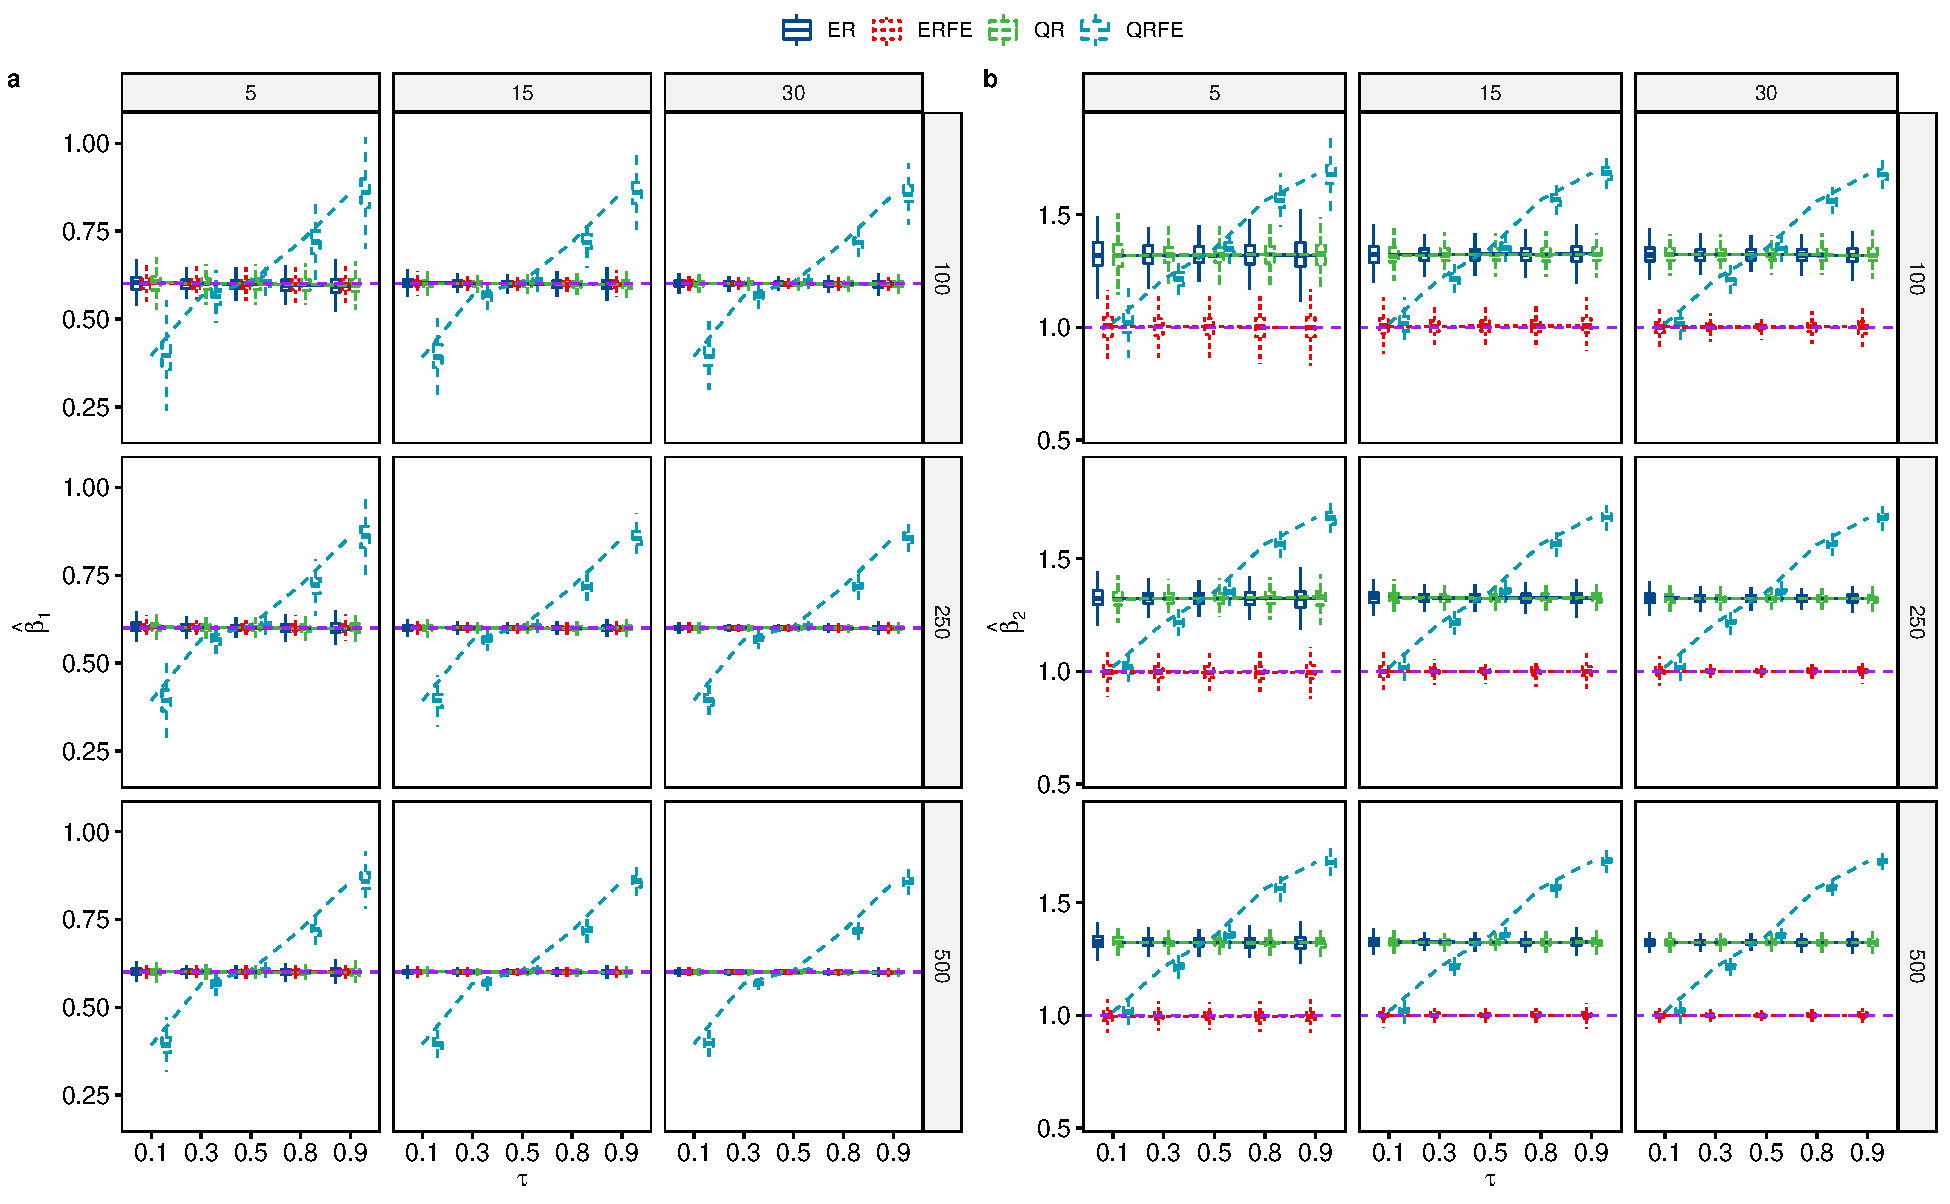
\includegraphics[width=0.8\linewidth]{Graph_supp/gstud1_erfe}
 \caption{Distribution of the coefficient estimates of the parameter $\beta_1$ (Figure \ref{fig:gstud1_erfe}\textbf{a}) and the parameter $\beta_2$ (Figure \ref{fig:gstud1_erfe}\textbf{b}) represented as boxplot according to the sample size $n\in(100,  \ 250,  \ 500),$ the repeated measurements $m=(5,\ 15,\ 30),$ the asymmetric points $\tau\in (0.1,  \ 0.3,  \  0.5, \  0.8,\ 0.9)$ and the error term $\varepsilon\sim\mathcal{T}(3)$ in the location-shift scenario.}\label{fig:gstud1_erfe}
\end{figure}
\end{center}

\begin{center}
\begin{figure}[H]
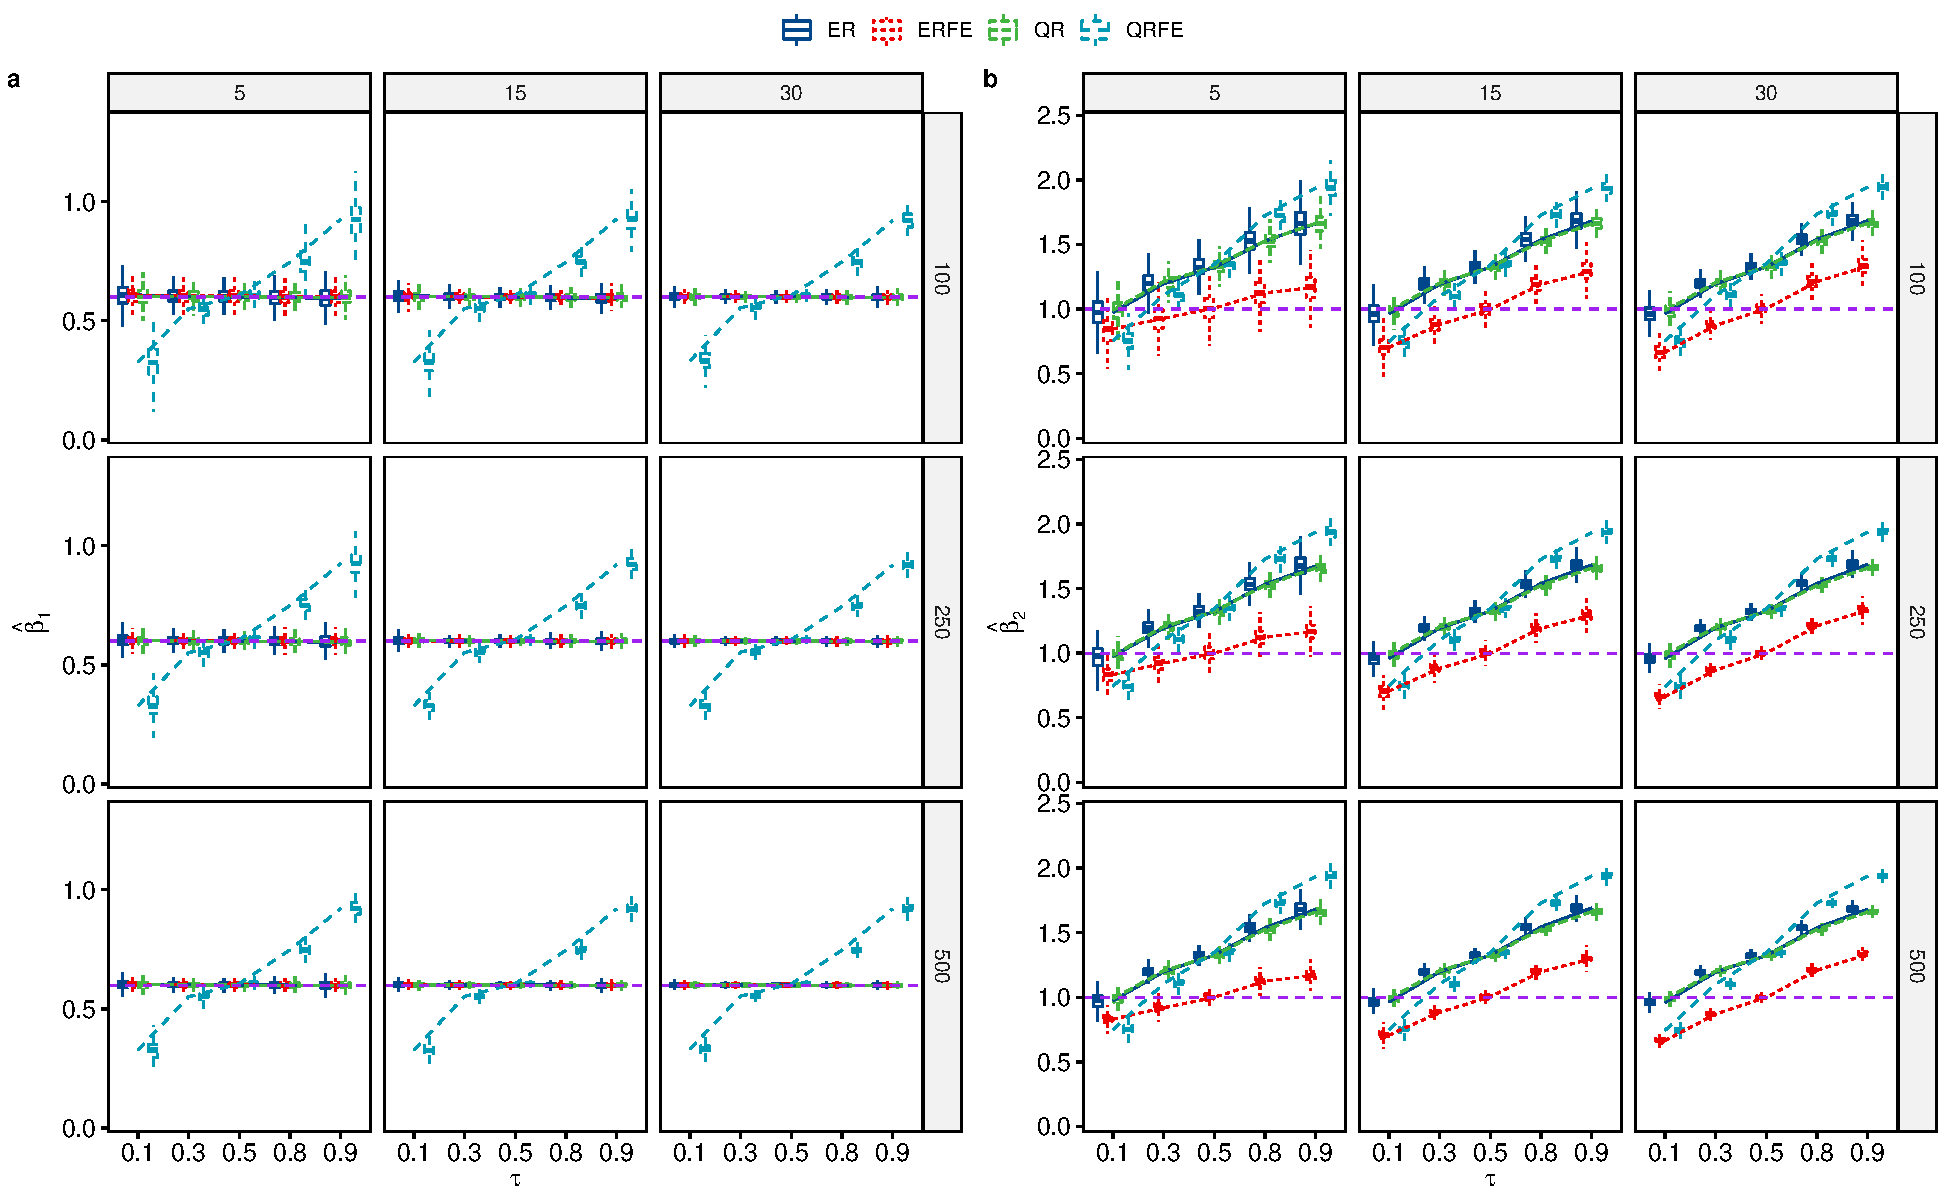
\includegraphics[width=0.8\linewidth]{Graph_supp/gstud2_erfe}
 \caption{Distribution of the coefficient estimates of the parameter $\beta_1$ (Figure \ref{fig:gstud2_erfe}\textbf{a}) and the parameter $\beta_2$ (Figure \ref{fig:gstud2_erfe}\textbf{b}) represented as boxplot according to the sample size $n\in(100,  \ 250,  \ 500),$ the repeated measurements $m=(5,\ 15,\ 30),$ the asymmetric points $\tau\in (0.1,  \ 0.3,  \  0.5, \  0.8,\ 0.9)$ and the error term $\varepsilon\sim\mathcal{T}(3)$ in the location-scale-shift scenario.}\label{fig:gstud2_erfe}
\end{figure}
\end{center} 

\begin{center}
\begin{figure}[H]
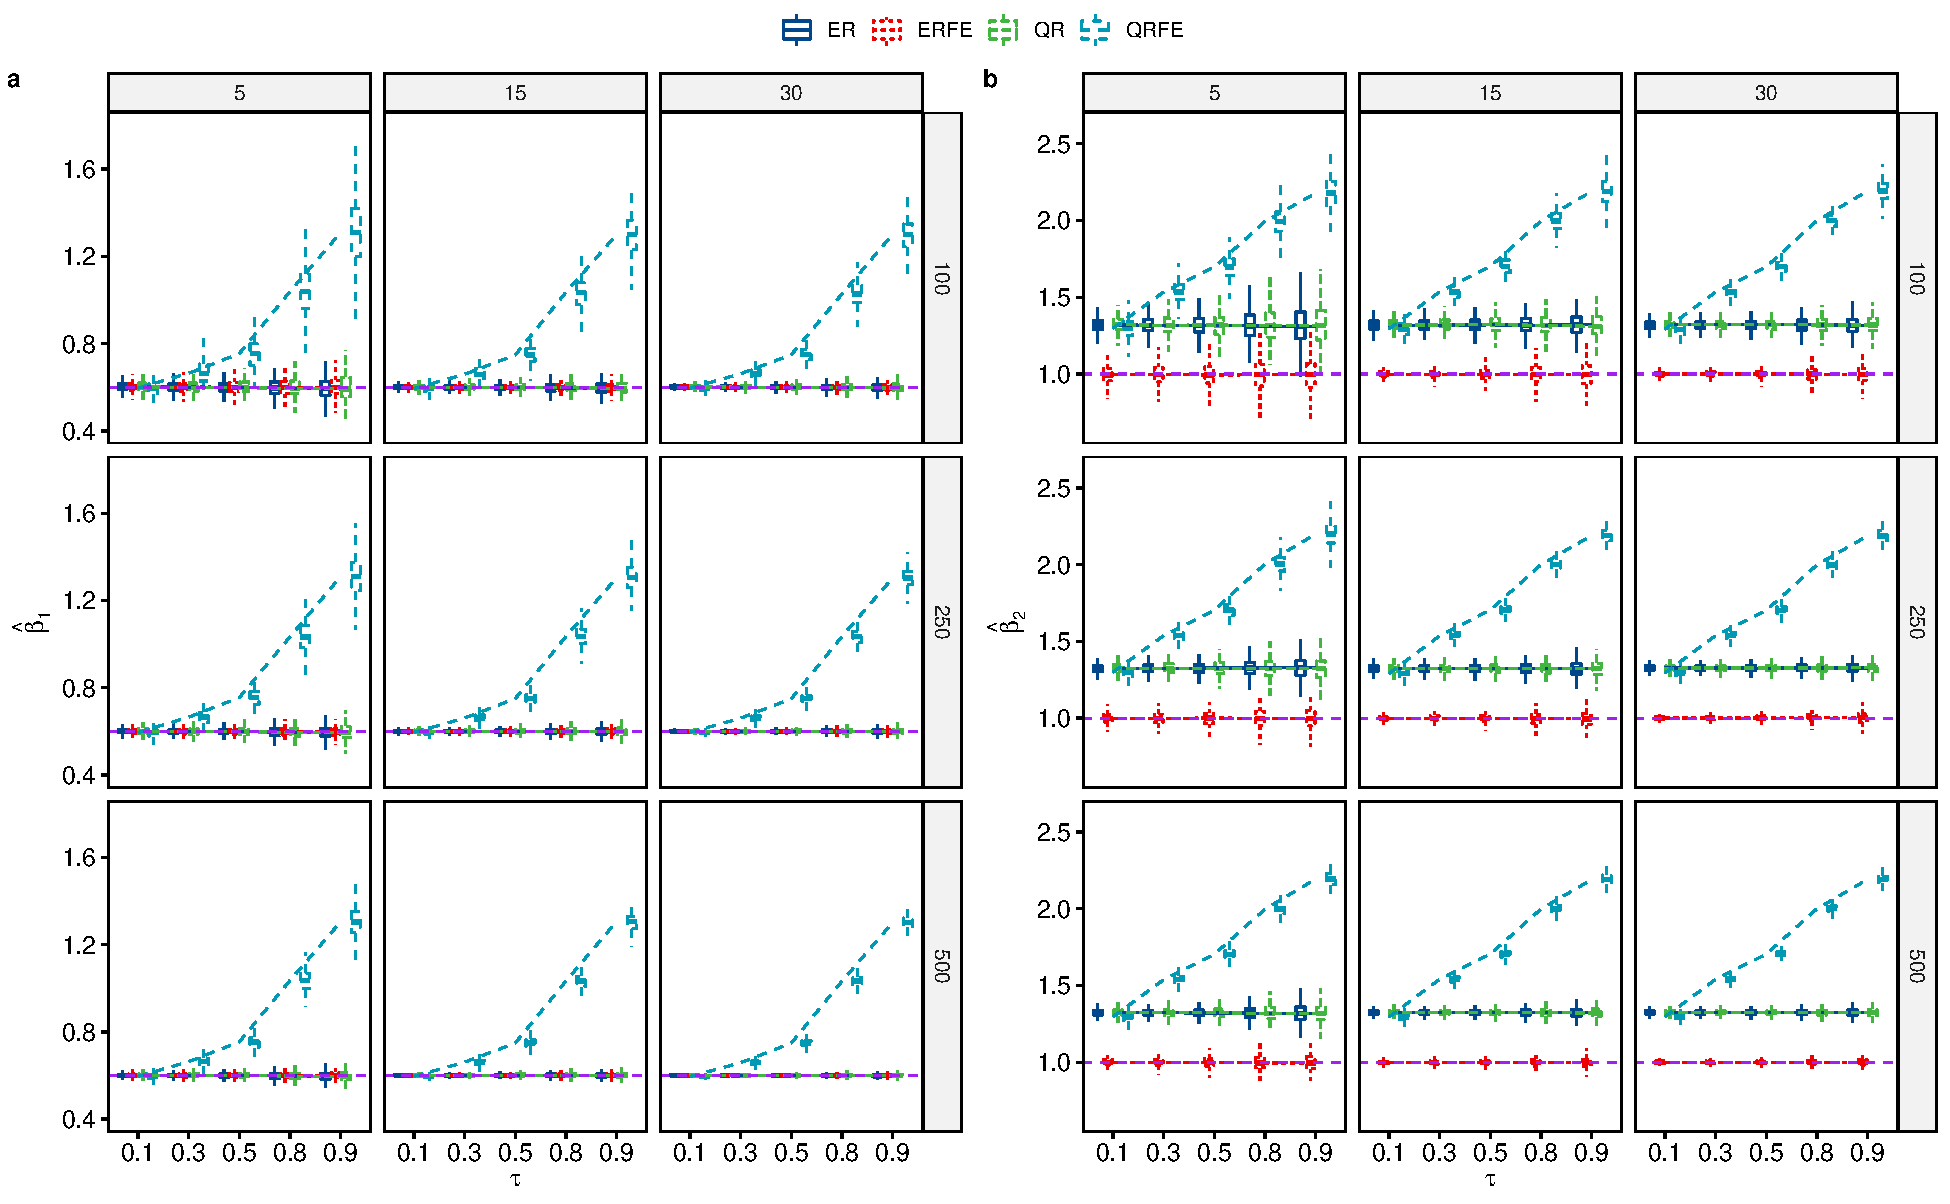
\includegraphics[width=0.8\linewidth]{Graph_supp/gchi1_erfe}
 \caption{Distribution of the coefficient estimates of the parameter $\beta_1$ (Figure \ref{fig:gchi1_erfe}\textbf{a}) and the parameter $\beta_2$ (Figure \ref{fig:gchi1_erfe}\textbf{b}) represented as boxplot according to the sample size $n\in(100,  \ 250,  \ 500),$ the repeated measurements $m=(5,\ 15,\ 30),$ the asymmetric points $\tau\in (0.1,  \ 0.3,  \  0.5, \  0.8,\ 0.9)$ and the error term $\varepsilon\sim\chi_2(3)$ in the location-shift scenario.}\label{fig:gchi1_erfe}
\end{figure}
\end{center}

\begin{center}
\begin{figure}[H]
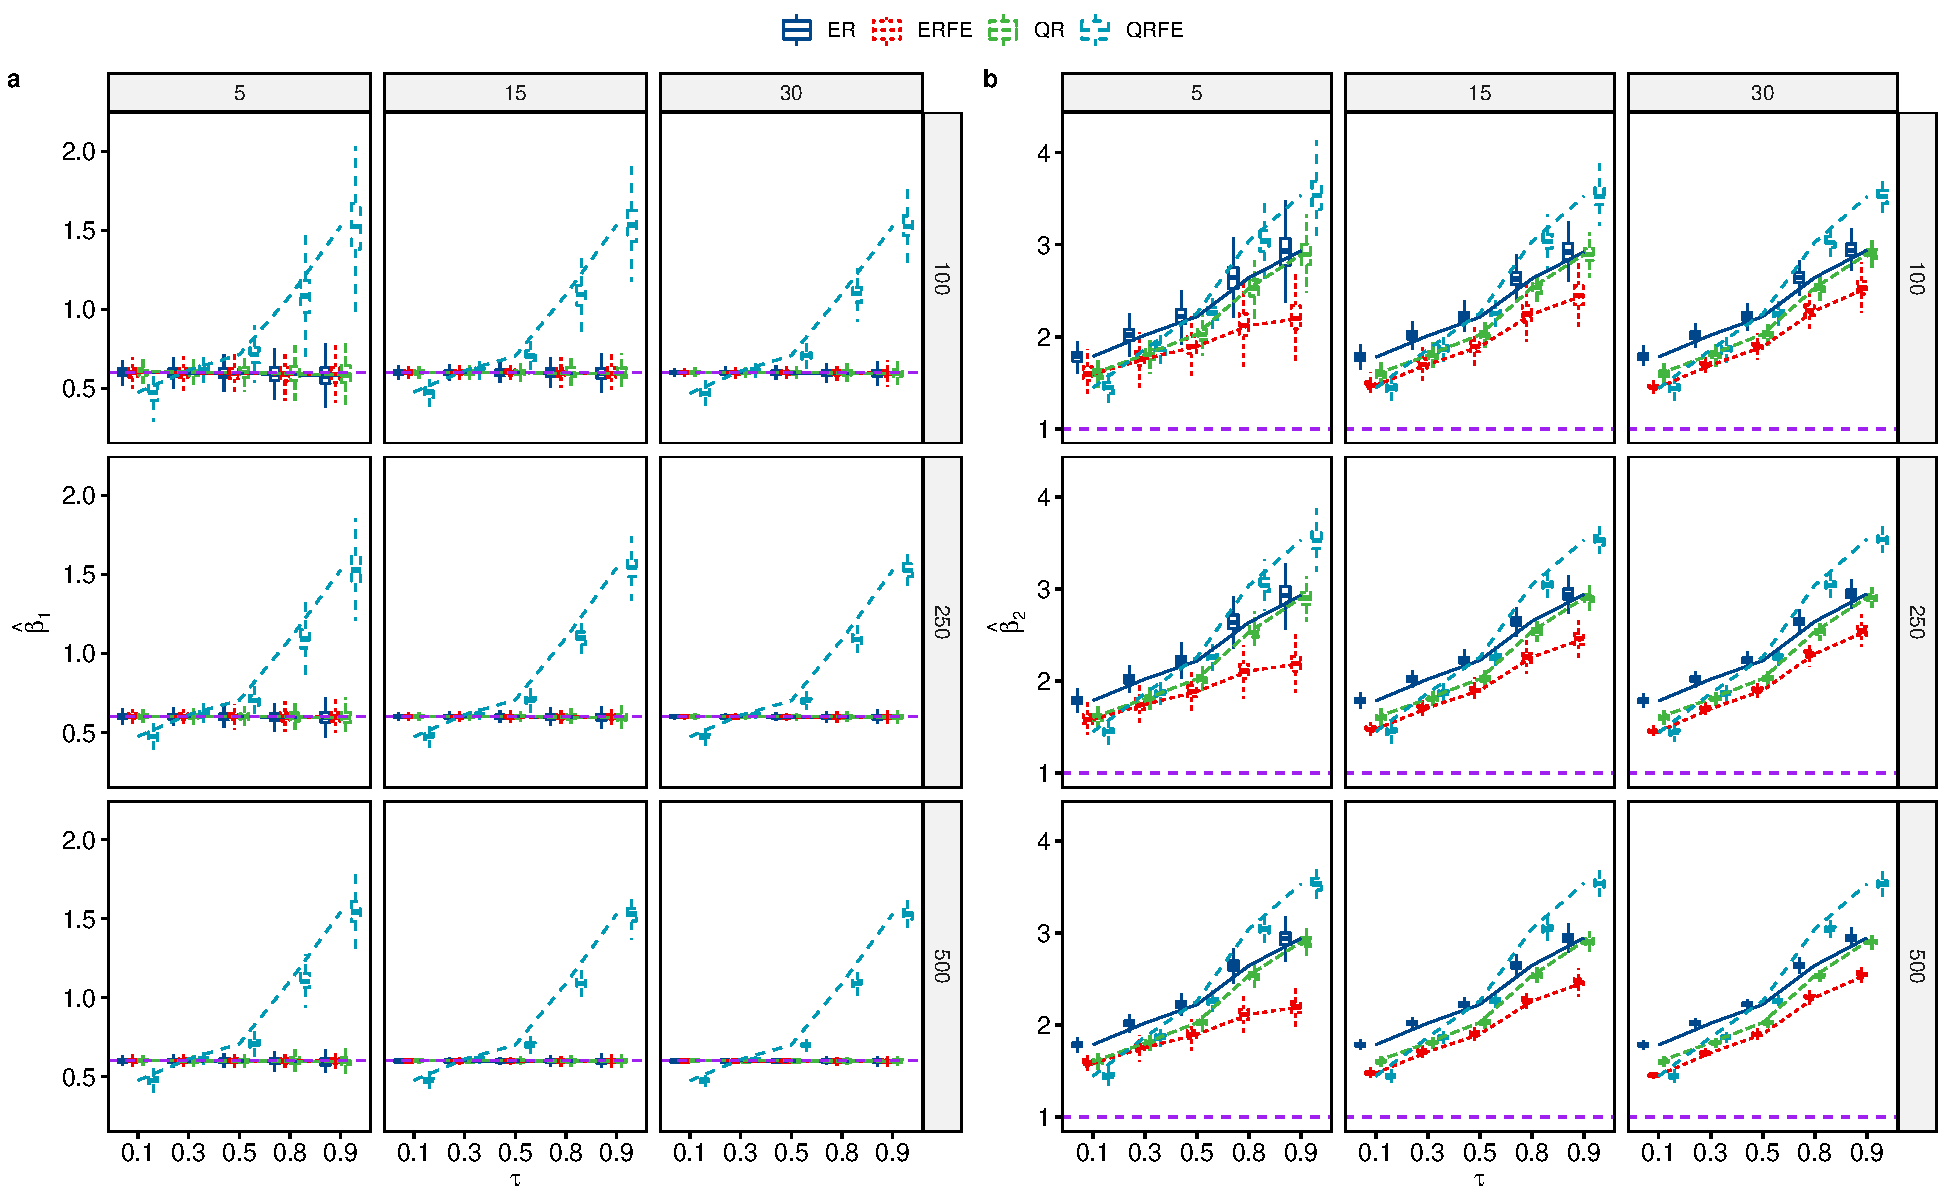
\includegraphics[width=0.8\linewidth]{Graph_supp/gchi2_erfe}
 \caption{Distribution of the coefficient estimates of the parameter $\beta_1$ (Figure \ref{fig:gchi2_erfe}\textbf{a}) and the parameter $\beta_2$ (Figure \ref{fig:gchi2_erfe}\textbf{b}) represented as boxplot according to the sample size $n\in(100,  \ 250,  \ 500),$ the repeated measurements $m=(5,\ 15,\ 30),$ the asymmetric points $\tau\in (0.1,  \ 0.3,  \  0.5, \  0.8,\ 0.9)$ and the error term $\varepsilon\sim\chi_2(3)$ in the location-scale-shift scenario.}\label{fig:gchi2_erfe}
\end{figure}
\end{center} 

\begin{center}
\begin{figure}[hbt!]
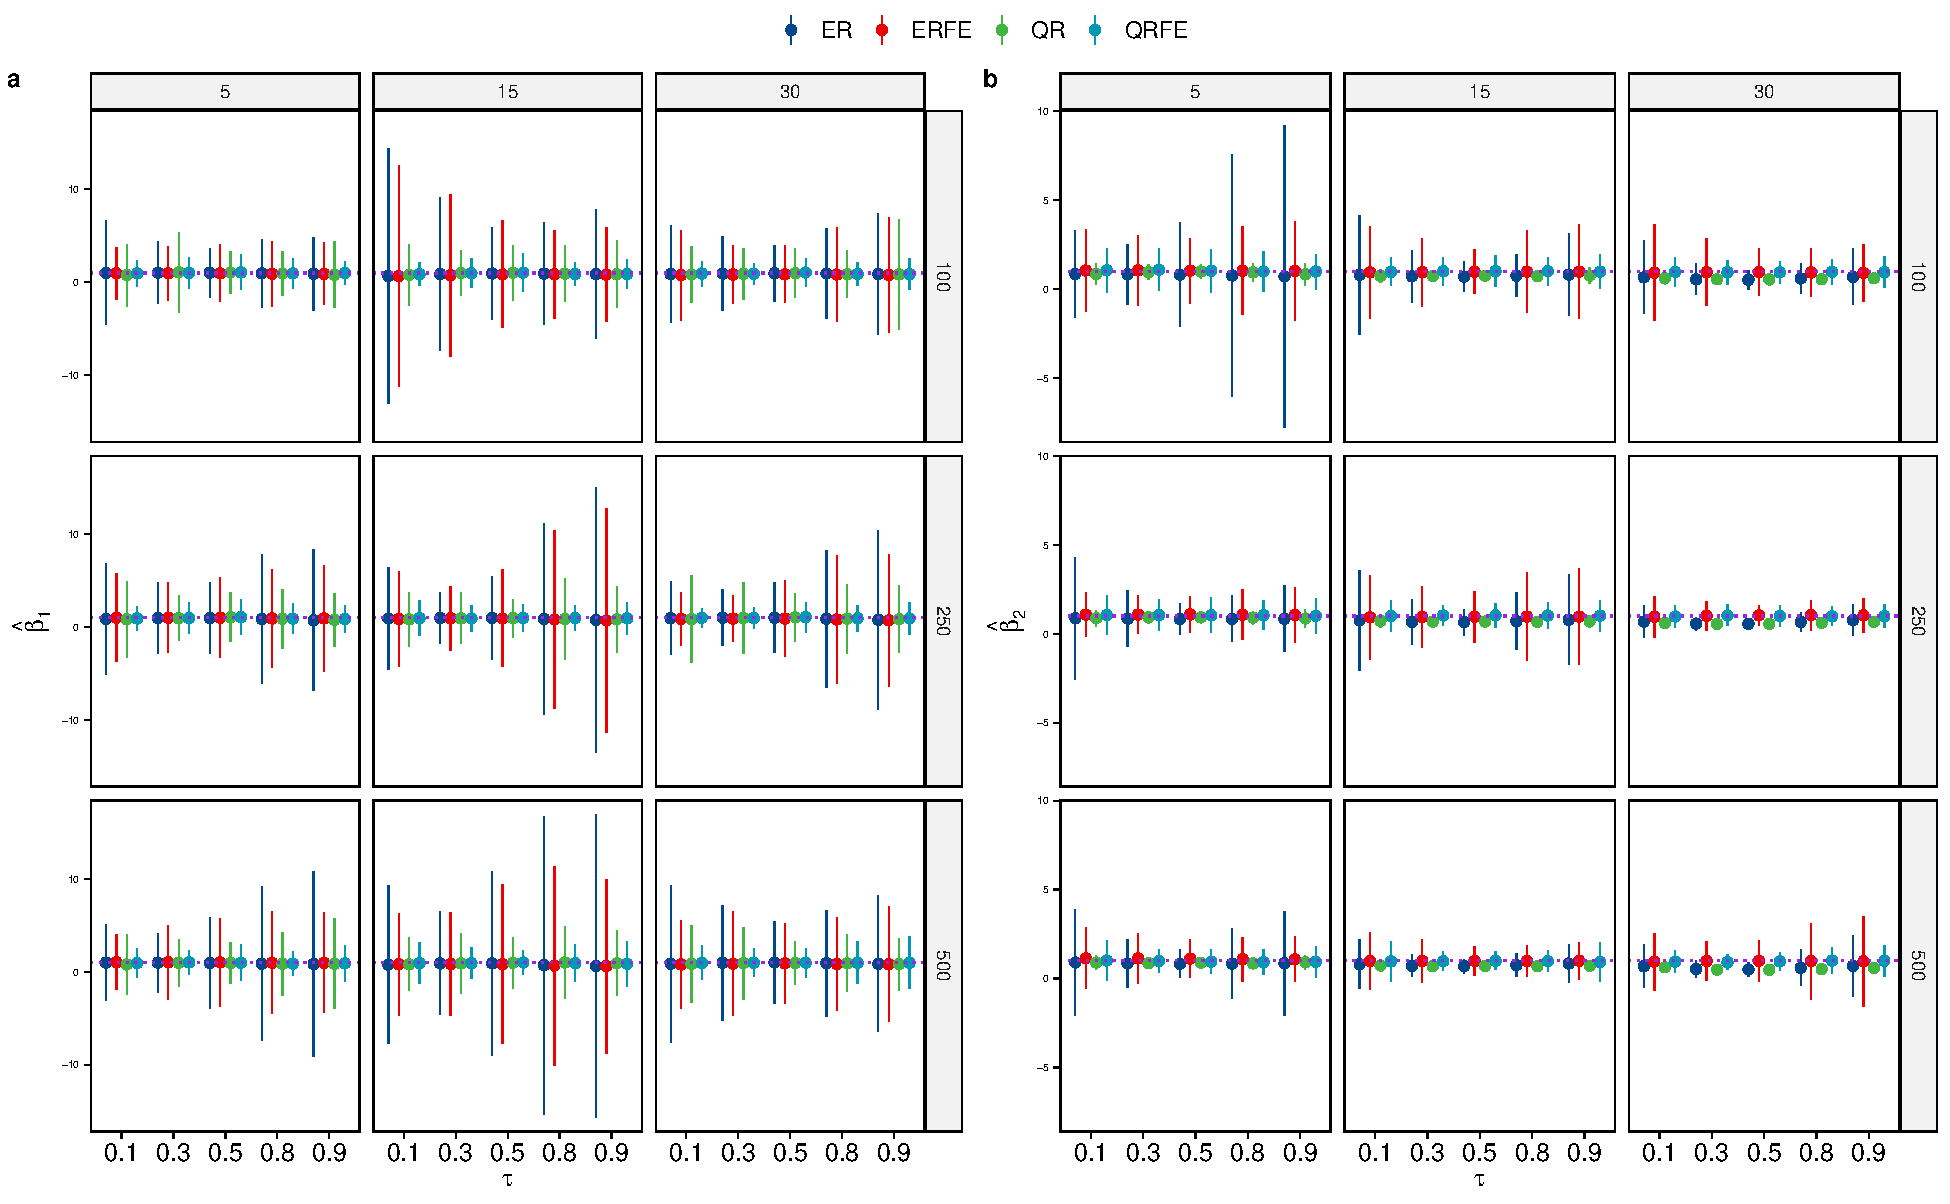
\includegraphics[width=0.75\linewidth]{Graph_supp/SdSe_stud_homo}
    \caption{Distribution of the ratio $\frac{\SE}{\SD}$ for the parameter estimate $\widehat{\beta}_1$ (Figure \ref{fig:SdSe_stud_homo}\textbf{a}) and the parameter estimate $\widehat{\beta}_2$ (Figure \ref{fig:SdSe_stud_homo}\textbf{b}) represented as an error plot with respect to the sample size $n\in(100,  \ 250,  \ 500),$ the repeated measurements $m=(5,\ 15,\ 30),$ the asymmetric points $\tau\in (0.1,  \ 0.3,  \  0.5, \  0.8,\ 0.9)$ and the error term $\varepsilon\sim\mathcal{T}(3)$ in the location-shift scenario.} \label{fig:SdSe_stud_homo}
\end{figure}
\end{center}

\begin{center}
\begin{figure}[hbt!]
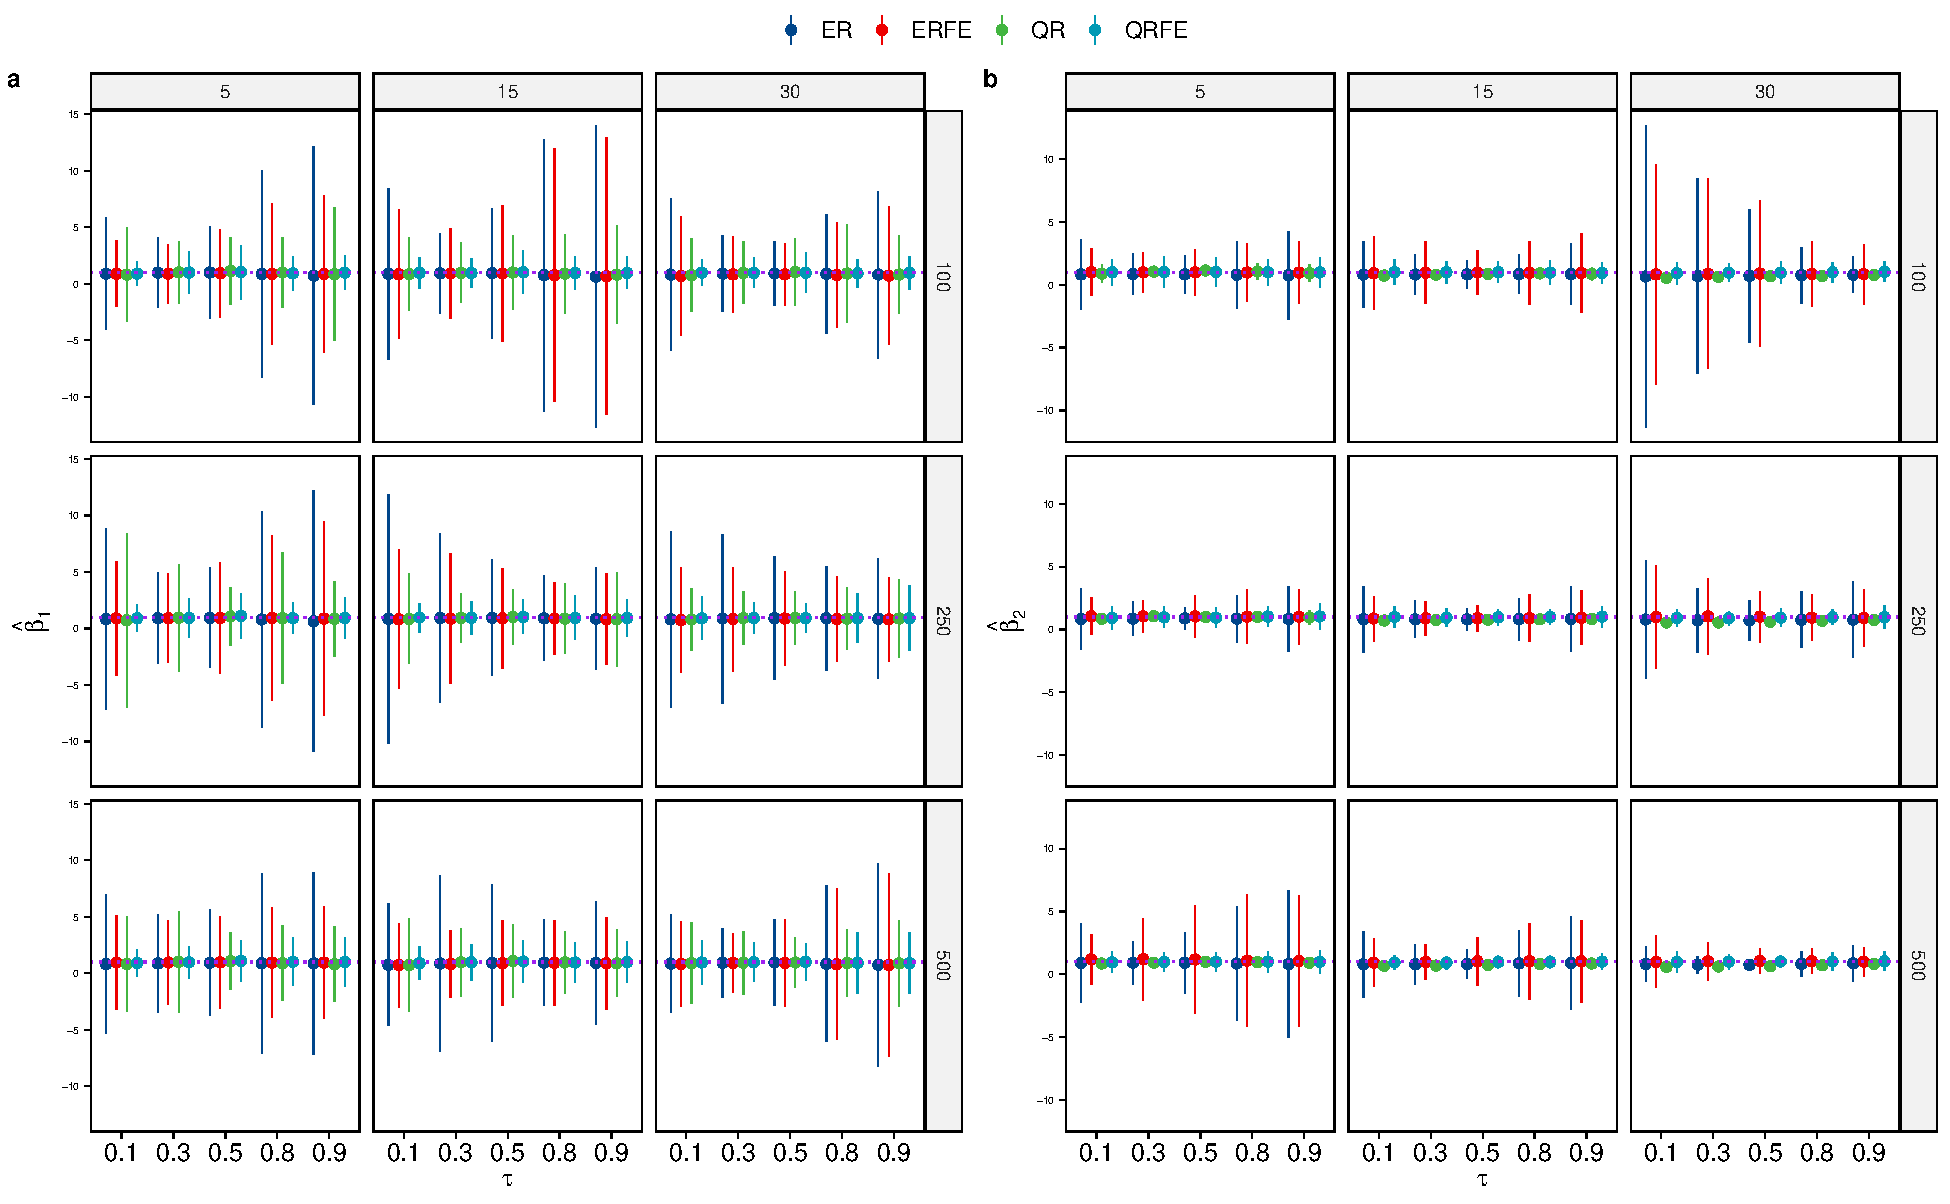
\includegraphics[width=0.75\linewidth]{Graph_supp/SdSe_stud_hetero}
    \caption{Distribution of the ratio $\frac{\SE}{\SD}$ for the parameter estimate $\widehat{\beta}_1$ (Figure \ref{fig:SdSe_stud_hetero}\textbf{a}) and the parameter estimate $\widehat{\beta}_2$ (Figure \ref{fig:SdSe_stud_hetero}\textbf{b}) represented as an error plot with respect to the sample size $n\in(100,  \ 250,  \ 500),$ the repeated measurements $m=(5,\ 15,\ 30),$ the asymmetric points $\tau\in (0.1,  \ 0.3,  \  0.5, \  0.8,\ 0.9)$ and the error term $\varepsilon\sim\mathcal{T}(3)$ in the location-scale-shift scenario.} \label{fig:SdSe_stud_hetero}
\end{figure}
\end{center}

\begin{center}
\begin{figure}[hbt!]
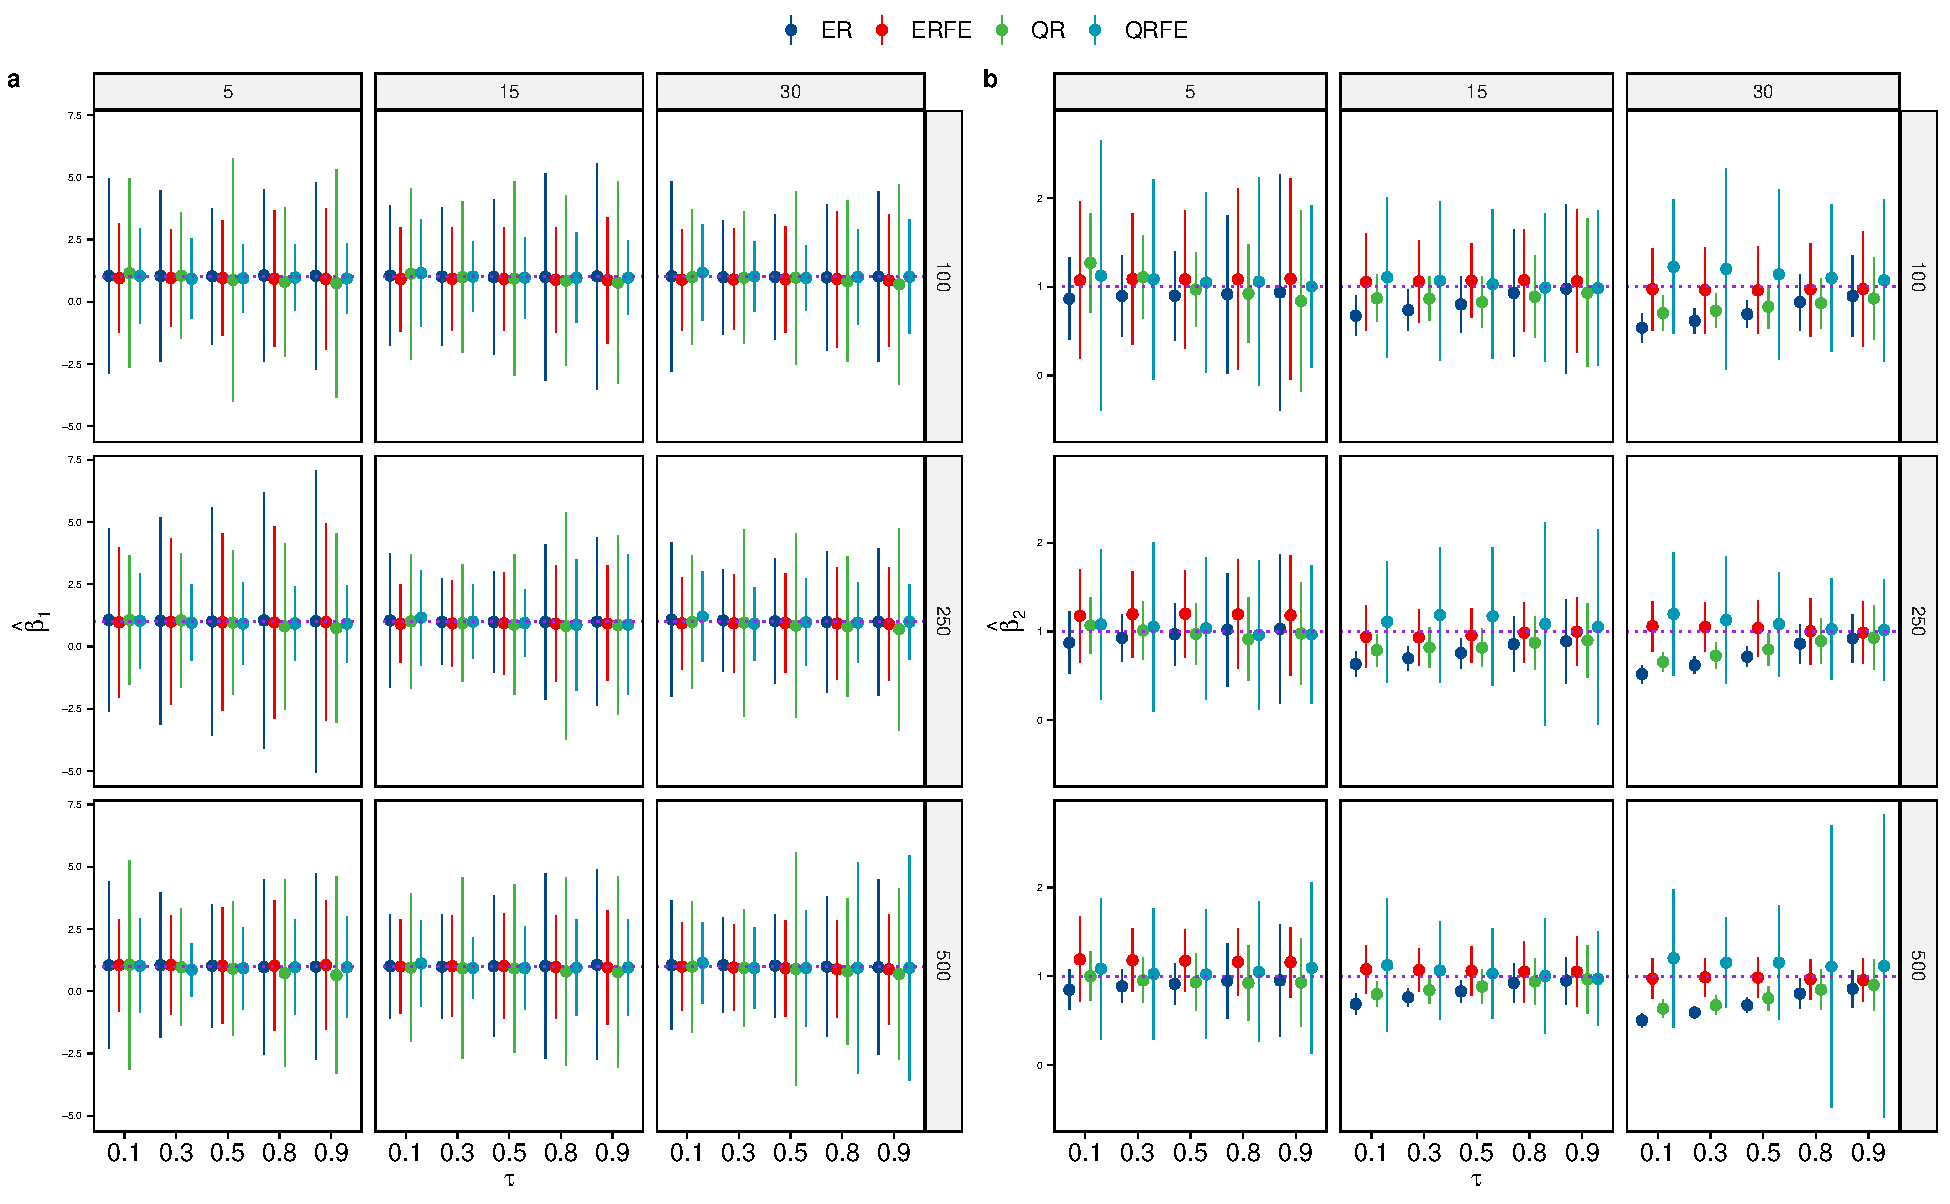
\includegraphics[width=0.75\linewidth]{Graph_supp/SdSe_chi2_homo}
    \caption{Distribution of the ratio $\frac{\SE}{\SD}$ for the parameter estimate $\widehat{\beta}_1$ (Figure \ref{fig:SdSe_chi2_homo}\textbf{a}) and the parameter estimate $\widehat{\beta}_2$ (Figure \ref{fig:SdSe_chi2_homo}\textbf{b}) represented as an error plot with respect to the sample size $n\in(100,  \ 250,  \ 500),$ the repeated measurements $m=(5,\ 15,\ 30),$ the asymmetric points $\tau\in (0.1,  \ 0.3,  \  0.5, \  0.8,\ 0.9)$ and the error term $\varepsilon\sim\chi_2(3)$ in the location-shift scenario.} \label{fig:SdSe_chi2_homo}
\end{figure}
\end{center}

\begin{center}
\begin{figure}[hbt!]
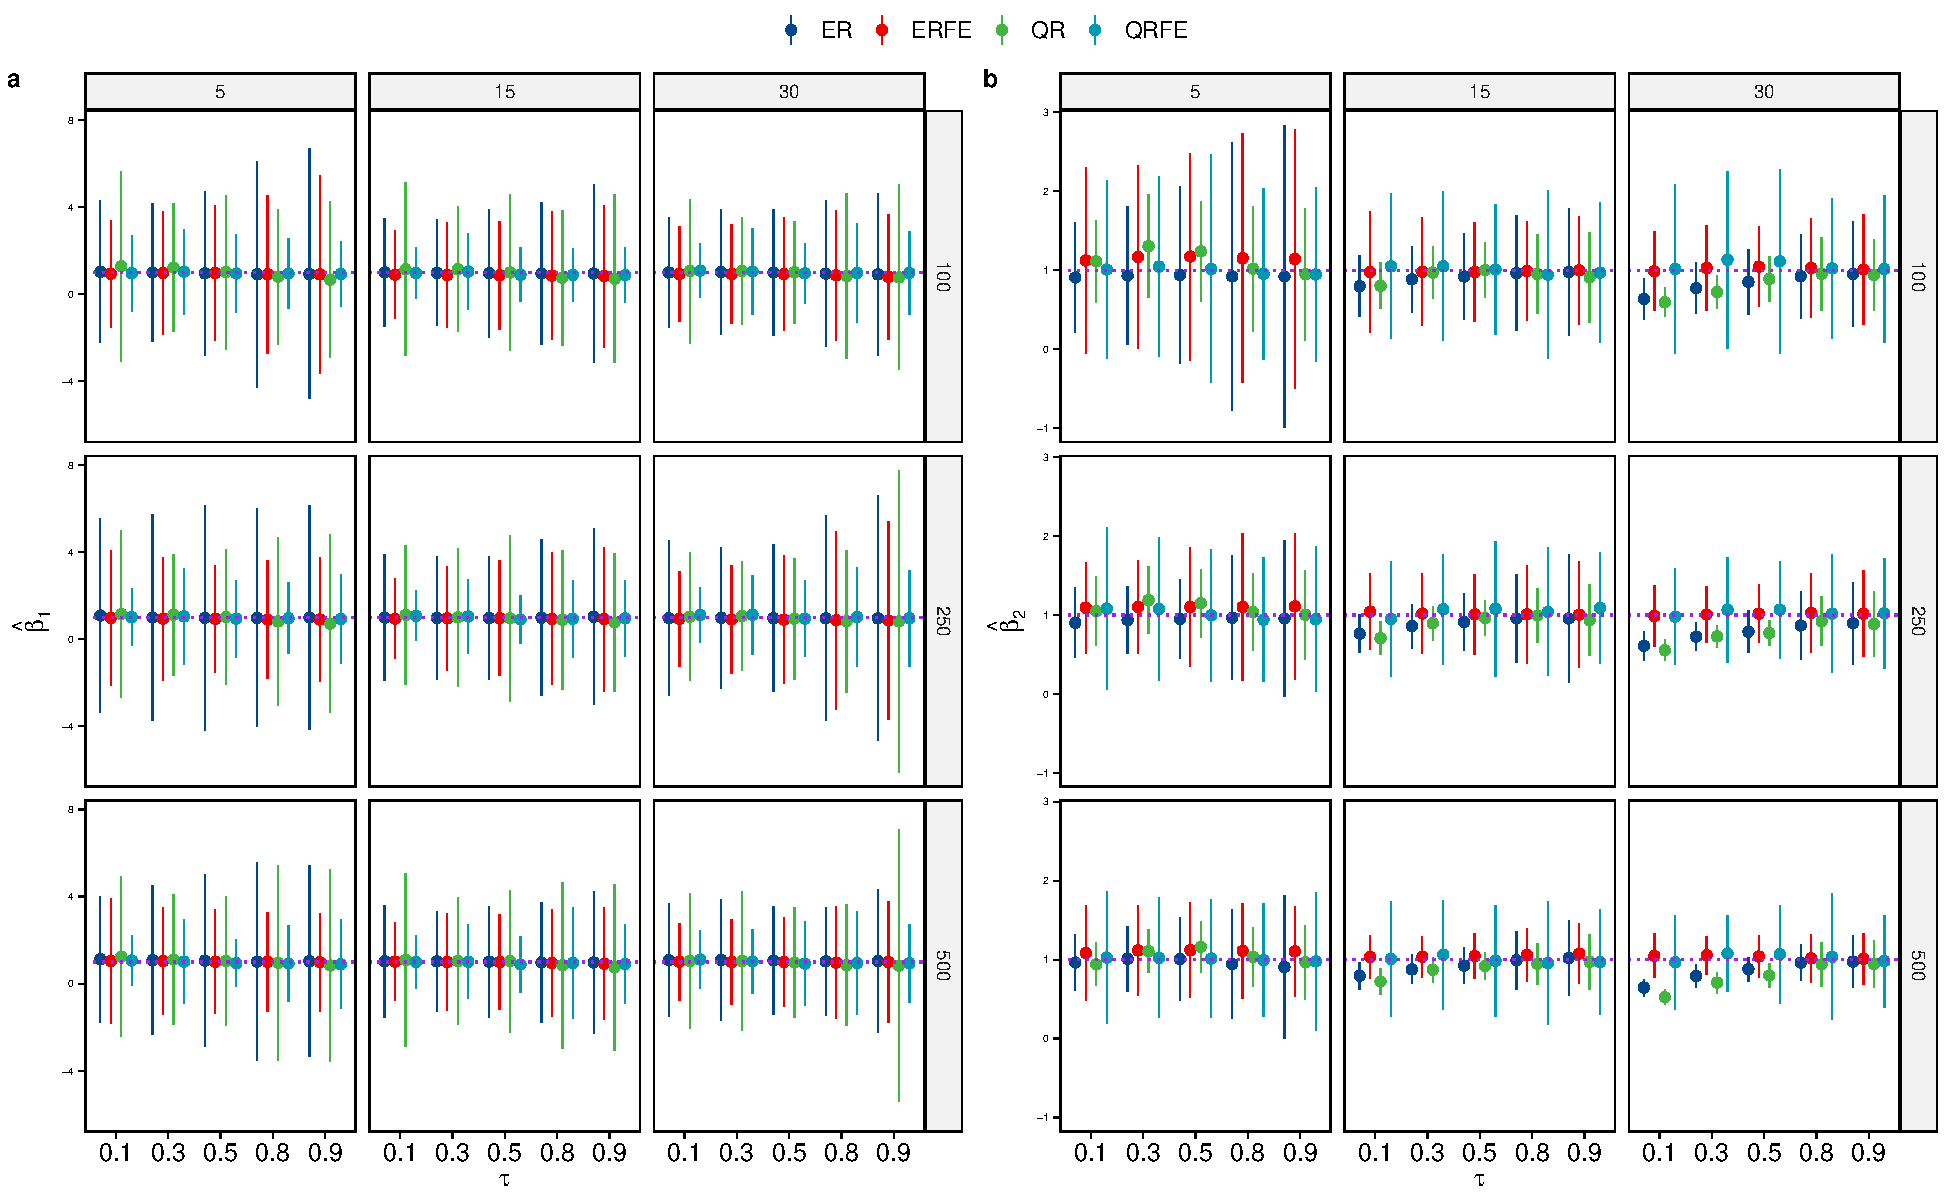
\includegraphics[width=0.75\linewidth]{Graph_supp/SdSe_chi2_hetero}
    \caption{Distribution of the ratio $\frac{\SE}{\SD}$ for the parameter estimate $\widehat{\beta}_1$ (Figure \ref{fig:SdSe_chi2_hetero}\textbf{a}) and the parameter estimate $\widehat{\beta}_2$ (Figure \ref{fig:SdSe_chi2_hetero}\textbf{b}) represented as an error plot with respect to the sample size $n\in(100,  \ 250,  \ 500),$ the repeated measurements $m=(5,\ 15,\ 30),$ the asymmetric points $\tau\in (0.1,  \ 0.3,  \  0.5, \  0.8,\ 0.9)$ and the error term $\varepsilon\sim\chi_2(3)$ in the location-scale-shift scenario.} \label{fig:SdSe_chi2_hetero}
\end{figure}
\end{center}

\clearpage
\bibliographystyle{apalike}
\bibliography{bib_fix_effect.bib}
\end{document}
